\documentclass[12pt,a4paper,twoside,openright]{book}
\pagestyle{headings} % page style (for heading etc)

\usepackage[a4paper]{meta-donnees} % University template
\usepackage[utf8]{inputenc} % UTF-8 for accents
\usepackage[T1]{fontenc} % UTF-8 for accents
\usepackage[english,french]{babel} % for langages
\usepackage{lipsum}
%\usepackage{epigraph} % for quotations at the beginning of each chapter
%\setlength{\epigraphwidth}{15cm}

% amsmath and amssymb packages, useful for mathematical formulas and symbols
\usepackage{amsmath,amssymb,amsfonts,mathrsfs}

\usepackage{graphicx} % no idea but was needed in the suppinfo of chapter 2

% cite package, to clean up citations in the main text.
\usepackage{cite}

% Use nameref to cite supporting information files (see Supporting Information section for more info)
\usepackage{nameref,hyperref}

% BiBTeX style
\bibliographystyle{unsrt}

% Remove brackets from numbering in List of References
\makeatletter
\renewcommand{\@biblabel}[1]{\quad#1.}
\makeatother


%%%%%%%%%%% Custom environment %%%%%%%%%%%
\newenvironment{acknowledgements}{
\newpage
\null \vspace{\stretch{1}}
\begin{center}\bfseries Acknowledgements \end{center}
}
{\vfill \null}

\newenvironment{abstract}{
\clearpage
\begin{center}\bfseries \abstractname \end{center}
}
{\vfill \null}
%%%%%%%%%%%%%%%%%%%%%%%%%%%%%%%%%%%%%%%%%%%

%%%%%%%%%%%%% Custom commands %%%%%%%%%%%%%

%%%%%%%%%%%%%%%%%%%%%%%%%%%%%%%%%%%%%%%%%%%

\begin{document}

% les lignes en bas sont à insérer obligatoirement après \begin{document}

%%%%%%%%%%%%%%%%%%%%%%%%%%%%%%%%%%%%%%%%%%%%%%%%%%%%%%
%%             Commandes Meta-données               %%
%%   à renseigner par les auteurs pour générer      %%
%%     la couverture modèle Univ. Grenoble          %%
%%%%%%%%%%%%%%%%%%%%%%%%%%%%%%%%%%%%%%%%%%%%%%%%%%%%%%

%\Sethpageshift{???mm}   %%optionnel : à décommenter si besoin pour ajout d'espace afin de center la couvérture horizontalement (valeur par défaut est -5.5mm)
%\Setvpageshift{???mm}   %%optionnel : à décommenter si besoin pour ajout d'espace afin de center la couvérture verticalement (valeur par défaut est -15.5mm)

%\Universite{}    %%optionnel : à décommenter et à renseigenr si vous voulez changer le non d'université
%\Grade{}         %%optionnel : à décommenter et à renseigenr si vous voulez changer le grade
\Specialite{Biologie cellulaire}
\Arrete{25 mai 2016} % ATTENTION, A VERIFIER CHAQUE ANNEE
\Auteur{Nils GIORDANO}
\Directeur{Johannes GEISELMANN}
\CoDirecteur{Hidde DE JONG}
\Laboratoire{Laboratoire Interdisciplinaire de Physique}
\EcoleDoctorale{Chimie et Sciences du Vivant}  
\Titre{Microbial growth control in changing environments}
\Soustitre{Theoretical and experimental study of resource allocation in \textit{Escherichia coli}}      %%optionnel : à décommenter et à renseigenr si présence d'un sous-titre de thèse
\Depot{23 mars 2017} %% DATE DE LA SOUTENANCE

% Commande pour création de nouvelles catégories dans le jury:
%\UGTNewJuryCategory{...NomDeLaCategorie...}{...Definition...}
% Exemple \UGTNewJuryCategory{UGTFamille}{Membre de la famille} que nous ajoutons dans la commande \Jury ci-dessous sous la forme \UGTFamille{Jean Rousseau}{(...titre_et_affiliation...s'il_y_en_a...)}

\Jury{
%\UGTPresident{M, Olivier BERNARD}{Chargé de recherche, Inria, Nice -- Sophia-Antipolis (à confirmer pour président)}     %% 2ème examinateur
%\UGTPresidente{...Civilité, Prénom-et-Nom...}{...titre-et-affiliation...}
\UGTPresidente{Mme, Irina MIHALCESCU}{Prof.}{Univ. Grenoble Alpes}

\UGTRapporteur{M, Matthew SCOTT}{Assoc. Prof.}{Univ. of Waterloo (CA)}      %% 1er rapporteur
\UGTRapporteur{M, Guy-Bart STAN}{Reader}{Imp. College London (UK)}      %% second rapporteur

\UGTExaminateur{M, Olivier BERNARD}{DR}{Inria Sophia-Antipolis}     %% 2ème examinateur
\UGTExaminateur{M, Jean-Luc GOUZÉ}{DR}{Inria Sophia-Antipolis}
\UGTExaminateur{M, Matthieu JULES}{CR}{Inra Grignon}     %% 1er examinateur


%\noindent\hfil\rule{4cm}{0.1pt}\hfil
%
%\vspace{0.3cm}

%\UGTDirecteur{M, Johannes GEISELMANN}{Prof.}{Univ. Grenoble Alpes}       %% Directeur de thèse
%\UGTCoDirecteur{M, Hidde DE JONG}{DR}{Inria Grenoble}     %% Co-Directeur de thèse s'il y en a
%\UGTInvitee{...Civilité, Prénom-et-Nom...}{...titre-et-affiliation...}
}

\MakeUGthesePDG    %% très important pour générer la couvérture de thèse


\cleardoublepage
\null \vspace{\stretch{1}}
\begin{flushright}
\textit{A Kiki mon Raton Laveur...}
\end{flushright}
\vspace{\stretch{2}}\null

\cleardoublepage
\begin{acknowledgements}
Special thanks to Alan Turing, without whom this PDF file would not have existed, leading to the destruction of more trees.
\end{acknowledgements}

\selectlanguage{english}
\begin{abstract}
\lipsum[2]
\end{abstract}

\selectlanguage{french}
\begin{abstract}
\lipsum[2]
\end{abstract}
\selectlanguage{english}


\tableofcontents

%%%%%%%%%%%%%%%%%%%%%%%%%%%%%%%%%%%%%%%%%%%%%%%%%%%%%%%%%%%%%%%%%%%%%%%%%%%%%%%%%%%%%%%%%%%%%%%%

\chapter{Introduction}
\label{chap:introduction}

\textit{"There's an infinity of things that have never been done before, and most of those things are not worth doing."} -- Jeremy Fox, \textit{Dynamic Ecology}~\cite{fox_how_2016}

\begin{center}
\noindent\rule{4cm}{0.1pt}
\end{center}

\selectlanguage{french}
\begin{chapter_summary}{Introduction}
Malgré leur apparente simplicité, les microorganismes sont des êtres vivants complexes capables de survivre dans les milieux les plus extrêmes.
Une telle ubiquité repose en partie sur leurs excellentes capacités d'adaptation.
En effet, \textit{via} l'information stockée dans son ADN, une cellule microbienne est capable, par la production des protéines nécessaires, d'assimiler et de se répliquer à partir d'une grande variété de nutriments.
Ce mécanisme, que l'on appelle l'expression génétique, permet donc à la cellule de réguler sa composition en fonction des conditions environnementales.
Chaque composant cellulaire est initialement issu des ressources trouvées dans l'environnement.
Par l'expression génétique, la machinerie cellulaire résout donc un problème de distribution des ressources: un bien commun (les nutriments) est partagé entre plusieurs milliers de bénéficiaires potentiels (les protéines et autres macromolécules).

Selon quels critères les ressources sont-elles distribuées dans la cellule ?
Le comportement de la plupart des systèmes vivants peut s'expliquer par les principes de la sélection naturelle.
En définissant des facteurs de \textit{fitness} (adaptation au milieu), on peut généralement identifier des objectifs permettant à l'organisme de maximiser sa descendance, et donc de persister sur le long terme dans un milieu donné.
Ces facteurs et surtout leurs importances relatives, peuvent s'avérer extrêmement complexes à identifier, 
ce qui est notamment le cas chez les microorganismes.
Cependant, de nombreuses études ont pu montrer que la maximisation du taux de croissance (ou taux de réplication) est un facteur qui semble commun à de nombreux microorganismes, et qui permet d'expliquer à lui seul une grande variété de comportements.

Peut-on, à l'aide d'un tel principe universel, formaliser la croissance des microorganismes en lois simples, analogues à celle que l'on peut trouver dans d'autres domaines des sciences comme la physique ?
Historiquement, la première tentative d'établissement de lois fondamentales de la physiologie microbienne  fut la découverte de la loi de Monod il y a plus de 60 ans (Fig.~\ref{fig:monod_law} et Eq.~\ref{eq:monod_law}).
Elle montre que le taux de croissance d'un microorganisme suit une loi hyperbolique de la concentration du nutriment limitant dans le milieu.
Depuis, d'autres lois fondamentales ont pu être identifiées.
L'une d'entre elles est une loi de croissance qui décrit la relation linéaire existante entre la concentration en ribosomes dans la cellule et le taux de croissance de l'organisme (Fig.~\ref{fig:scott_rnaprot}).
De manière étonnante, quels que soient les détails moléculaires qui permettent cette adaptation, cette loi émerge lorsque la cellule cherche à maximiser son taux de croissance dans chaque environnement.

Bien que répandues chez de nombreux microorganismes, ces lois se limitent à un état bien particulier qu'on appelle croissance à l'état stationnaire.
Cet état est atteint lorsque l'organisme se multiplie pendant suffisamment longtemps dans un environnement stable (Fig.~\ref{fig:growth_curve}).
Il s'avère très pratique pour les études théoriques et expérimentales, notamment car les composants de la cellule ne changent plus au cours du temps, ce qui lui vaut aussi l'appellation de croissance équilibrée (\textit{balanced growth}).
Mais cet état a beau être pratique, il est très loin des conditions rencontrées par les microorganismes dans leur milieu de vie naturel.
Ces derniers sont en effet plutôt soumis à des environnements changeants, où les éléments chimiques indispensables à la croissance sont rares, et sont donc les objets d'une rude compétition.
Pour quelles raisons les microorganismes seraient-ils optimisés pour un état de croissance qu'ils n'ont quasiment jamais rencontré au cours de leur évolution ?
Si comme on s'y attend ces systèmes sont plutôt adaptés à des environnements variables, ratons-nous quelque chose en ne les étudiant qu'en conditions stables ?

Dans cette thèse, nous nous proposons ainsi d'étendre les études des lois de croissance en adoptant une perspective dynamique, c'est-à-dire, en environnements variables : quelles stratégies dynamiques les microorganismes suivent-ils pour redistribuer leurs ressources lors d'un changement environnemental ?
Cette question sera développée en deux grands axes d'étude.

Quelles sont les meilleures stratégies de distribution des ressources si, comme pour les lois de croissance à l'état stationnaire, la production de biomasse est le seul critère optimisé par la cellule ?
Répondre à cette question est une étape nécessaire pour évaluer dans quelles mesures les critères d'optimisation dynamique peuvent différer de ceux à l'état stationnaire, et donc, de tester si les pressions évolutives s'appliquent effectivement différemment entre environnements stables et dynamiques.
Cette preuve de concept reposera sur un modèle de la distribution des ressources dans une cellule microbienne, qui sera utilisé pour déterminer quelle est la manière dynamique optimale pour la cellule de distribuer ses ressources lors d'un changement d'environnement (Chapitre~\ref{chap:theory}).

Les prédictions faites seront ensuite testées expérimentalement.
Nous chercherons donc à mesurer la distribution des ressources chez \textit{Escherichia coli} lors d'une transition de croissance (Chapitre~\ref{chap:experiments}).
Nous montrerons comment l'utilisation de marqueurs fluorescents des ribosomes, d'un dispositif microfluidique de culture continue, et de méthodes originales d'analyse des séries temporelles, permet d'observer et de reconstruire l'allocation des ressources au cours d'une transition brutale du milieu, notamment la transition d'un milieu pauvre vers un milieu riche (\textit{nutrient upshift}).
\end{chapter_summary}
\selectlanguage{english}

\begin{center}
\noindent\rule{4cm}{0.1pt}
\end{center}

\section*{Beginning of Chapter \thechapter}
\section{Context}
\label{sec:context}

\subsection{Self-replication is a resource allocation problem}

At every moment of our lives, we are surrounded by billions of microscopic organisms.
They sustain themselves by harvesting energy from their environment in the form of organic matter, highly reactive chemicals, or light~\cite{madigan_biology_2006,schaechter_microbe_2006}.
While most of our cells are kept in a stable and friendly internal environment (temperature, oxygenation, nutrient abundance, ...), microorganisms have evolved to constantly adapt their physiology to strongly variable conditions~\cite{mcarthur_microbial_2006,menge_nitrogen_2012,hobbie_microbes_2013,
savageau_escherichia_1983,savageau_demand_1998,blount_unexhausted_2015,vanelsas_survival_2011}.
Not without success, because microbes have been found to survive almost everywhere, sometimes in the strangest places that were initially thought unsuitable for life~\cite{rothschild_life_2001,nicholson_transcriptomic_2012,madigan_biology_2006,schaechter_microbe_2006}.
Such ubiquity translates a strong potential for adaptation.
The model organism \textit{Escherichia coli}, a bacterium first isolated from our intestinal tract, is capable of growing on dozens of different carbon sources through changes in the expression of thousands of genes~\cite{zimmer_microcosm:_2009}.

Microorganisms, along with all living cells, are mainly constituted of polymers (DNA, RNA, proteins) consisting of many repeated subunits (nucleotides, amino acids).
The information about their sequences is stored in the form of genes, physically located on the DNA.
Gene expression is the process by which this information is used in the synthesis of a functional final product (protein or RNA).
The gene expression machinery (itself constituted of RNA and proteins) synthesizes gene products after binding to target sequences either by transcription (promoter on the DNA), or translation (ribosome binding site on the messaging RNA).
In a given cell, there are roughly as many different target sequences as genes~\cite{keseler_ecocyc_2013}, which ensures that not all products are synthesized at the same rate.
Furthermore, some of these products specifically bind some promoters and stimulate or repress promoter activity and hence gene expression.
These products are called transcription factors and allow, in addition to other mechanisms, the regulation of cell composition.

The reorganization of gene expression controls the abundance of enzymes and ribozymes that catalyze the biochemical reactions allowing the cell to perform different functions.
For instance, assimilating a given nutrient involves the synthesis of the corresponding uptake protein and of the metabolic enzymes converting the nutrients into reducing power, nucleotides and amino acids~\cite{schaechter_microbe_2006}.
These precursors are then used to produce new macromolecules, closing the loop of self-replication.
In order to optimize the overall process in different environmental conditions, the cell must adjust the abundance of every enzyme involved in this network of biochemical reactions.
By doing so, the cell actually solves a resource allocation problem, where a common wealth (precursors) has to be distributed over thousands of potential beneficiaries (proteins and other macromolecules).

\subsection{Optimizing biomass production yields a competitive advantage}

Which allocation of resources is optimal for a living cell?
Systems capable of Darwinian evolution sustain themselves in the long run by fitting to their environment~\cite{dawkins_selfish_1976}.
Living cells with the best fitness are more likely to survive, replicate, and through long-term competition, eliminate their siblings.
The optimization criteria that quantitatively measure fitness are called fitness factors.
Whether they apply at the species, the population, the organism, or even the gene level has long been debated~\cite{dawkins_selfish_1976}.
An optimal resource allocation would be a gene expression scheme maximizing the fitness factors.
But since fitness factors have to take into account the ability to survive, reproduce, and compete with other organisms in a given (sometimes changing) environment, they are often context-dependent and highly difficult to identify.

For this reason, there is no consensus about what constitutes the main fitness factors of microorganisms.
Competition for common resources seems to favor the maximization of offspring, in the sense that a replicator with more descendants will outnumber its competitors in the long term~\cite{dawkins_selfish_1976}.
It is unclear, however, how this general principle translates into specific features of microbial physiology.
For instance, the use of genome-scale metabolic network models has shown that metabolism maximizes the production either of biomass or available energy (ATP) depending on the environmental conditions~\cite{schuetz_systematic_2007}.
Microbes can also either optimize their production yield (making the most of available nutrients at the expense of a lower growth rate) or their production rate (growing quickly while wasting part of the available nutrients), the latter being favored in fluctuating environments~\cite{frank_tradeoff_2010,maclean_tragedy_2008,schuster_maximization_2008}.
Overall, it seems that cell optimality drifts in a multidimensional space and involves making several trade-offs that strongly depend on the environmental context~\cite{schuetz_multidimensional_2012}.

Nevertheless, numerous studies have shown that considering growth rate maximization confers a good predictive power of microorganism physiology.
When cultivated in minimal medium with acetate or succinate, \textit{Escherichia coli} uptake rates are correctly predicted by assuming that the metabolic network operates in a mode that maximizes growth rate~\cite{edwards_silico_2001}.
This result is not general though and depends on the carbon source and strain used~\cite{ibarra_escherichia_2002}.
But even in other situations, the metabolic networks evolve rapidly towards growth-rate maximization if a constant nutrient-providing environment is maintained~\cite{ibarra_escherichia_2002}.
The mutants obtained present modications in the regulation of the synthesis of metabolic enzymes~\cite{lewis_omic_2010}, indicating that not only the efficiency of the enzymes is affected, but also their abundance and thus the cellular composition.
Overall, with the currently available knowledge and its limitations (discussed in Chapter~\ref{chap:discussion}), focusing on growth-rate maximization sounds like a rational choice to understand the growth strategies of microorganisms~\cite{molenaar_shifts_2009}.

\subsection{Growth laws are universal strategies employed by microorganisms}

One of the first attempt to formalize the functioning of microbial physiology into elegant, fundamental laws was the discovery of Monod's law more than sixty years ago~\cite{monod_growth_1949}.
This empirical relationship states that the growth rate $\mu$ [\texttt{div~h\textsuperscript{-1}}] of \textit{Escherichia coli} is a hyperbolic function of the concentration of the limiting nutrient $C$ [\texttt{mol~L\textsuperscript{-1}}], such that
\begin{equation}
\label{eq:monod_law}
\mu = \mu_K \frac{C}{K_C + C},
\end{equation}
with $\mu_K$ and $K_C$ two constants depending on the quality of the nutrient (Fig.~\ref{fig:monod_law}).
It is remarkable that the growth rate, a parameter that depends on the use and production of thousands of proteins, can be so easily predicted by a simple relation.
What is even more remarkable is that this relation is rather universal.
Despite some adjustments (the Droop model being a well-known example~\cite{droop_thoughts_1973}), the relation holds for most microorganisms: the growth rate increases with the abundance of the limiting nutrient, up to a point beyond which they cannot grow any faster~\cite{koch_why_1988}.

\begin{figure}[tb]
\centering
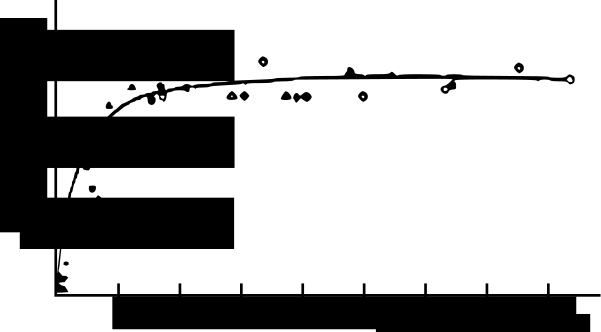
\includegraphics[height=5cm]{./Fig/Chapter1/monod_law}
\caption{
\textbf{Monod law, reproduced from~\cite{monod_growth_1949}.}
Monod has been a pioneer in the formalization of microbial growth into fundamental, coarse-grained relationships.
This figure displays the steady-state growth rate (in number of divisions per hour) of \textit{Escherichia coli} in a synthetic minimal medium at 37$^{\circ}$C containing different concentrations of glucose (a common carbon source).
As the concentration of glucose increases, so does the growth rate of \textit{E.~coli} by following the hyperbolic relationship described in Eq.~\ref{eq:monod_law}.
The solid curve is obtained for $\mu_K = 1.35$ div h\textsuperscript{-1}, and $K_C = 0.22 \cdot 10^{-4}$ mol L\textsuperscript{-1}.
}
\label{fig:monod_law}
\end{figure}

The production of every component of the cell is controlled by a complex network of regulatory interactions.
But an obvious constraint is that at steady state, the synthesis rate of all individual components must be proportional to the growth rate in order to compensate for growth dilution~\cite{monod_growth_1949}.
Many physiological parameters (like the mass of DNA, RNA and protein) are thus functions of the growth rate alone, regardless of the environmental conditions~\cite{schaechter_dependency_1958,bremer_modulation_1996}.
These so-called growth laws were carefully measured~\cite{bremer_modulation_1996} and are still used today in the quantitative understanding of growth control in microorganisms~\cite{ehrenberg_mediumdependent_2012}.
Recently, the topic was revitalized through the work of Scott \textit{et al.}~\cite{scott_bacterial_2011}.
They focused on the ribosome concentration, a physiological parameter that was long known to vary linearly with the growth rate in microorganisms (Fig~\ref{fig:scott_rnaprot}).
By measuring it under different environmental perturbations of the protein synthesis machinery, they built a coarse-grained model describing proteome resource allocation~\cite{scott_emergence_2014}.
It has allowed to show that, whatever the details of the molecular implementation (differing between organisms), this growth law emerges from the underlying principles of robustness and optimization imposed by natural selection, especially growth-rate maximization, in all conditions~\cite{scott_emergence_2014}.

\begin{figure}[tb]
\centering
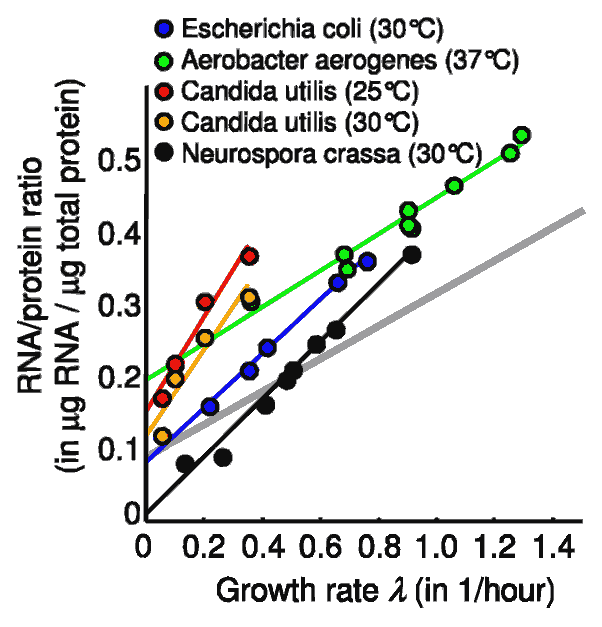
\includegraphics[height=7cm]{./Fig/Chapter1/scott_rnaprot}
\caption{
\textbf{The growth law of ribosomal abundance (figure reproduced from Fig~S1 in~\cite{scott_interdependence_2010}).}
For a variety of carbon sources and their corresponding steady-state growth rate, the RNA/protein ratio is linearly correlated with the growth rate, a relation that holds for many species of microorganisms.
This ratio is correlated with the fraction of ribosome-affiliated proteins, and therefore with the relative abundance of ribosomes in the cell.
}
\label{fig:scott_rnaprot}
\end{figure}

\subsection{Static versus dynamical perspective on growth}

The growth laws cited above apply at steady state, where all intensive properties of the cell are time-invariant~\cite{schaechter_microbe_2006,fishov_microbial_1995}.
This means that the properties that are independent of the cell volume or the cell mass (temperature, concentrations, ...) are constant over time, even though the cell is growing.
It requires that the components of the cell "increase by the same factor over a time interval", which has motivated the use of the term balanced growth~\cite{campbell_synchronization_1957}.
Experimentally, this growth scenario has been used as a standard because it improves reproducibility, in that the results do no longer depend on the precise timing of the samples~\cite{schaechter_microbe_2006}.
It can be easily achieved in the laboratory either in continuous culture, where the substrate is continually supplied~\cite{borirak_molecular_2014}, or in batch conditions if the substrate is in high excess (Fig~\ref{fig:growth_curve}).
This approach has been beneficial to mathematical modeling because considering the system at steady state reduces the complexity of the underlying dynamical system governing microbial growth, allowing genome-scale models encapsulating the enzymatic diversity of living cells to be built and analyzed~\cite{orth_what_2010}.

\begin{figure}[p]
\centering
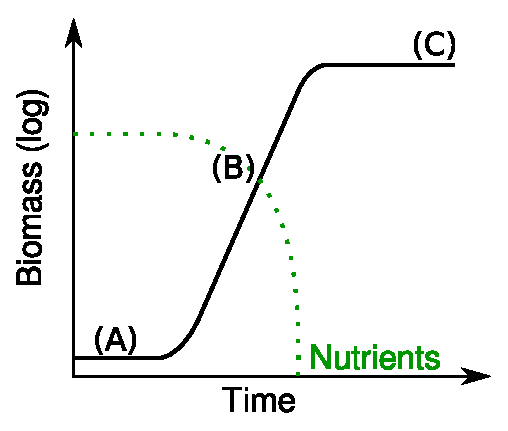
\includegraphics[height=6cm]{./Fig/Chapter1/growth_curve}
\caption{
\textbf{The different phases of a typical growth curve}.
During a typical batch growth scenario, biomass accumulates (black thick line) whereas nutrients are consumed until depletion (green dashed line)~\cite{schaechter_microbe_2006}.
(A) The lag phase is a variable period of time during which the organism adapt to the new medium~\cite{swinnen_predictive_2004}.
It is hard to study experimentaly and is known to be affected by the pre-culturing history of the strain~\cite{ng_damage_1962,dufrenne_effect_1997,shaw_effect_1967}, the magnitude and the rate of the change between the past and present environments~\cite{mcmeekin_predictive_2002}, and other hard-to-control environmental conditions~\cite{cheroutre-vialette_application_2002}.
(B) The steady-state (or balanced-growth) phase is characterized by an exponential production of biomass.
Its characteristics are time-invariant and quite robust accross conditions, which has made it a standard for microbial growth studies~\cite{schaechter_microbe_2006}.
This phase can be extended for hundreds of generations in continuous cultures by the constant renewal of the medium~\cite{borirak_molecular_2014,herbert_continuous_1956,wang_robust_2010}.
As represented here, nutrients are quickly depleted in batch conditions, which does not allow to maintain steady-state growth for a long period of time.
(C) The stationary phase occurs after the depletion of the limiting nutrients in the medium~\cite{chubukov_environmental_2014,schaechter_microbe_2006}.
In natural conditions, microorganisms usually encounter poor media and spend most of their time in stationary phase~\cite{mcarthur_microbial_2006,menge_nitrogen_2012,hobbie_microbes_2013}.
Some species that have evolved long-term resistance mechanisms, like sporulation~\cite{stragier_molecular_1996} or cannibalism~\cite{gonzalez-pastor_cannibalism:_2011}, can survive particularly long stationary phases.
}
\label{fig:growth_curve}
\end{figure}

Although balanced growth is convenient from an experimental and theoretical point of view, it is widely admitted that microorganisms rarely encounter this state in nature~\cite{schaechter_microbe_2006}.
Steady-state growth requires stable conditions over a long period of time, but microorganisms live in
environments where the key elements, such as carbon, nitrogen or phosphorus, are quickly depleted by the competitors as soon as they become available~\cite{mcarthur_microbial_2006,menge_nitrogen_2012,hobbie_microbes_2013}, a consideration that also holds for the lab strains for which growth laws have been established~\cite{savageau_escherichia_1983,savageau_demand_1998,blount_unexhausted_2015,vanelsas_survival_2011}.
Why would microorganisms be optimal for a state they have barely encountered during their evolution?
Are we missing something by studying in stable, unchanging conditions systems that were in fact selected to cope with environmental variations?

\section{Problem statement}
\label{sec:problemstatement}

Microbial growth is essentially a resource allocation problem that can be summarized in simple, fundamental growth laws.
Though established empirically, those laws are elegantly explained if we consider that microorganisms behave in ways that optimize biomass production.
However, these laws describe growth in stable environments and it is hard to imagine how natural selection could have resulted in microorganisms that are optimal for conditions they rarely encounter outside the laboratory.
This motivates the study of growth laws from a dynamical perspective, that is, in a changing environment, and leads us to the following problem statement: \textbf{Which strategies do microorganisms follow in order to dynamically reallocate their resources after a change in the environment?}
The development of this question prompts the following investigations.

What are the best strategies of resource allocation if, like for the steady-state growth laws, we continue to assume that biomass production is the only optimization criterion?
An answer to this question would allow us to assess to which extent the features of dynamical optimization differ from those of steady-state optimization.
In other words, it would test our verbal hypothesis that motivated a dynamical perspective on growth: the expectation that evolutionary pressure applies differently in a changing or stable environment.
In order to achieve this, we need to formulate our problem in mathematical terms, through the development of a proof-of-concept model of resource allocation in bacterial cells, and the theoretical determination of the optimal dynamical allocation of resources following a change in the environment.

The model will help us to establish actual resource allocation strategies that optimize biomass production during an environmental change.
However, it will not be able to tell us if microorganism do actually optimize such a criterion.
We therefore need to measure biomass accumulation and changes in resource allocation following a change in the environment.
How could one measure resource allocation during a growth transition?
In the light of the discussion in the previous section, this requires monitoring the abundance of key macromolecules in living cells over time, while establishing an experimental set-up that allows to control the inherent variability of dynamical experimental studies of microbial growth.

\section{Related work}

\subsection{Modeling growth of microorganisms}

My recent experience as a teacher taught me that, as of today, many students in biology do not like mathematics very much.
Since mathematics is the main language of modeling, this has often made it difficult for me to convince them that modeling is of key importance for biologists.
However, while mathematics is the language, it is not the essence of modeling.
Generally speaking, a model depicts and simplifies reality.
Maps, sketches, or pictures satisfy this definition, as do graphs, sets of equations, or even the DNA sequences stored in a text file on a computer.
In other words, depicting and simplifying reality makes you a modeler, not so much drawing equations on a board.
But this does not change the fact that mathematics are powerful tools for formulating and analyzing models~\cite{servedio_not_2014,mcgill_calm_2013}.

What makes mathematical modeling so useful in microbial growth studies?
%Evolutionary biology is a good example of a field that has relied on mathematical modeling for a long time~\cite{servedio_not_2014}.
%The large time and population scales at which evolutionary processes occur complicate experimental work, despite several attempts on organisms with a short generation time~\cite{barrick_genome_2013,elena_evolution_2003,kassen_experimental_2002,schneider_dynamics_2004}.
%Besides, microbiology is a field particularly prone to experimental study.
%A growth curve as presented in Fig.~\ref{fig:growth_curve} can be made in a day, so the limitations of evolutionary biology should not apply to microbial growth studies.
%But as knowledge and experimental data on microbes accumulates, the need for a systemic understanding of biology is more and more pressing~\cite{alon_introduction_2006,kremling_systems_2013,hillis_why_1993}.
Microbial physiology results from the interplay of thousands of chemical reactions that are not necessarily relevant in any given situation~\cite{schaechter_microbe_2006}.
These reactions occurs on a wide range of time scales (shorter than 1~second for metabolism, to more than 1~day for the degradation of stable proteins~\cite{schaechter_microbe_2006}), and are controlled by several layers of regulatory mechanisms that can only be understood through evolutionary considerations~\cite{dawkins_selfish_1976}.
As a consequence, even the simplest verbal hypothesis can resist direct empirical testing.
But abstracting away complexity is the purpose of mathematical models.
The overwhelming number of variables and the co-existence of several different time scales can be dealt with by choosing the correct framework.
When working on a model, microbial behavior is abstracted into a world of clearly stated rules, where it is easier to spell out the logical consequences of the underlying assumptions~\cite{servedio_not_2014,mcgill_calm_2013}.
Predictions can be made, "unpacked" into our real world, and confronted with experimental testing.

Modeling has proven to be particularly helpful in unveiling how metabolic networks operate.
For an increasing number of microorganisms, we are now able to draw quasi-exhaustive maps of their metabolic reactions.
For instance, a much-used genome-scale reconstruction of \textit{E. coli} metabolism contains 1366 genes, 2251 metabolic reactions, and 1136 unique metabolites~\cite{orth_comprehensive_2011}.
The number of variables may seem overwhelming, and making sense of this information is not straightforward.
Which reactions are important, and in which environmental conditions?
Can we predict how perturbations will affect a given metabolic network?
Do fundamental regularities exist between different metabolic networks, from different species?

The complexity of the reconstructed metabolic networks does not impede their mathematical study.
Constraint-based modeling is a framework that abstracts away the unknown kinetics and represents the metabolic reactions by steady-state fluxes to which physico-chemical constraints can be applied, e.g., compartmentalization, mass conservation, molecular crowding, and thermodynamic directionality~\cite{ebrahim_cobrapy_2013}.
From a mathematical point of view, the model consists of a system of linear equations defining a space of admissible flux distributions that is further reduced by the above-mentioned constraints, which eliminate flux distributions that are unlikely to occur in an environmental condition of interest.
The solution space is often further reduced by selecting the flux distributions optimizing a specified objective function, such as the growth rate of the cell.
This approach, called flux balance analysis (FBA)~\cite{orth_comprehensive_2011,palsson_systems_2011}, has been shown to correctly predict many behaviors of the metabolic network of \textit{E. coli}~\cite{varma_stoichiometric_1994,edwards_silico_2001}.
It has also proved capable of predicting its long-term adaptation through evolution of the network after a gene deletion~\cite{fong_metabolic_2004}.

More direct modeling approaches, in the form of large kinetic models, have also been helpful for understanding growth-related processes.
Through the construction of a model of 47 differential equations and 193 parameters, Kotte \textit{et al.} have shown how metabolic fluxes are sensed at different locations in central carbon metabolism, and are integrated in a global cellular response by the coupling of enzymatic and transcriptional regulation~\cite{kotte_bacterial_2010}.
Kinetic models of this type are sufficiently detailed to be used as an \textit{in silico} testbed to investigate specific molecular mechanisms and uncover their function in bringing about a cellular response~\cite{peskov_kinetic_2012}.
The most emblematic instance of this approach is probably the recent whole-cell model of \textit{Mycoplasma genitalium}~\cite{karr_whole-cell_2012}.
By aggregating all the available knowledge from more than 900 publications, Karr \textit{et al.} constructed a dynamical model accounting for all the annotated gene functions of this pathogenic organism, and successfully used it to investigate unobserved molecular mechanisms and guide novel experimental analysis.
While such approach is not yet applicable to many organisms, it genuinely demonstrates how the increase in computational power could one day guide \textit{in silico} experimentation.

The granularity of the kinetic models cited above is their strength, but also their main weakness.
Despite the available knowledge of molecular mechanisms, precisely measuring \textit{in-vivo} kinetic parameters still represents a technological bottleneck~\cite{park_metabolite_2016,bennett_absolute_2009,buscher_cross-platform_2009}.
While parameter values can be collectively fitted to available data~\cite{jaqaman_linking_2006,mendes_non-linear_1998}, this is known to often produce large parameter uncertainty~\cite{cho_experimental_2003,brodersen_characterization_1987,rodriguez-fernandez_hybrid_2006}.
This is problematic, because the predictions are often particularly sensitive to the parameter values~\cite{gutenkunst_universally_2007,ingram_network_2006,mayo_plasticity_2006}.
Constraint-based modeling overcomes this limitation by using a mathematical approach that does not require any knowledge about the reaction kinetics.
The drawback is that this approach strongly depends on the constraints used to reduce the space of admissible solutions, e.g. the choice of the objective function that may be tricky, as discussed above~\cite{kauffman_advances_2003}.

The limitations of constraint-based and detailed kinetic models have motivated the construction of simpler, coarse-grained models.
The philosophy is quite different: instead of aggregating all available knowledge into a detailed model, the modeler is concerned about carefully filtering this information to keep the model as simple as possible.
The resulting models generally describe cellular functioning on a high level of abstraction, and are particularly valuable when looking for universal laws or principles~\cite{scott_bacterial_2011,scott_interdependence_2010,scott_emergence_2014}.
They can take the form of minimal core models that focus on a given aspect of growth, while still abstracting away the molecular details (see \textit{e.g.}, ~\cite{spiesser_size_2012}).
They can also be used as proof-of-concepts to submit verbal hypotheses to the logic and rigor of mathematical reasoning~\cite{servedio_not_2014}.
For instance, a simple proof-of-concept model was used to uncover the principles leading to overflow metabolism, a mechanism by which microorganisms switch to inefficient metabolic pathways when growing at high nutrient availability~\cite{molenaar_shifts_2009}.
This paradoxical and widespread phenomenon~\cite{dijken_kinetics_1993,vemuri_overflow_2006,mckeehan_glycolysis_1982,hsu_cancer_2008} was shown to be easily explained by the fact that high yield pathways also require the synthesis of more enzymes, revealing the occurrence of a cost-benefit trade-off producing the switch when nutrients are no longer the limiting factor.
Overall, these models have several advantages for the purpose of our study: they clearly state the underlying assumptions, and are sufficiently tractable to be analyzed by a variety of mathematical tools.

%It is also the preferred approach when one wants to broaden its access to mathematical tools~\cite{vandenberg_optimal_1998}, most of them being unhelpful with the high dimensionality of biological models.
%As we will describe in section~\ref{sec:approach}, this represents the modeling strategy that was used in this thesis.

%\begin{figure}[tb]
%\centering
%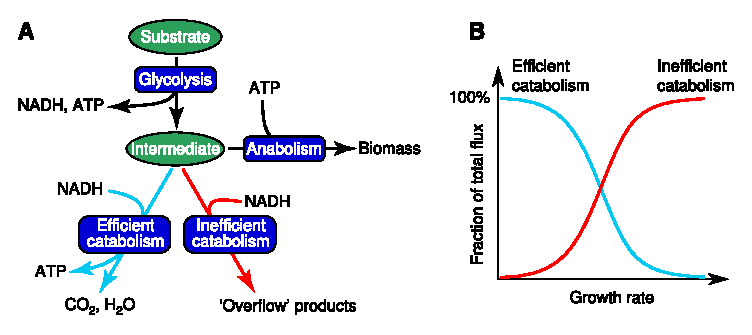
\includegraphics[width=\textwidth]{./Fig/Chapter1/molenaar_overflow.eps}
%\caption{
%\textbf{The strategy of overflow metabolism, reproduced from~\cite{molenaar_shifts_2009}.}
%When increasing the concentration of substrate, the metabolism of microorganisms switches toward the use of inefficient pathways.
%This paradoxical behavior does in fact maximize the growth rate if we take into account the costs and benefits of enzyme synthesis, in particular the fact that pathways for inefficient catabolism are shorter and therefore cheaper to produce.
%(A) Simple view of microbial metabolism, with the two competing efficient and inefficient pathways.
%(B) The switching from efficient to inefficient catabolism when the concentration of nutrients, and hence the growth rate, increases.
%}
%\label{fig:molenaar_overflow}
%\end{figure}

\subsection{Measuring growth of microorganisms}

Either to formulate hypotheses or test predictions, data on microbial growth need to be acquired.
The most straightforward method is to work at the population level.
When working with microorganisms, a clonal population of genetically identical cells can easily be obtained by inoculating a single colony into a growth medium~\cite{schaechter_microbe_2006}.
Over time, this culture can be subjected to different types of measurements: for instance, biomass can be estimated  directly through measurements of the dry weight of samples~\cite{monod_growth_1949}, or indirectly through measurements of transmitted or scattered light across the culture~\cite{volkmer_condition-dependent_2011}, allowing to construct growth curves as presented in Fig.~\ref{fig:growth_curve}.
Other population-wide parameters, like the macromolecular composition~\cite{scott_interdependence_2010,scott_bacterial_2011} or the concentration of metabolites~\cite{bennett_absolute_2009} can also be evaluated.
They represent averaged estimates from billions of genetically identical cells and are thus usually robust and reliable measurements.
In fact, most of \textit{E.~coli} parameters that are currently used in today's growth models have been measured at the population level, notably through the emblematic work of Bremer and Dennis~\cite{churchward_macromolecular_1982,bremer_modulation_1996,bremer_free_2003,bremer_feedback_2008}.

Nevertheless, some questions cannot be solved at the population level~\cite{davey_flow_1996,bakshi_superresolution_2012,balaban_bacterial_2004}.
One example are questions about the internal structure of the cell~\cite{bakshi_superresolution_2012}.
Bakshi \textit{et al.} used a combination of fluorescent labeling and superresolution imaging to localize the ribosomes, RNA polymerases and DNA in living \textit{E.~coli} cells~\cite{bakshi_superresolution_2012}.
They showed that despite what was previously thought, most of the translation occurs far from the DNA, on free mRNA molecules that migrate to ribosome-rich regions~\cite{bakshi_superresolution_2012}.
Another example concerns questions about single-cell variability~\cite{balaban_bacterial_2004,booth_stress_2002,sumner_phenotypic_2002}.
Through growth and imaging of single cells in a microfluidic device, Balaban \textit{et al.} showed that a clonal bacterial population can profit from a preexisting heterogeneity to persist when challenged by the presence of an antibiotic, a short-term mechanism that does not involve any genetic mutation~\cite{balaban_bacterial_2004}.
In the long term, heterogeneity has also been shown to help subpopulations to resist lethal stresses, leaving them with enough time to adapt and conquer new ecological niches~\cite{booth_stress_2002,sumner_phenotypic_2002}.
In fact, cell heterogeneity seems so crucial for the fitness of microorganisms that diversity-generating mechanisms have been identified~\cite{true_yeast_2000,fraser_noise_2004,raser_control_2004}.

In addition to the level of measurement, the cultivation method plays a significant role in the kinds of question that an experiment can answer.
With the advent of molecular genetics in the 1970s and 1980s, batch growth conditions have been the preferred choice of most microbiologists~\cite{hoskisson_continuous_2005}.
As illustrated in Fig.~\ref{fig:growth_curve}, the organism is inoculated in a closed-system and grows until the nutrient is depleted.
In a sense, such a condition is close to what microbes encounter in nature, where key nutrients are only available for a short time and quickly depleted~\cite{mcarthur_microbial_2006,menge_nitrogen_2012,hobbie_microbes_2013}, and is essential to study many questions, \textit{e.g.} diauxic growth~\cite{kremling_understanding_2015}.
Currently, a strong advantage of batch culturing is the intense parallelization that can be attained using microplates.
Indeed, microplates allow to perform dozens to hundreds of growth experiments, each in less than one milliliter, while the optical density or the fluorescence of each culture is automatically monitored.
This has proven extremely helpful for screening purposes and the establishment of standard libraries of gene labeling and modification~\cite{baba_construction_2006,zaslaver_comprehensive_2006}.
Parallel cultivation has notably been exploited to construct roughly 4,000 single-cell knock-out mutants of \textit{Escherichia coli}, forming the Keio collection~\cite{baba_construction_2006}.
This mutant collection was extensively used during the last decade to unveil unknown gene functions and test genome-wide effects of gene deletions (as of 2009, more than 4~millions samples issued from this collection had been shared worldwide~\cite{yamamoto_update_2009}).
Microplates have also helped building a massive library of transcriptional fusions of the green fluorescent protein to each of about 2,000 different promoters in \textit{E.~coli}~\cite{zaslaver_comprehensive_2006}.
Interestingly, microplate batch growing conditions have also been used when applying the above constructions in the inference and analysis of gene regulatory networks~\cite{gerosa_dissecting_2013,berthoumieux_shared_2013,keren_promoters_2013,
ronen_assigning_2002,stefan_inference_2015}.
But the latter use can be hazardous, because the main drawback of the batch condition is that the culturing system is poorly controlled.
Changes of key chemical parameters (\textit{e.g.} pH, pO\textsubscript{2}) have been shown to occur during the whole growth curve~\cite{bekker_changes_2007}. 
At high density, metabolic by-products can accumulate in the medium and impede growth before nutrients are exhausted~\cite{ackerman_accumulation_1974,lenski_chemical_2002,luli_comparison_1990}.
This could be dealt with by focusing on the beginning of the culture, but this part has been shown to strongly depend on the preculture history~\cite{ng_damage_1962,dufrenne_effect_1997,shaw_effect_1967}, and one is never sure when an internal steady state has been reached~\cite{myers_culture_1944}.
%[NB THE FACT THAT CULTURE CONDITIONS CHANGE IS NOT NECESSARILY "HAZARDOUS", IF ALL MEASUREMENTS USED FOR THE INFERENCE PROCESS HAVE BEEN OBTAINED UNDER THE SAME CONDITIONS. THE CHANGE IN CONDITIONS IS ALSO A PERTURBATION OF THE NETWORK AND POSSIBLY INFORMATIVE...]
% Nils: Indeed, but I need to make a point here in order to motivate why we used complicated culture.

For this reason, continuous cultures were developed for microbial studies~\cite{myers_culture_1944,novick_experiments_1950,herbert_continuous_1956}.
Through the permanent renewal of the growth medium, continuous cultures allow for maintenance of a chemically well-controlled environment, allowing for the acquisition of reproducible and reliable data~\cite{borirak_molecular_2014,hoskisson_continuous_2005}.
This has shown to be particularly valuable for comparative omic analysis, for instance the analysis of changes in protein levels~\cite{kolkman_comparative_2005} or genome-wide transcriptomic changes~\cite{boer_genome-wide_2003} that occur when \textit{Saccharomyces cerevisiae} is grown in different media.
Continuous cultures are more difficult to set-up, however~\cite{novick_experiments_1950,borirak_molecular_2014}.
Even if the working volume can be reduced~\cite{betts_miniature_2006}, they usually consume large quantities of medium and are, by design, expected to be more prone to contamination~\cite{novick_experiments_1950}.
But recent advances in microfluidic technology have made it possible to set up robust continuous cultures experiments on the microliter scale~\cite{wang_robust_2010,balaban_bacterial_2004}.
For instance, the mother machine~\cite{wang_robust_2010} allows to perform long-term growth of microorganisms
in continuous culture using only a few milliliters of fresh medium per hour.
This has enabled to show that \textit{E.~coli} growth is remarkably stable on the long term and rather immune to the aging mechanisms that normally affect mother cells in other microorganisms.
It is however important to note that at those scales, growth can only be monitored through microscopy analysis, which could unnecessarily complicate studies that do not rely on single-cell measurements.

The experimental approaches briefly reviewed above can be applied to study microbial growth in a dynamical setting~\cite{levy_strategy_2007,levy_coordination_2009,madar_promoter_2013,ehrenberg_mediumdependent_2012}.
For instance, Levy \textit{et al.}~\cite{levy_strategy_2007,levy_coordination_2009} applied pulse-like environmental perturbations to a continuous culture of yeast, and measured how transcriptomic reorganization occurs.
They observed that the transcription levels are affected before the growth rate of the organism, suggesting a significant role of feed-forward sensing from the environment.
Madar \textit{et al.}~\cite{madar_promoter_2013} analyzed the transcriptional reorganization occuring in \textit{E.~coli} during the lag phase through the coupling of batch experiments in microplates and single-cell measurements \textit{via} flow cytometry.
They showed that \textit{bottleneck enzymes} were produced early in the lag phase, before the cells actually switch to the production of ribosomes and general metabolic enzymes.
As in this PhD project, the studies cited above investigate questions that can only be answered in a dynamical context and they inspired the search for the most appropriate experimental approaches to answer the problem set out in Section~\ref{sec:problemstatement}.
By taking the best of the works presented above, a part of our study will focus on establishing such experimental conditions.

\section{Approach}
\label{sec:approach}

Throughout this study, we focus on a specific dynamical growth scenario, namely the case of a nutrient upshift~\cite{ehrenberg_mediumdependent_2012,kjeldgaard_kinetics_1961,schaechter_patterns_1961,johnsen_control_1977}.
Contrary to steady-state growth, nutrient upshifts and downshifts are frequently encountered in the life cycle of microorganisms~\cite{schaechter_microbe_2006,mcarthur_microbial_2006,menge_nitrogen_2012,hobbie_microbes_2013}.
In combination, they also provide a good approximation of more complex environments.
In nature, nutrient upshifts generally start from stationary phase~\cite{mcarthur_microbial_2006,menge_nitrogen_2012,hobbie_microbes_2013}, a state in which complex adaptive mechanisms are at work that we would like to sidestep for this study~\cite{stragier_molecular_1996,gonzalez-pastor_cannibalism:_2011,ng_damage_1962,dufrenne_effect_1997,shaw_effect_1967,mcmeekin_predictive_2002,cheroutre-vialette_application_2002}.
For this reason, we confine the problem to the study of resource allocation during a so-called steady-state-to-steady-state transition.
While we expect the starting and ending conditions to be on the growth law presented in Fig.~\ref{fig:scott_rnaprot}, we currently have no idea of what happens in the time between.

We start by developing in Chapter~\ref{chap:theory} a simple proof-of-concept model of resource allocation that evaluates how biomass production can be maximized during an upshift from a medium with low nutrient content to a medium with high nutrient content.
The model is an instance of a self-replicator model~\cite{molenaar_shifts_2009}, but focuses on the allocation of resources to only two sectors of the microbial cell: metabolism, taking up and converting nutrients to precursor metabolites, and gene expression, producing macromolecules from the precursors.
The model is kept as simple as possible in order to make sure it stays mathematically tractable in a dynamical context.
A necessary step is however to verify that, at steady-state, the model account for known growth laws of resource allocation~\cite{scott_interdependence_2010,scott_bacterial_2011}.

Using this model, we pose the problem of dynamical optimization as an optimal control problem~\cite{stengel_optimal_1994}.
To comply with what we know at steady state, the microbial cells are assumed to maximize biomass production, but we adapt the criterion to the dynamical context of an upshift scenario.
By using a combination of analytical~\cite{carlson_infinite_1991} and numerical optimization~\cite{bonnans_bocop_2012}, we aim to identify a mathematical upper bound for the biomass produced~\cite{stengel_optimal_1994}.
This theoretical solution can then be used to explore possible regulatory strategies.
In particular, we use the bang-bang~\cite{stengel_optimal_1994} control solution found as a benchmark to identify the system variables that need to be sensed in order to optimize resource allocation.
This provides a common scale on which the outcomes of different regulatory schemes can be compared during an upshift scenario.
This allows us to identify one or several strategies that clearly outperform all the others, giving us testable predictions.
Specifically, we show that feedback from the intracellular state turns out to be much more valuable than information from the environment.
We investigate if such a strategy could be active in real cells, and identify the widespread ppGpp system~\cite{bosdriesz_how_2015} as a possible molecular implementation that could control the synthesis of ribosomes in a switch-like manner during a nutrient upshift.
Overall, this chapter demonstrates that, if microbial cells actually optimize their biomass production during an upshift, they should dynamically allocate their resources to the gene expression machinery in an on-off manner, making an experimentally testable prediction.

In Chapter~\ref{chap:experiments}, we address the challenging problem of experimentally verifying this prediction in \textit{Escherichia coli}.
This task requires the development of an experimental set-up allowing the measurement of resource allocation in our dynamical growth scenario, \textit{i.e.} a steady-state-to-steady-state nutrient upshift.
From the model developed in Chapter~\ref{chap:theory}, we identified that the predicted on-off pattern should occur on a short time scale after the transition (a couple of generations).
This motivates the use of \textit{in-vivo}, high-frequency, single-cell measurements of the concentration of the gene expression machinery.
Inspired by the work of Bakshi \textit{et al.}~\cite{bakshi_superresolution_2012}, we constructed a strain with a GFP-tagged S2 ribosomal subunit, grew this strain in the mother machine, and monitored expression of the reporter gene using fluorescence microscopy~\cite{wang_robust_2010}.
While originally developed for studies of long-term steady-state growth, we used the mother machine here to perform an instantaneous medium transition in a controlled manner from acetate (a poor carbon source) to glucose (a rich carbon source), in order to obtain a significant difference in growth rates between the two media~\cite{andersen_are_1980}.

After segmentation and cell tracking, this set-up was able to generate fluorescence and size time series for dozens of cells.
Using again the self-replicator model as a framework, we showed that these measurements are sufficient for the intended signal reconstructions, in particular the growth rate and the resource allocation profile over time.
The method we used is called Kalman smoothing~\cite{kailath_linear_2000,jazwinski_stochastic_2007}.
While well-known in engineering, Kalman smoothing has been rarely used in quantitative biology, but turned out to be particularly suitable for the purpose of the model-based analysis of gene expression data in single cells, as we argue and show on synthetic data in Chapter~\ref{chap:experiments}.
Finally, the experimental verification or falsification of the optimal control prediction, should allow to conclude whether the biomass maximization, as considered in Chapter~\ref{chap:theory}, is indeed a cell objective in a dynamical context.

\chapter{Dynamical Allocation of Cellular Resources as an Optimal Control Problem: Novel Insights into Microbial Growth Strategies}
\chaptermark{Dynamical allocation of cell resources}
\label{chap:theory}

\textit{Rather than propose a new theory or unearth a new fact, often the most important contribution a scientist can make is to discover a new way of seeing old theories or facts.} -- Richard Dawkins, \textit{The Selfish Gene}~\cite{dawkins_selfish_1976}, preface to 1989 edition.

\begin{center}
\noindent\rule{4cm}{0.1pt}
\end{center}

\selectlanguage{french}
\begin{chapter_summary}{Modélisation de l'allocation dynamique des ressources cellulaires comme un problème de contrôle optimal}

Ce chapitre est dédié à une approche théorique du problème d'allocation des ressources cellulaires chez les microorganismes.
En Section \ref{sec:model}, nous modélisons la cellule comme un auto-réplicateur devant allouer une ressource commune (les nutriments du milieu) à deux secteurs distincts de macromolécules: la machinerie métabolique qui extrait les nutriments de l'environnement et les convertit en précurseurs utilisables, et la machinerie d'expression génique qui utilise ces précurseurs pour produire de nouvelles macromolécules (Fig.~\ref{fig:self_replicator}).
Ce modèle très simple comprenant 2 réactions (Eq.~\ref{eq:reactions}) se traduit mathématiquement par deux équations différentielles ordinaires (Eqs~\ref{eq:pdef} et \ref{eq:rdef}) faisant intervenir le paramètre $\alpha$ qui va devenir clé dans notre étude.
$\alpha$ représente la proportion massique des précurseurs qui sont utilisés pour produire de la machinerie d'expression génique, au détriment de la machinerie métabolique (qui elle, est produite à la proportion $1-\alpha$).
Comme on l'a déjà vu avec les lois de croissance établie à l'état stationnaire (voir Chapitre~\ref{chap:introduction}), cette proportion varie avec l'environnement, on s'attend donc à ce que $\alpha$ en fasse autant, augmentant d'autant que l'environnement devient riche (Fig.~\ref{fig:scott_rnaprot}).
Cependant, de quelle manière varie-t-il entre deux états de croissance stationnaire, lorsque les composants cellulaires sont en déséquilibre et que la cellule doit adapter sa composition ?

Comme nous l'avons vu dans le Chapitre~\ref{chap:introduction}, les lois de croissances à l'état stationnaire s'expliquent facilement si l'on considère que la cellule maximise son taux de croissance.
En Section~\ref{sec:growthlaws}, nous voyons en effet que pour chaque environnement, un $\alpha$ unique existe qui maximise la croissance de la cellule, mais surtout que ce $\alpha^*_{opt}$ est d'autant plus important que l'environnement est riche (Fig.~\ref{fig:model_analysis}).
De fait, les lois de croissances à l'état stationnaire sont parfaitement prédites par notre modèle simple en considérant uniquement que la cellule maximise son taux de croissance (Fig.~\ref{fig:model_validation}).
Peut-on appliquer le même principe, dans un contexte cette fois dynamique, de façon à prédire comment la cellule distribue ses ressources lors d'une transition de croissance ?

Dans ce contexte, $\alpha$ est désormais une fonction du temps.
Nous cherchons donc quelle fonction du temps maximise un objectif donné.
Ce problème, formulé en Section~\ref{sec:optimalcontrolproblem}, est un problème de contrôle optimal, puisque l'objectif à optimiser est une fonction d'une autre fonction, plus communément appelée fonctionnelle.
Nous choisissons comme équivalent dynamique de la maximisation du taux de croissance à l'état stationnaire, la maximisation de la production de biomasse sur un intervalle de temps comprenant un changement abrupt de l'environnement (Eq.~\ref{eq:biomassdyn}).
Nous résolvons ce problème en Section~\ref{sec:optimalcontrolsolution} en couplant utilisation du principe du maximum de Pontryagin avec de l'optimisation numérique.
La solution optimale obtenue montre que le contrôle $\alpha$ doit prendre alternativement les valeurs 0 ou 1 jusqu'à ce que le système soit stabilisé sur un nouvel équilibre (Fig.~\ref{fig:optimalcontrol} et Eq.~\ref{eq:optcontrol}).
En d'autres termes, la meilleure production de biomasse s'obtient si, à tout moment, la cellule aiguille 100\% de ses ressources vers un seul secteur, en alternant entre l'un et l'autre jusqu'à ce que le nouvel état stationnaire de croissance soit atteint.
Ce type de solution se rencontre souvent en contrôle optimal, et répond au nom de concept TOR (Tout-Ou-Rien, ou \textit{bang-bang-control} en anglais).
Mais ce contrôle est-il pertinent d'un point de vue biologique ?
La cellule a-t-elle suffisamment d'information à sa disposition pour réaliser une telle transition, laquelle repose sur des changements abrupts de l'expression génique à des instants bien précis ?

En Section~\ref{sec:steadystate}, nous utilisons le problème de contrôle optimal et sa solution comme un banc d'essai permettant de comparer entre elles différentes stratégies de régulations (Fig.~\ref{fig:strategies_overview}).
En se servant du modèle pour guider notre intuition, et en nous limitant aux solutions qui respectent les lois de croissance stationnaire, nous montrons que deux stratégies de régulations simples sont possibles : soit l'organisme mesure directement la quantité de nutriments dans l'environnement, soit il mesure la concentration en précurseurs dans la cellule.
De manière intéressante, ces deux stratégies sont optimales à l'état stationnaire, et donc strictement équivalentes.
Cependant, dans le contexte dynamique de notre banc d'essai, la stratégie qui consiste à mesurer les précurseurs est bien plus efficace, même si elle reste évidemment inférieure à la solution optimale (Fig.~\ref{fig:comparison_nutrients_precursor}).

Finalement, nous montrons en Section~\ref{sec:strategies} qu'une stratégie plus complexe mesurant à la fois les précurseurs et la concentration en machinerie d'expression génique est tout à fait capable de réaliser un contrôle proche du tout-ou-rien optimal (Eq.~\ref{eq:stratswitch} et Fig.~\ref{fig:onoffresults}).
Mais surtout, en réutilisant un modèle du système ppGpp, connu pour réguler la synthèse des ribosomes chez la bactérie \textit{Escherichia coli}, nous montrons que ce système répond, au moins structurellement, aux exigences d'une telle stratégie de régulation (Fig.~\ref{fig:ppGppsurface}).
Cela procure un nouveau point de vue sur ce système, d'ailleurs largement répandu chez de nombreux microorganismes.
En intégrant l'information provenant à la fois de la quantité de ribosomes et de celle des précurseurs, il permet d'allouer efficacement les ressources de la cellule lorsque celle-ci doit s'adapter rapidement à un nouvel environnement.
\end{chapter_summary}
\selectlanguage{english}

\begin{center}
\noindent\rule{4cm}{0.1pt}
\end{center}

\section*{Beginning of Chapter \thechapter}

\noindent \textbf{Important note:} Text and figures in this chapter have been published in Plos Computational Biology~\cite{giordano_dynamical_2016} under the terms of the \href{https://creativecommons.org/licenses/by/4.0/}{Creative Commons Attribution License} (CC-BY 4.0).

%%%%%% CORE OF THE ARTICLE %%%%%
\section{Introduction}

Microorganisms adapt their physiology to changes in nutrient availability in the environment.
This involves changes in the expression of a large number of genes, encoding proteins with a variety of cellular functions, such as transporters for the uptake of nutrients, enzymes for the conversion of nutrients to energy and building blocks for macromolecules, the components of the transcriptional and translational machinery, and transcription factors to preferentially direct RNA polymerase to specific promoters~\cite{schaechter_microbe_2006,keseler_ecocyc_2013}.
Fundamentally, the reorganization of gene expression in response to changes in environmental conditions is a resource allocation problem.
It poses the question how microorganisms redistribute their protein synthesis capacity over different cellular functions when constrained by the changing environment.

The mechanisms responsible for resource allocation in microbial cells are usually assumed to have been optimized through evolution, so as to maximize the offspring of cells in their natural environment.
How this general principle manifests itself on the level of cellular physiology is not straightforward though.
Many studies have reasoned that growth-rate maximization provides a selective advantage to microorganisms, because it allows competitors to be outgrown when resources are scarce.
Others have shown, however, that appropriate optimization criteria will depend on the structure of the environment and the ecosystem, as well as on the molecular properties of metabolic pathways~\cite{frank_tradeoff_2010,maclean_tragedy_2008,schuetz_multidimensional_2012,schuster_maximization_2008,schuetz_systematic_2007}.
For instance,  in environments without competition for a shared resource, maximization of growth yield rather than growth rate is expected to provide a selective advantage.
Although what counts as optimal is thus context-dependent, growth and evolution experiments in \textit{Escherichia coli} have shown that in certain conditions bacterial metabolism is indeed geared towards growth-rate maximization~\cite{edwards_silico_2001,ibarra_escherichia_2002,lewis_omic_2010}.

For this reason, growth-rate maximization is a central hypothesis in a number of recent theoretical studies of resource allocation using coarse-grained models of the cell~\cite{molenaar_shifts_2009,scott_interdependence_2010,scott_emergence_2014}.
The models deliberately reduce the molecular complexity of regulatory networks so as to focus on generic explanatory principles~\cite{servedio_not_2014}.
Along these lines, Molenaar \textit{et al.} developed a series of simple models of the microbial cell, taking into account that growth requires the synthesis of proteins playing a role in metabolism (transporters, enzymes) and gene expression (ribosomes), in varying proportions.
Allocation parameters that maximize the growth rate were shown to account, at least in a qualitative way, for the variation of the amount of ribosomal protein as a fraction of total protein in different growth media, and for the occurrence of overflow metabolism above certain growth rates~\cite{molenaar_shifts_2009}.
Using another coarse-grained model of the cell, centered on amino acid supply (metabolism) and demand (protein synthesis), Scott \textit{et al.} derived empirical growth laws with linear relations between the ribosomal protein fraction and the growth rate, in conditions where the nutrient supply or demand are altered~\cite{scott_interdependence_2010,scott_emergence_2014}.
In their model, maximization of growth rate requires maximization of amino acid flux and is achieved for a specific, unique value of the ribosomal protein fraction.
Based on a structurally similar model, Maitra and Dill related optimal resource allocation to the basic constants of the metabolic and gene expression machinery, in particular energy efficiency~\cite{maitra_bacterial_2014}.

The assumption of growth-rate maximization may lead to correct predictions in some situations, but ignores the regulatory mechanisms achieving resource allocation and therefore cannot provide a causal explanation of cellular behavior~\cite{kremling_understanding_2015}.
Several studies have used coarse-grained models to understand which control strategies microorganisms employ to achieve (optimal) resource allocation~\cite{bosdriesz_how_2015,scott_emergence_2014,weisse_mechanistic_2015}.
Scott \textit{et al.} have shown that a robust feedforward control strategy, based on the sensing of the amino acid pool size and the corresponding adjustment of the fraction of ribosomes producing ribosomal proteins, allows the ribosomal protein fraction to be maintained close to its optimal value under a variety of growth conditions~\cite{scott_emergence_2014}.
The authors suggest that this control strategy involves the signalling molecule ppGpp, in agreement with conclusions drawn from a recent kinetic model of the regulatory mechanisms achieving optimal adjustment of the ribosomal protein fraction~\cite{bosdriesz_how_2015}.
Wei{\ss}e \textit{et al.} also developed a coarse-grained model of microbial growth based on resource allocation trade-offs~\cite{weisse_mechanistic_2015}. 
Without including specific regulatory interactions, the model accounts for the above-mentioned bacterial growth laws, predicts host-circuit interactions in synthetic biology, and relates gene regulation to the nutrient composition of the medium.

The above studies consider resource allocation at steady state, where all intensive variables describing the growing microbial culture, in particular the concentrations of its molecular components, are constant (see~\cite{fishov_microbial_1995} for a precise definition of steady-state growth and the closely related notions of balanced and exponential growth).
This requires an environment to be stable over a long period of time.
Such conditions can be achieved in the laboratory~\cite{borirak_molecular_2014}, but many microorganisms naturally experience frequently-changing conditions.
For example, \textit{E. coli} can cycle between two distinct habitats, the mammalian intestine and the earth's surface (water, sediment, soil)~\cite{savageau_escherichia_1983}.
The bacteria transit through different microenvironments in the intestinal system, where they encounter different mixes of sugars~\cite{savageau_demand_1998}.
They are even more challenged in the open environment outside the host, with a greatly fluctuating availability of carbon and energy sources and a large variability in temperature, osmolarity, oxygen, and microbial communities~\cite{blount_unexhausted_2015,vanelsas_survival_2011}.

This situation motivates a dynamical perspective on microbial growth and resource allocation~\cite{pavlov_optimal_2013,vandenberg_optimal_1998,waldherr_dynamic_2015,ehrenberg_mediumdependent_2012}. However, fundamental results like the growth laws uncovered for steady-state conditions are still lacking.
In particular, extending the results reviewed above to dynamical conditions raises the following questions:
Are control strategies that maximize steady-state growth also optimal in dynamical environments?
If this is not the case, then which alternative strategies would be optimal for such conditions?
And finally, how do these strategies compare with the regulatory mechanisms that have actually evolved in microorganisms?

The aim of this study is to address the above fundamental questions in a specific dynamical growth scenario, namely a transition between two steady states following an environmental perturbation.
In particular, we consider the upshift of a microbial culture from a medium supporting growth at a low rate to a medium supporting growth at a high rate~\cite{ehrenberg_mediumdependent_2012}.
We develop a coarse-grained model of the cell, inspired by the self-replicator model of Molenaar \textit{et al.}~\cite{molenaar_shifts_2009}, and reformulate our questions in the context of optimal control theory~\cite{stengel_optimal_1994} to identify control schemes maximizing biomass production over an interval of time, the dynamical equivalent of growth-rate maximization.

We show that Pontryagin's Maximum Principle suggests that optimal resource allocation after a growth transition is achieved by a bang-bang-singular control law~\cite{stengel_optimal_1994}, a conjecture confirmed by direct numerical optimization.
This optimal solution provides a gold standard against which possible control strategies of the cell can be compared.
We consider simple strategies that drive the system to the steady state enabling growth at the maximal rate in the new medium, after the upshift.
In a dynamical growth scenario, the strategy sensing the concentration of precursor metabolites emerges as the best candidate, consistent with the analysis of Scott \textit{et al.} that feedforward activation of the rate of synthesis of ribosomal proteins, involving ppGpp-mediated sensing of the amino acid pool~\cite{dalebroux_ppgpp_2012,potrykus_pppgpp_2008,hauryliuk_recent_2015}, is the key regulatory mechanism for growth control.
It is possible, however, to define a strategy approaching the theoretical optimum even more closely by exploiting information on both the precursor concentration and the abundance of the gene expression machinery.
Interestingly, a thorough analysis of the functioning of the ppGpp system, as described by a kinetic model of the synthesis and degradation of this signalling molecule, suggests similarities between our two-variable control strategy and the regulation of the transcription of ribosomal RNA by ppGpp~\cite{bosdriesz_how_2015}.

The results presented here generalize the analysis of control strategies enabling optimal growth of microorganisms from steady-state to dynamical scenarios.
The control strategies are formulated in the context of a coarse-grained model of resource allocation, based on minimal assumptions, that accounts for empirical growth laws at steady state.
The analysis shows that during growth transitions, control strategies based on information of a single variable are outperformed by systems measuring several variables.
This conclusion agrees with the intuition that, in dynamical environments, there may be an evolutionary pressure towards more elaborate sensory systems.
From a methodological point of view, our study illustrates how optimal control theory can provide novel insights into complex biological phenomena~\cite{iglesias_control_2010}. 

%%%%%%%%%%%%%%%%%%%%%%%%%%%%%%%%%%%%%%%%%%%%%%%%%%%%%%%%%%%%%%%%%%%%%%%%%%%%%%%%%%%%%%%%%%

\section{Results}

\subsection{Self-replicator model of resource allocation}
\label{sec:model}

Resource allocation in bacteria involves the distribution of cellular resources (precursor metabolites and energy) over processes supporting maintenance and growth~\cite{schaechter_microbe_2006}.
A simple modelling tool for analyzing resource allocation questions in a precise way are so-called self-replicator models.
These models have a long history in various domains of chemistry, biology, physics, and computer science~\cite{sipper_fifty_1998}, and were recently put to use as an analytical tool in systems biology~\cite{molenaar_shifts_2009} (see also~\cite{flamm_minimal_2007}).
We will show that despite their simplicity, which make them tractable for mathematical analysis, self-replicator models are sufficiently expressive to account for empirical observations and make testable predictions.

Bearing in mind that the major constituents of the cell are macromolecules (DNA, RNA, proteins), produced from precursor metabolites, a fundamental resource allocation question is the following: How much of the cellular resources are invested in the making of new macromolecules (gene expression machinery) and how much in performing other functions, in particular producing metabolic enzymes involved in the uptake of nutrients and their conversion to precursor metabolites (metabolic machinery)?
In order to address this question, we consider a self-replicating system composed of the gene expression machinery ($R$) and the metabolic machinery ($M$).
The system, shown schematically in Fig.~\ref{fig:self_replicator}, is thus defined by two macroreactions which are conveniently written as:
\begin{equation}\label{eq:reactions}
\begin{aligned}
S &\overset{V_M}{\longrightarrow} P, \\
P &\overset{V_R}{\longrightarrow} \alpha R + (1-\alpha) M.
\end{aligned}
\end{equation}
The first reaction, catalyzed by $M$, converts external substrates ($S$) into precursor metabolites ($P$).
The second reaction, catalyzed by $R$, converts precursors into macromolecules ($R$ and $M$).
The resource allocation parameter $\alpha \in [0,1]$ defines the proportion of precursor mass used for making gene expression machinery as compared to metabolic machinery.
We will interchangeably use the symbols $M$, $R$, $S$, and $P$ for the components of the replicators themselves and their total mass [g].
We will denote the rates at which the macroreactions occur by $V_R$ and $V_M$ [g~h\textsuperscript{-1}].

\begin{figure}[tb]
\centering
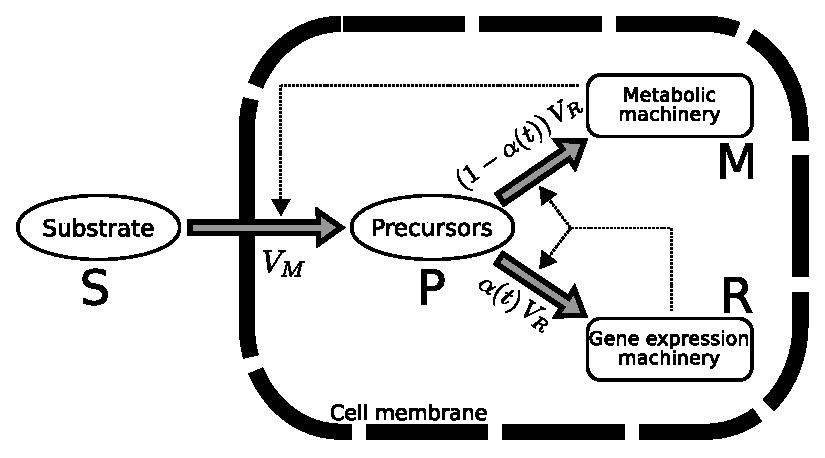
\includegraphics[scale=0.7]{./Fig/Fig1}
\caption{
\textbf{Self-replicator model of bacterial growth.}
External substrates $S$ enter the cell and are transformed into precursors $P$ through the action of the metabolic machinery $M$.
The precursors are used by the gene expression machinery $R$ to make the proteins composing both the metabolic machinery (transporters, enzymes, ...) and the gene expression machinery itself (RNA polymerase, ribosomes, ...).
$\alpha$ ($1-\alpha$) is the mass proportion of precursors converted into $R$ ($M$).
Thick arrows denote reactions and thin, dashed arrows denote catalytic activities.
The rate of synthesis of precursors and the rate of synthesis of proteins from precursors are denoted by $V_M$ and $V_R$, respectively.
}
\label{fig:self_replicator}
\end{figure}

The self-replicator system in Fig.~\ref{fig:self_replicator} is based on a number of simplifying assumptions.
First, cell division is not explicitly modelled and replication should therefore be interpreted as the growth of (the mass of) a cell population.
This amounts to the assumption that individual cells in a growing populations have the same macromolecular composition.
Second, degradation of the macromolecules is ignored.
In other words, we assume that macromolecules are stable and that their degradation rates are negligible with respect to the rates of other reactions in the system.
Third, we consider only two classes of macromolecules ($R$ and $M$).
In particular, we do not assume that an irreducible mass fraction of the precursors is dedicated to cell maintenance~\cite{scott_interdependence_2010}.
The system could be easily extended to relax the above assumptions, but this would complicate the analysis of the model and obscure the points we want to make.

In what follows, it will be more convenient to describe the quantities in the system as intracellular concentrations rather than as the total mass in the cell population.
To this end, we define the volume $\mathtt{Vol}$ [L] of the cell population as follows:
\begin{equation}
\mathtt{Vol} = \beta \, (M + R),
\label{eq:voldef}
\end{equation}
with $\beta$ a conversion constant [L~g\textsuperscript{-1}] equal to the inverse of the cytoplasmic density.
Dividing each variable $M$, $R$, and $P$ by $\mathtt{Vol}$ yields the concentrations $m$, $r$, and $p$ of metabolic enzymes, ribosomes and other components of the gene expression machinery, and precursor metabolites, respectively [g~L\textsuperscript{-1}].
Henceforth, these variables as well as $\mathtt{Vol}$ and $\alpha$ will be considered functions of time $t$ [h].

The dynamics of the self-replicator in Fig.~\ref{fig:self_replicator} can be described by the following system of ordinary differential equations (see \ref{S1_Text} for the derivation):
\begin{eqnarray}
\frac{dp}{dt} &=& v_M(s,r) - v_R(p,r) \, (1+\beta\, p), \label{eq:pdef}\\
\frac{dr}{dt} &=& v_R(p,r) \, (\alpha(t) - \beta\, r), \label{eq:rdef}
\end{eqnarray}
where $s$ [g~L\textsuperscript{-1}] denote the (extracellular) concentration of substrate.
$v_M(s,r)$ [g~L\textsuperscript{-1}~h\textsuperscript{-1}] and $v_R(p,r)$ [g~L\textsuperscript{-1}~h\textsuperscript{-1}] denote the precursor synthesis rate and the macromolecule synthesis rate, respectively.
The growth rate $\mu$ [h\textsuperscript{-1}] of the replicator system is defined as the relative increase of the volume, and can be rewritten with Eqs~\ref{eq:pdef}-\ref{eq:rdef} as proportional to the macromolecule synthesis rate (\ref{S1_Text}):
\begin{equation}\label{eq:growthrate}
\mu = \frac{1}{\mathtt{Vol}} \frac{d\mathtt{Vol}}{dt} = \frac{1}{M+R}\frac{d(M+R)}{dt} = \beta\, v_R(p,r).
\end{equation}

The precursor concentration changes through the joint effect of the precursor synthesis rate $v_M(\cdot )$, the macromolecule synthesis rate $v_R(\cdot )$, and the rate of growth dilution ($\beta\, v_R(\cdot ) \,p$).
The change in concentration of ribosomes and other components of the gene expression machinery is the net effect of the ribosome synthesis rate ($\alpha (\cdot )\, v_R (\cdot)$) and the rate of growth dilution ($\beta \, v_R(\cdot) \, r $).
Remark that it is not necessary to add an equation for $m$ because it follows from Eq.~\ref{eq:voldef} that $r + m = 1/\beta$, and therefore $dm/dt = - dr/dt$.

We use Michaelis-Menten kinetics to define the synthesis rate of each reaction:
\begin{align}
v_M(s,r) &= k_M\,m\, \frac{s}{K_M + s} = k_M\,(1/\beta - r)\, \frac{s}{K_M + s},  \label{eq:metaflux} \\
v_R(p,r) &= k_R\,r\, \frac{p}{K_R + p}, \label{eq:machflux}
\end{align}
with rate constants $k_M, k_R$ [h\textsuperscript{-1}] and half-saturation constants $K_M, K_R$ [g~L\textsuperscript{-1}].
Note that the rate of precursor synthesis is proportional to the concentration of the components of the metabolic machinery, while the macromolecule synthesis rate is proportional to the concentration of the components of the gene expression machinery.
These catalytic effects correspond to the dashed arrows in Fig.~\ref{fig:self_replicator}.
The rate constant $k_M$ depends both on the quality of the nutrients in the medium (higher $k_M$ for a richer medium) and on the metabolic efficiency of the macroreaction converting the substrate into precursors (higher $k_M$ for a more efficient reaction).
For convenience, we henceforth assume that the environmental conditions do not change over the time-interval considered, either because $s$ is constant or because $s \gg K_M$, corresponding to a situation in which the substrate is available in excess.
In both cases, $e_M(s) = k_M\, s/(K_M + s)$ is approximately constant, so that we can write
\begin{equation}
\label{eq:metaflux_simplified}
v_M (r) = e_M \, (1/\beta-r).
\end{equation}
The rate constant $k_R$ characterizes the efficiency of the gene expression machinery, depending on the elongation rate of ribosomes, among other things. The ratio $p/K_R$ is an indicator of the saturation of the gene expression machinery by precursors.

The system of Eqs~\ref{eq:pdef}-\ref{eq:rdef} thus has four parameters ($e_M$, $k_R$, $K_R$, $\beta$), one of which characterizes the input from the environment ($e_M$).
The order of magnitude of the parameters can be inferred from data in the literature, as explained in \ref{S2_Text}.
Below we use the following values for the parameters $e_M = 3.6$~h\textsuperscript{-1}, $k_R = 3.6$~h\textsuperscript{-1}, $K_R=1$~g~L\textsuperscript{-1}, $\beta = 0.003$~L~g\textsuperscript{-1} (\ref{S1_Table}).
However, it should be emphasized that the conclusions of this paper do not depend on the exact quantitative values of these parameters.

An interesting property of the model is that it is built on minimal assumptions, basically the two macroreactions and the definition of the volume as proportional to the total mass of macromolecules.
Like in~\cite{molenaar_shifts_2009,pavlov_optimal_2013,scott_emergence_2014}, these assumptions directly lead to the expression of the growth rate in Eq.~\ref{eq:growthrate}, without additional assumptions.

\subsection{Growth-rate maximization of the self-replicator reproduces bacterial growth laws}
\label{sec:growthlaws}

The nullcline for $r$ is given by $r=0$, $r=\alpha/\beta$, and $p=0$, while the nullcline for $p$ is defined by

\[
r = \frac{e_M}{\beta \left(e_M + k_R\, \frac{p}{K_R+p}\, (1+\beta p)\right)}.
\]
The nullclines define a single stable steady state $(p^*, r^*)$ (Fig.~\ref{fig:model_analysis}\textit{A} and \textit{Methods}).
At this steady state, the growth rate is constant and denoted by $\mu^*$.
The nullcline for $p$ is defined by the environment $e_M$.
The nullcline for $r$, and thus the location of the steady state with the associated growth rate, are given by $\alpha$.
Fig.~\ref{fig:model_analysis}\textit{B} shows the dependency of the steady-state growth rate $\mu^*$ on the resource allocation parameter $\alpha$.
As can be seen, $\mu^*$ is maximal for a specific, unique value of $\alpha$, which we denote $\alpha_{opt}^*$.
That is, the model predicts that there is a single optimal way to divide the precursor flux over the synthesis of the gene expression machinery and the metabolic machinery.
The same result, using a similar model, was obtained by Scott \textit{et al.}~\cite{scott_emergence_2014}.
The self-replicator model is simple enough to derive an algebraic expression for computing $\alpha^*_{opt}$ and the corresponding maximal growth rate $\mu^*_{opt}$ (\textit{Methods} and \ref{S1_Text}), which will simplify analysis of the system in later sections.

\begin{figure}[tb]
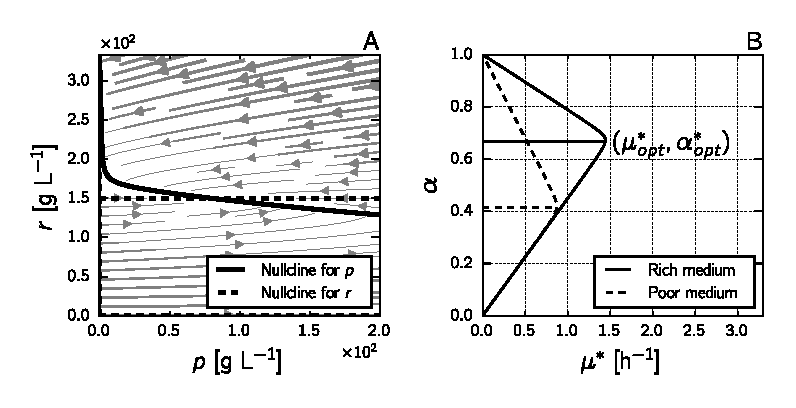
\includegraphics[width=\textwidth]{./Fig/Fig2}
\caption{\textbf{Analysis of self-replicator model of bacterial growth.}
\textit{A:}~Phase-plane analysis of the self-replicator model of Eqs~\ref{eq:pdef} and \ref{eq:rdef}.
The nullclines for $p$ and $r$ are shown as solid and dashed curves, respectively.
Parameter values are $e_M = 3.6$~h\textsuperscript{-1}, $k_R = 3.6$~h\textsuperscript{-1}, $K_R=1$~g~L\textsuperscript{-1}, $\beta = 0.003$~L~g\textsuperscript{-1}, $\alpha = 0.45$.
\textit{B:}~Dependence of the growth rate at steady state $\mu^{*}$ on the resource allocation parameter $\alpha$, for two different environmental conditions (solid line, $e_M = 4.76$~h\textsuperscript{-1}; dashed line, $e_M = 1.57$~h\textsuperscript{-1}, other parameter values are $k_R = 2.23$~h\textsuperscript{-1}, $K_R=1$~g~L\textsuperscript{-1}, and $\beta = 0.003$~L~g\textsuperscript{-1}).
The maximal growth rate is attained for a unique $\alpha$, called $\alpha^*_{opt}$.
}
\label{fig:model_analysis}
\end{figure}

In order to validate the model, we verified that it can account for data on the macromolecular composition of \textit{E. coli} at steady state~\cite{scott_interdependence_2010}.
When optimizing $\alpha$ for different values of $e_M$ (assuming cells attain maximal growth), the model predicts a relation between $\alpha^*_{opt}$ and $\mu^*_{opt}$ (colored dots and black dashed line in Fig.~\ref{fig:model_validation}\textit{A}) that is quasi-linear for high growth rates.
We compared this prediction with the results of experiments where the relation between the growth rate and the mass ratio of total RNA and protein was determined in different growth media (Fig.~\ref{fig:model_validation}\textit{B}).
In the framework of our model, different media correspond to different values of $e_M$, and different total RNA/protein mass ratios to different values of $\alpha$ (up to a conversion factor), allowing a direct comparison of the model predictions in Fig.~\ref{fig:model_validation}\textit{A} with the data in Fig.~\ref{fig:model_validation}\textit{B} (see \textit{Methods}).
As can be seen, the model is able to account for the observed quasi-linear relation between the growth rate and the total mass ratio of RNA and protein. 
Moreover, for realistic values of $k_R$ and $e_M$, a good quantitative fit is obtained (\textit{Methods} and \ref{S1_Table}).

\begin{figure}[p]
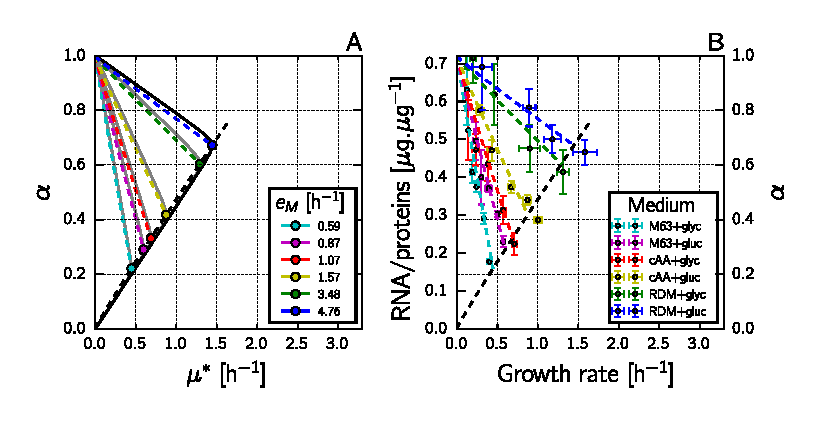
\includegraphics[width=\textwidth]{./Fig/Fig3}
\caption{
\textbf{Self-replicator model accounts for bacterial growth laws.}
\textit{A:}~Predicted quasi-linear relation between the maximal growth rate $\mu^{*}_{opt}$ and the corresponding optimal resource allocation $\alpha^*_{opt}$, for different values of $e_M$ (different colors).
The colored dots indicate $\alpha^*_{opt}$ and $\mu^{*}_{opt}$  for $k_R = 2.23$~h\textsuperscript{-1} and different $e_M$, and the dashed black line the relation for all intermediate values of $e_M$.
The dashed colored lines indicate the relation between $\alpha^*_{opt}$ and $\mu^{*}_{opt}$ obtained when, for a given value of $e_M$, the value of $k_R$ is decreased (lower $k_R$ leads to lower $\mu^{*}_{opt}$).
The solid grey curves correspond to $(\mu^*,\alpha)$-profiles like those shown in Fig.~\ref{fig:model_analysis}\textit{B}.
\textit{B:}~Measured relation between the total RNA/protein mass ratio and the growth rate, in different growth media with different doses of a translation inhibitor (data from~\cite{scott_interdependence_2010}).
For each medium, indicated by a color, five different concentrations of inhibitor were used (higher dose leads to lower growth rate).
Growth-medium compositions are given in the original publication and error bars represent standard deviations.
The dashed black and colored lines are the same as in panel \textit{A}, indicating the good quantitative correspondence between model predictions and experimental data for the chosen parameter values, obtained by fitting the model to the data points (see \textit{Methods} for details).
}
\label{fig:model_validation}
\end{figure}

The data from Scott \textit{et al.} also reveal a second apparently linear relation between the growth rate and the total RNA/protein mass ratio.
This relation is obtained when varying, in the same growth medium, the efficiency of protein synthesis by adding different doses of an inhibitor of translation (chloramphenicol)~\cite{scott_interdependence_2010}.
Using the model, we computed $\alpha^*_{opt}$ and $\mu^*_{opt}$, for constant environment $e_M$ and different values of the efficiency of protein synthesis $k_R$ (dashed colored lines in Fig.~\ref{fig:model_validation}\textit{A}).
As can be seen in Fig.~\ref{fig:model_validation}\textit{B}, the model also captures the second linear relation in the data.

We conclude that the self-replicator model is able to reproduce known observations of resource allocation in bacteria, so-called growth laws~\cite{scott_interdependence_2010}.
The model is similar to a model recently proposed by Scott \textit{et al.}~\cite{scott_emergence_2014}.
Contrary to the latter model, the translation rate is not assumed to be constant in the self-replicator model, but rather depends on precursor abundance, as proposed by the same authors in~\cite{klumpp_molecular_2013}.

The above analysis of bacterial growth has two major limitations.
First, the predictions of optimal resource allocation (the value of $\alpha$ leading to the maximal growth rate) hold at steady state, for a constant environment, whereas most bacteria are not expected to encounter such conditions outside the laboratory.
An allocation of resources that is optimal for steady-state growth and constant over time may not be optimal in dynamical growth conditions.
Second, while it predicts which value of $\alpha$ is optimal at steady state, the model says nothing about the strategies that could be used to control resource allocation and set $\alpha$ to its optimal value.
In other words, how could bacterial cells use sensors of changes in their internal state and the environment to optimally adjust $\alpha$?
In what follows, we will address the above two questions, after having given a precise statement of the problem of optimal resource allocation in a dynamical environment in the next section. 

\subsection{Biomass maximization as an optimal control problem}
\label{sec:optimalcontrolproblem}

A self-replicator at steady state accumulates biomass according to \\ $\texttt{Vol}(0)\, e^{\mu^*\, t}$, $t\in [0,\tau]$, when $\mu^*$ is the growth rate at steady state. 
The accumulation of biomass is obviously maximal when the growth rate is maximal ($\mu^* = \mu^*_{opt}$).
In dynamical conditions, the growth rate is not constant and biomass accumulation is described more generally by: 
\begin{equation*}
\frac{d\texttt{Vol}}{dt} = \mu(t) \, \texttt{Vol}.
\end{equation*}
In other words, when integrating over the time interval $[0,\tau]$:
\begin{equation}\label{eq:biomassdyn}
\ln \left(\frac{\texttt{Vol}(\tau)}{\texttt{Vol}(0)}\right) =  \int_{0}^{\tau} \mu(t) \, dt.
\end{equation}
Since the logarithm is an increasing function, maximizing the biomass produced over $[0,\tau]$ requires maximization of the right-hand side of the equation.

In a changing environment, maximization of the integral in Eq.~\ref{eq:biomassdyn} will generally require the optimal value of $\alpha$ to be a function of time instead of a specific constant value.
This dynamical resource allocation problem can be formulated in a more precise way using concepts from optimal control theory~\cite{stengel_optimal_1994}. 
Let $J$ be the objective function  
\begin{equation*}
J(\alpha)= \int_{0}^{\tau} \mu(t) \, dt = \int_{0}^{\tau} \beta \, v_R(p,r) \, dt,
\end{equation*}
where $\alpha:\mathbb{R}^+ \rightarrow [0,1]$ is a time-dependent function. 
The time evolution of $p$ and $r$ is determined by the self-replicator model of Eqs~\ref{eq:pdef} and \ref{eq:rdef}, and $p$ and $r$ thus depend on $e_M$ and $\alpha$. 
Moreover, let $\mathcal{U}=\{\alpha:\mathbb{R}^+ \rightarrow [0,1] \}$ be the set of admissible controls. 
The optimal dynamical control problem then consists in finding the time-varying function $\alpha_{opt}(t)$ that maximizes $J(\alpha)$ over the time-interval $[0,\tau]$:

\begin{equation}
\alpha_{opt} = \arg \underset{\alpha \in \mathcal{U}}{\max} \ J(\alpha).
\label{eq:J}
\end{equation}

In what follows, we will simplify the above problem by considering that the environment changes in a step-wise fashion at $t=0$, but remains constant over the time-interval $[0,\tau]$, that is, $e_M(t)=e_M$.
More specifically, we focus on the case of a nutrient upshift, corresponding to a step-wise increase of $e_M$.
This upshift scenario corresponds to classical experiments in bacterial physiology~\cite{kjeldgaard_kinetics_1961,schaechter_patterns_1961,johnsen_control_1977}, reviewed in~\cite{ehrenberg_mediumdependent_2012}, and is frequently encountered in the life cycle of a microorganism~\cite{schaechter_microbe_2006}.
Notice that more complex environments can be approximated by a sequence of step-wise nutrient upshifts and downshifts.

\subsection{Solution of the optimal control problem}
\label{sec:optimalcontrolsolution}

Optimal dynamical control problems for two-dimensional nonlinear dynamical systems, like the problem of Eq.~\ref{eq:J}, are generally difficult to solve.
However, we will show that the class of functions to which $\alpha_{opt}$ belongs can be identified, and we will use numerical optimization to identify a particular $\alpha_{opt}$ maximizing $J$.

As a preliminary step, in order to simplify the analysis, the variables in the self-replicator model of Eqs~\ref{eq:pdef} and \ref{eq:rdef} are made nondimensional, by defining $\hat{t} = k_R\, t$, $\hat{p} = \beta\, p$, and $\hat{r} = \beta\, r$.
This leads to the following ODE system:
\begin{eqnarray}
\frac{d\hat{p}}{d\hat{t}} &=& (1-\hat{r})\, E_M - (1+\hat{p})\, \hat{r} \, \frac{\hat{p}}{K+\hat{p}}, \label{eq:pdefnondim}\\
\frac{d\hat{r}}{d\hat{t}} &=& \hat{r} \frac{\hat{p}}{K + \hat{p}} \, (\alpha (\hat{t}) - \hat{r}), \label{eq:rdefnondim}
\end{eqnarray}
where $K= \beta\, K_R$ and $E_M= e_M / k_R$.
The nondimensional growth rate is given by:
\begin{equation}
\label{eq:munondim}
\hat{\mu} = \frac{\mu}{k_R} = \frac{\hat{p}}{K + \hat{p}} \, \hat{r} .
\end{equation}
Notice that the nondimensionalized system depends on a single parameter $K$, in addition to the constant environment $E_M$, which functions as an input to the system.

Analysis of the nondimensionalized system allows a number of properties of the solution of the optimal control problem of Eq.~\ref{eq:J} to be derived (\textit{Methods} and \ref{S3_Text}).
First, by applying a version of the well-known Pontryagin Maximum Principlek~\cite{carlson_infinite_1991}, we can prove that the optimal solution is obtained for an alternating sequence of $\alpha(\cdot)=0$ and $\alpha(\cdot)=1$, possibly ending with an intermediate value of $\alpha(\cdot)$, corresponding to the optimal steady state $(\hat{p}(t),\hat{r}(t))=(\hat{p}_{opt}^*,\hat{r}_{opt}^*)$, that is, the steady state leading to the optimal growth rate $\hat{\mu}_{opt}^*$ in the post-upshift environment $E_M$.
Second, if the optimal solution reaches the optimal steady state for the new environment, then it does so after an infinite number of switches of $\alpha (\cdot)$ between 0 and 1.
Third, this switching behavior is characterized by a so-called switching curve $\hat{r}=\varphi(\hat{p})$ in the $(\hat{p},\hat{r})$-plane, which passes through $(\hat{p}_{opt}^*,\hat{r}_{opt}^*)$.
The switching curve divides the phase plane into two regions, such that $\alpha(\cdot)$ switches to 0 when the system is in the region above $\varphi$ and to 1 when the system is below $\varphi$ (black dashed curve in Fig.~\ref{fig:optimalcontrol}\textit{A}).

\begin{figure}[tb]
\centering
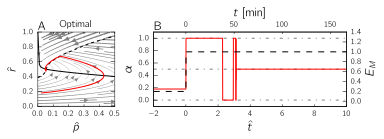
\includegraphics[clip,trim={0.4cm 0.5cm 0.54cm 0.45cm}]{./Fig/Fig4}
\caption{
\textbf{Optimal control of the self-replicator during a nutrient upshift.}
\textit{A:}~Optimal trajectory in the phase plane for the nondimensionalized model of Eqs~\ref{eq:pdefnondim}-\ref{eq:rdefnondim}, with streamlines. The optimal trajectory is shown as a solid, red curve.
The solid, black curve represents the $\hat{p}$-nullcline.
The dashed, black curve is the switching curve $\varphi(\hat{p})$.
The optimal solution was obtained by numerical optimization using \texttt{bocop}~\cite{bonnans_bocop_2012} (see \textit{Methods} for details), using the parameter values $E_M=1$ and $K=0.003$, and starting from the initial state $(0.024,0.18)$ at $t=0$ (optimal steady state for $E_M=0.2$).
\textit{B:}~Time evolution of the control variable $\alpha_{opt}(\cdot)$ (thick, red line) and the environment $E_M$ (dashed, black line).
}
\label{fig:optimalcontrol}
\end{figure}

In line with these results, we conjecture that the optimal solution consists in a switching transient towards the optimal steady state for the new environment, and remains at this steady state until the next environmental change.
Such a solution is known as a bang-bang-singular solution in the control theory literature~\cite{stengel_optimal_1994}.
Formally, the solution of Eq.~\ref{eq:J} can be described as
\begin{equation}
\label{eq:optcontrol}
\alpha_{opt}(\hat{t})=
\begin{cases}
0, \ \textrm{if} \ \hat{r}(\hat{t}) > \varphi(\hat{p}(\hat{t})),\\
1, \ \textrm{if} \ \hat{r}(\hat{t}) < \varphi(\hat{p}(\hat{t})), \\
\alpha^*_{opt}, \ \textrm{if} \ (\hat{p}(\hat{t}),\hat{r}(\hat{t}))=(\hat{p}_{opt}^*,\hat{r}_{opt}^*).
\end{cases}
\end{equation}
Notice that the optimal solution involves dynamical feedback from the state of the system to the control variable $\alpha(\cdot)$, and is therefore an instance of closed-loop optimization~\cite{stengel_optimal_1994}.

The optimal control problem of Eq.~\ref{eq:J} was also solved numerically by a direct method using the \texttt{bocop} software~\cite{bonnans_bocop_2012} (see \textit{Methods} for details).
A time discretization allows the problem to be transformed into a nonlinear optimization problem solved here by interior point techniques.
The optimal trajectories obtained numerically confirm our conjecture that the optimal control is bang-bang-singular.
An example solution, obtained by numerical optimization is shown in Fig.~\ref{fig:optimalcontrol}.
At time $\hat{t}=0$, $E_M$ jumps from a low to a high value, corresponding to a nutrient upshift (dashed black line in Fig.~\ref{fig:optimalcontrol}B).
The optimal solution $\alpha_{opt}$ consists of a sequence of switches between $\alpha=1$, corresponding to maximal synthesis of the gene expression machinery, and $\alpha=0$, corresponding to maximal synthesis of the metabolic machinery, until $(\hat{p}_{opt}^*,\hat{r}_{opt}^*)$ is reached.
$\alpha$ is then set to $\alpha^*_{opt}$, the value leading to the maximum growth rate in the new medium (here 0.5, for $E_M=1$).
The sequence of switches of $\alpha$ in Fig.~\ref{fig:optimalcontrol}\textit{B} corresponds to successive crossings of the switching curve in Fig.~\ref{fig:optimalcontrol}\textit{A}.
In particular, the switch just after $\hat{t}=2$ corresponds to the first crossing of the switching curve; the subsequent switches accumulate around the steady state and are therefore difficult to identify in the plot.

What is the biological relevance of the bang-bang-singular solution maximizing growth of the bacterial self-replicator?
In order to answer this question, we will investigate in the next two sections the different ways in which microorganisms could implement or have been shown to implement feedback growth control by sensing the environment and cellular physiology.
Although the idealized solution proposed by optimal control theory will obviously not be found in nature, actual control strategies may produce solutions that are close.
The optimal solution can thus be used as a gold standard, a benchmark for comparing actual control strategies. 

\subsection{Simple feedback control strategies: exploiting information on nutrients or precursors}
\label{sec:steadystate}

The control strategies that microbial cells have evolved to bring resource allocation in line with changes in the environment involve a variety of molecular mechanisms~\cite{chubukov_coordination_2014}.
These mechanisms are responsible for sensing the environment and the physiological state of the cell, as well as for adjusting the expression of genes that encode components of the transcriptional and translational machinery, enzymes, transporters, and proteins with other metabolic functions.

In the framework of the self-replicator model of bacterial growth, control strategies take the form of feedback control laws mapping the value of system variables to a value of the control variable $\alpha(\cdot)$.
In this section, we explore two such strategies, the first exploiting information on the quality and quantity of substrate present in the environment, as reflected in the value of $E_M$, and the second using information on the precursor concentration $\hat{p}$.
The feedback control strategies are graphically displayed in Fig.~\ref{fig:strategies_overview}, as an extension of the self-replicator of Fig.~\ref{fig:self_replicator}.
We pose a number of mathematical constraints on the feedback control strategies considered below.
First, we require the control laws to be functions of the variables of the self-replicator but not involve derivatives or integrals of these variables.
Second, for a constant environment $E_M$, the control strategies must drive the system to a unique stable and non-trivial steady state, enabling a non-zero growth rate.
Third, this steady state must equal the optimal steady state for that environment, given by $(\hat{p}_{opt}^*,\hat{r}_{opt}^*)$.


\begin{figure}[tb]
\centering
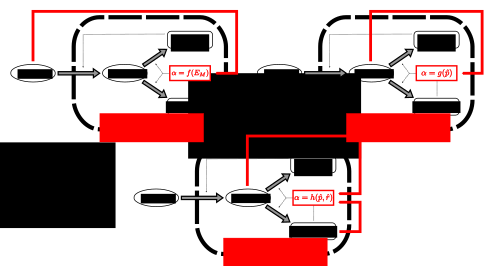
\includegraphics[width=\textwidth]{./Fig/Fig5}
\caption{
\textbf{Alternative strategies for controlling the self-replicator of bacterial growth.}
The feedback control strategies, shown in red and superposed on the self-replicator of Fig.~\ref{fig:self_replicator}, exploit information on system variables and the environment to adjust the value of $\alpha$, and thus the relative allocation of resources to the metabolic machinery and gene expression machinery.
}
\label{fig:strategies_overview}
\end{figure}


The first control strategy is defined by the function $f \colon \mathbb{R}^+ \to [0,1]$, mapping $E_M$ to $\alpha$:
\begin{equation}
\alpha = f(E_M).
\label{eq:f}
\end{equation}
Notice that $\alpha$ is constant because $E_M$ is fixed to the value defining the new environment after the upshift.
What would be an appropriate choice for $f$?
An advantage of the self-replicator model is that the optimal allocation at steady state can be explicitly formulated as a function of $E_M$ (Eq.~\ref{eq:alpha_mu_optimal} in \textit{Methods}, with derivation in \ref{S1_Text}).
This function is the unique function satisfying all of the above criteria (\ref{S1_Text}).
\ref{S1_Fig} plots $f$ and shows that it is conveniently approximated by a Michaelis-Menten function, \textit{i.e.},
\begin{equation}\label{eq:MMApprox}
\alpha(\cdot) = \dfrac{E_M}{E_M + K_{mE}},
\end{equation}
with the dimensionless half-saturation constant $K_{mE}$.
The interest of the approximation is that it demonstrates that the control strategy can be described by a simple and ubiquitous response curve in biochemical kinetics.
 
As an example of a regulatory system resembling the above control strategy consider the phosphotransferase system responsible for the uptake of glucose, the preferred substrate of \textit{E. coli}~\cite{deutscher_how_2006}.
In the presence of glucose, the EIIA\textsuperscript{Glc} component of the phosphotransferase system is mostly unphosphorylated, since the phosphate groups are used for the conversion of extracellular glucose to intracellular glucose-6-phosphate.
When glucose disappears from the medium, however, the glucose uptake rate decreases and, correspondingly, the phosphorylated fraction of EIIA\textsuperscript{\textrm{Glc}} increases.
The phosphorylation state of EIIA\textsuperscript{\textrm{Glc}} thus provides an indirect read-out of glucose availability.
In response to this signal, a variety of metabolic processes are upregulated or downregulated, notably involving the signalling molecule cAMP which activates the pleiotropic transcription factor Crp~\cite{deutscher_how_2006,gorke_carbon_2008}.

How does the control strategy of Eq.~\ref{eq:f}, which we call a nutrient-only strategy, perform in comparison with the optimal solution derived in the previous section?
That is, how much biomass does this strategy produce compared with the maximal amount of biomass that can theoretically be obtained after a nutrient upshift?
In order to answer these questions, we simulated the response to a sudden upshift of the self-replicator of Eqs~\ref{eq:pdefnondim}-\ref{eq:rdefnondim} controlled by the nutrient-only strategy of Eq.~\ref{eq:f}.
The results are shown in Fig.~\ref{fig:comparison_nutrients_precursor}.
Panel~\textit{A} shows the trajectory of the controlled self-replicator system and panel~\textit{D} plots the evolution of the amount of biomass as a fraction of the amount of biomass produced by the optimal strategy.
While the system does reach the steady state that is optimal for $E_M$, the nutrient-only strategy has poor performance in the transient phase immediately following the nutrient upshift.
As can be seen from the solution trajectory in Fig.~\ref{fig:comparison_nutrients_precursor}\textit{A}, fixing $\alpha$ to the value that enables optimal growth at steady state leads to a huge transient overshoot of the precursor concentration.
The overshoot reveals that resource allocation is initially suboptimal, with too many resources invested in the metabolic machinery at the expense of the gene expression machinery.
This causes a transiently suboptimal growth rate, leading to lower biomass accumulation (Eq.~\ref{eq:biomassdyn}).

\begin{figure}[p]
\centering
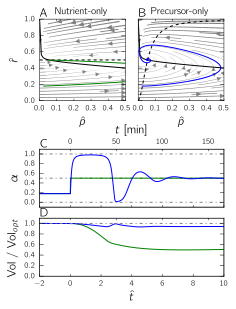
\includegraphics[scale=1]{./Fig/Fig6}
\caption{\small
\textbf{Comparison of the performance of the nutrient-only and precursor-only strategies after a nutrient upshift.}
\textit{A:}~Trajectory in the phase plane for the nutrient-only strategy (green curve).
The solid, black curve represents the $\hat{p}$-nullcline.
The dashed, black curve is the $\hat{r}$-nullcline.
The solution is obtained by numerical simulation of the system of Eqs~\ref{eq:pdefnondim}-\ref{eq:rdefnondim}, supplemented with $\alpha = f(E_M)$ as specified by Eq.~\ref{eq:meth_f} in the \textit{Methods} section and plotted in \ref{S1_Fig}.
The initial state corresponds to the steady state attained for an environment given by $0.2 \, E_M$.
While converging to the new steady state after the upshift, the precursor concentration makes a large overshoot.
\textit{B:}~As above, but for the precursor-only strategy.
The feedback control strategy is now defined by $\alpha = g(\hat{p})$ as specified by Eq.~\ref{eq:meth_g} in the \textit{Methods} section and plotted in \ref{S1_Fig}.
The solution trajectory (blue curve) exhibits a lower overshoot.
\textit{C:}~Evolution of the control variable $\alpha(\cdot)$ as a function of time, for each of the above two strategies.
Notice that in the nutrient-only strategy $\alpha(\cdot)$ immediately jumps to the optimal value for the post-upshift steady state (green curve), whereas in the precursor-only strategy it depends on the (time-varying) precursor concentration (blue curve).
\textit{D:}~Evolution of the ratio $\texttt{Vol} / \texttt{Vol}_{opt}$  as a function of time, where $\texttt{Vol}$ is the volume of the self-replicator and $\texttt{Vol}_{opt}$ the volume of the same replicator following the optimal strategy shown in Fig.~\ref{fig:optimalcontrol}.
In all of the above simulations, the parameter values $E_M=1$ and $K=0.003$ were used.
}
\label{fig:comparison_nutrients_precursor}
\end{figure}

One way to avoid the transient precursor imbalance observed in Fig.~\ref{fig:comparison_nutrients_precursor}\textit{A} would be to exploit information on the precursor concentration in the control strategy.
The second strategy considered here, which we label a precursor-only strategy, does exactly this: it involves a feedback control law $g \colon \mathbb{R}^+ \to [0,1]$ mapping $\hat{p}$ to $\alpha$:

\begin{equation}
\alpha = g(\hat{p}).
\label{eq:precursorstrategy}
\end{equation}
Since $\hat{p}$ will vary during the upshift experiment, $\alpha$ is not constant, contrary to the nutrient-only strategy above.
In the \textit{Methods} section, we present a function $g$ satisfying the requirements listed in the beginning of this section, in particular that the system converge to a stable steady state ensuring maximal growth in the new environment.
Moreover, we show that any other choice for $g$ leads to lower biomass production.
The function is plotted in \ref{S1_Fig}, and as shown in the same panel, is conveniently approximated by a Hill function with cooperativity coefficient 2:
\begin{equation}\label{eq:HillApprox}
\alpha (\cdot)= \dfrac{\hat{p}^2}{\hat{p}^2 + {K_{mp}}^2},
\end{equation}
where $K_{mp}$ is a dimensionless half-saturation constant.

While converging to the same steady state, this second strategy, which we will refer to as the precursor-only strategy, performs much better than the nutrient-only strategy after an upshift, as shown in Fig.~\ref{fig:comparison_nutrients_precursor}.
We simulated the response to a nutrient upshift of the self-replicator of Eqs~\ref{eq:pdefnondim}-\ref{eq:rdefnondim} with the precursor-only strategy of Eq.~\ref{eq:precursorstrategy}.
The relative biomass increases by 51\% and reaches 94\% of the biomass produced by the optimal control strategy (the theoretical maximum).
The precursor-only strategy notably avoids the inefficient transient accumulation of precursors directly after the nutrient upshift, by alternatingly investing more resources in gene expression (consumption of precursors) and metabolism (production of precursors).
In this respect, the oscillatory time profile of $\alpha$ (Fig.~\ref{fig:comparison_nutrients_precursor}\textit{C}) is somewhat reminiscent of the bang-bang-singular control in the solution of the optimal control problem (Fig.~\ref{fig:optimalcontrol}\textit{B}).

Both strategies, nutrient-only and precursor-only, drive the self-replicator towards the same steady state.
Whereas the two strategies are thus indistinguishable when the analysis is restricted to steady state, the precursor-only strategy is shown to perform much better in a dynamical upshift scenario, in the sense that the biomass produced is much closer to that produced by the optimal strategy.
Several authors have concluded that control strategies based on precursor sensing are key for maintaining optimal growth at steady state.
Scott \textit{et al.} argue that a strategy similar to the precursor-only approach above allows robust control of amino acid supply and demand, resulting in optimal steady-state growth over a range of nutrient conditions~\cite{scott_emergence_2014}.
They associate this strategy with ppGpp-mediated control of the synthesis of ribosomal proteins~\cite{dalebroux_ppgpp_2012,potrykus_pppgpp_2008,hauryliuk_recent_2015}.
The signalling molecule ppGpp accumulates in response to an increase in the level of uncharged tRNA, when amino acid concentrations in the cell drop. 
This causes ribosomes to "stall" and leads to RelA-mediated conversion of GTP to ppGpp, the molecular details of which are still subject of debate~\cite{english_singlemolecule_2011,hauryliuk_recent_2015}.
Since ppGpp inhibits the transcription of ribosomal RNAs~\cite{dennis_control_2004}, the concentration of the latter decreases, leading to more inactive ribosomal proteins and, through a well-characterized post-transcriptional autoregulatory mechanism, a lower synthesis rate of ribosomal proteins~\cite{keener_regulation_1996,potrykus_pppgpp_2008}.
Our analysis adds to the above study a novel insight: measuring precursors does not only enable resource allocation control to achieve maximal growth at steady state, but is also a good strategy in a dynamical context.

While the precursor-only strategy is thus seen to lead to good results, Fig.~\ref{fig:comparison_nutrients_precursor}\textit{D} shows that there remains room for improvement.
It seems reasonable to expect that control strategies exploiting information of not just a single variable, but several variables simultaneously, could further improve the performance of the self-replicator during a growth transition.


\subsection{A near-optimal feedback control strategy: exploiting information on the imbalance between precursors and the gene expression machinery}
\label{sec:strategies}

In the quest for further improvements, a natural starting-point would be to consider the curve defining the optimal steady states $(\hat{p}^*_{opt},\hat{r}^*_{opt})$  for different environments $E_M$.
This curve is defined by a function mapping $\hat{p}^*$ to $\hat{r}^*$, which is actually the same as the function $g$ introduced in the precursor-only strategy (\textit{Methods} and \ref{S1_Fig}), given that at steady state $\hat{r}=\alpha$ (Eq.~\ref{eq:rdefnondim}).
The curve can be seen as representing an optimal balance between precursors and the gene expression machinery, in the sense that the maximal growth rate attainable for a given precursor concentration $\hat{p}$ requires a concentration $\hat{r}$ of ribosomes and other components of the gene expression machinery equal to $g(\hat{p})$. 
If either $\hat{r}>g(\hat{p})$ or $\hat{r}<g(\hat{p})$, the growth rate is suboptimal.

These considerations suggest an intuitive control strategy, namely to avoid an imbalance between $\hat{p}$ and $\hat{r}$ at all times, and remain as close as possible to the curve defined by $g$.
In particular, when the gene expression machinery is more abundant than what is optimal given the available precursors ($\hat{r} > g(\hat{p})$), its synthesis is switched off ($\alpha = 0$).
Conversely, when $\hat{r} < g(\hat{p})$, synthesis of the gene expression machinery is switched on.
This strategy thus tries to restore "as quickly as possible" the optimal balance between precursors $\hat{p}$ and the gene expression machinery $\hat{r}$, giving rise to a so-called on-off control strategy:
\begin{equation}
\label{eq:stratswitch}
\alpha = h(\hat{p},\hat{r}) =
\begin{cases}
0, \ \textrm{if} \ \hat{r} > g(\hat{p}),\\
1, \ \textrm{if} \ \hat{r} < g(\hat{p}), \\
\alpha_{opt}^* \ \textrm{if} \ (\hat{p},\hat{r})=(\hat{p}_{opt}^*,\hat{r}_{opt}^*).
\end{cases}
\end{equation}

As shown in the \textit{Methods} section, the on-off strategy drives the system to a stable steady state ensuring growth at the maximal rate.
Notice that, contrary to the strategies discussed in the previous section, the value of $\alpha$ selected by the on-off strategy depends on both $\hat{p}$ and $\hat{r}$ (Fig.~\ref{fig:strategies_overview}).
It thus uses more information on the state of the system than the nutrient-only and precursor-only strategies.

Fig.~\ref{fig:onoffresults} shows the performance of the on-off strategy after a nutrient upshift, as compared to the precursor-only strategy.
The transition is seen to be nearly perfect, in the sense that 98\% of the optimal biomass is produced by the strategy.
The time course of $\alpha$ in panel \textit{D} is very similar to the optimal time course obtained by numerical optimization, shown in Fig.~\ref{fig:optimalcontrol}\textit{B}, and clearly brings out the bang-bang-singular nature of the solution. 
These results show that a strategy exploiting complete information on the internal state of the self-replicator can lead to near-optimal performance, outcompeting a strategy that uses partial information on the internal state (precursor abundance only).

\begin{figure}[p]
\centering
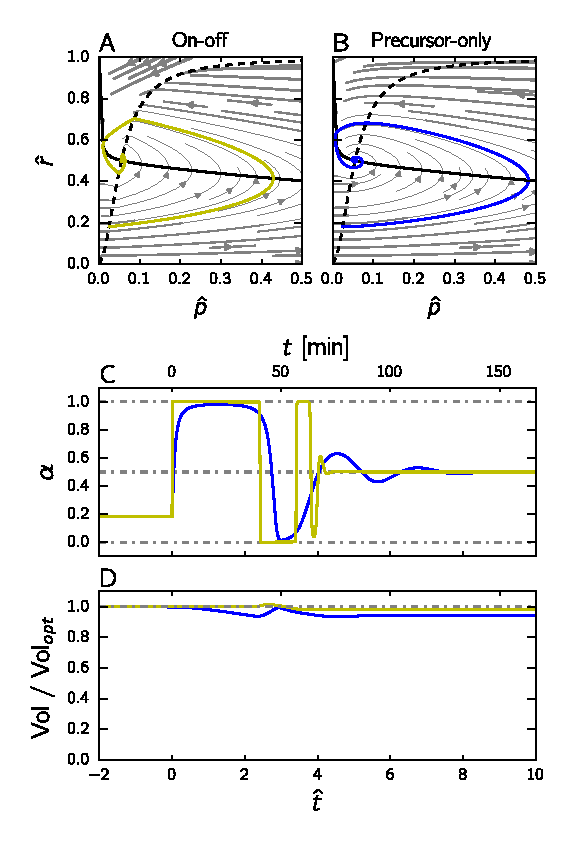
\includegraphics[scale=1]{./Fig/Fig7}
\caption{\small
\textbf{Comparison of the performance of the precursor-only and the on-off strategies after a nutrient upshift.}
\textit{A:}~Trajectory in the phase plane for the on-off strategy (yellow curve).
The solid, black curve represents the $\hat{p}$-nullcline and the dashed, black curve the function $g$.
The solution is obtained by numerical simulation of the system of Eqs~\ref{eq:pdefnondim}-\ref{eq:rdefnondim}, supplemented with the equation $\alpha = h(\hat{p},\hat{r})$ defined in Eq.~\ref{eq:stratswitch} and plotted in Fig.~\ref{fig:ppGppsurface}\textit{A}.
The initial state corresponds to the optimal steady state attained for an environment given by $0.2 \, E_M$.
\textit{B:}~Trajectory in the phase plane for the precursor-only strategy (same as in Fig.~\ref{fig:comparison_nutrients_precursor}\textit{B}, added for comparison).
\textit{C:}~Evolution of the control variable $\alpha$ for each strategy as a function of time.
Both strategies stabilize the system at the optimal steady state, but only the on-off strategy (yellow curve) exhibits bang-bang behavior.
\textit{D:}~Evolution of the ratio $\texttt{Vol} / \texttt{Vol}_{opt}$ for the on-off and precursor-only strategies as a function of time, where $\texttt{Vol}$ is the volume of the self-replicator and $\texttt{Vol}_{opt}$ the volume of the same replicator following the optimal strategy shown in Fig.~\ref{fig:optimalcontrol}.
The final values of $\texttt{Vol} / \texttt{Vol}_{opt}$ attained by the two strategies are 0.9831 and 0.9413, respectively.
The on-off strategy is thus hardly distinguishable from the optimal control strategy in the plot.
In all of the above simulations, the parameter values $E_M=1$ and $K=0.003$ were used.
}
\label{fig:onoffresults}
\end{figure}

Are microbial cells equipped with mechanisms implementing a strategy similar to the on-off strategy?
A possible candidate would again be the ppGpp system.
A kinetic model of ppGpp metabolism and the regulation of the synthesis of ribosomal proteins was recently presented by Bosdriesz \textit{et al.}~\cite{bosdriesz_how_2015}.
The model proved capable of accounting for a range of experimental data, including the steady-state concentration of ppGpp as a function of the growth rate~\cite{bremer_modulation_1996} and the dynamical response of ppGpp to a nutrient upshift or downshift~\cite{murray_control_2003}.
A major conclusion of the model is that the steady-state concentration of ppGpp exhibits a strongly ultrasensitive response to deviations of the ribosomal protein fraction from the optimal ribosomal protein fraction at a given growth rate. 
These deviations from optimality, in turn, lead to a switch-like response of the synthesis rate of ribosomal proteins (Fig.~4 in Bosdriesz \textit{et al.}~\cite{bosdriesz_how_2015}).

How does this mechanistic model of ppGpp regulation relate to the on-off strategy presented above?
In order to answer this question, we first need to find a correspondence between the variables $p$ and $r$ of our coarse-grained model and the concentrations of molecular species in the kinetic model of Bosdriesz \textit{et al.}
This is rather straightforward to achieve, by equating $p$ to the total amino acid concentration and $r$ to the ribosome concentration.
Second, \ref{S4_Text} shows that by making two simplifying assumptions, ppGpp can be expressed as a function of the total amino acid concentration and the ribosome concentration.
In particular, we assume that concentrations of all individual amino acids are equal, and that the concentrations of charged tRNAs and ppGpp evolve fast relative to the dynamics of the amino acid and ribosome concentrations.
The third step consists in positing an explicit relation between ppGpp and $\alpha$, based on the regulatory action of ppGpp on the transcription of ribosomal RNA~\cite{dennis_control_2004}:

\begin{equation}
\alpha(\cdot) = \frac{K_I}{K_I + \texttt{ppGpp}(\cdot)},
\label{eq:ppGpp_empirical}
\end{equation}
with $K_I$ a Michaelis-Menten inhibition constant [$\mu$mol~L\textsuperscript{-1}] and $\texttt{ppGpp}$ the (time-varying) intracellular concentration of ppGpp [$\mu$mol~L\textsuperscript{-1}].

The response function for ppGpp thus obtained and evaluated for a range of amino acid and ribosome concentrations is represented in Fig.~\ref{fig:ppGppsurface}, and visually compared with the on-off strategy.
As can be seen, the two response surfaces are very similar.
In other words, the ultrasensitive response of the synthesis rate of ribosomal proteins to the suboptimal allocation of cellular resources, derived from a model of the molecular mechanisms involved in the synthesis, degradation, and regulatory action of ppGpp~\cite{bosdriesz_how_2015}, implements a control strategy that is close to the optimal predicted by a control-theoretical analysis of the self-replicator.
While the role of ppGpp in maintaining optimal resource allocation was already pointed out by Scott \textit{et al.} and Bosdriesz \textit{et al.}, the latter studies were restricted to optimizing steady-state growth.
A major insight from the analysis in this section is that this conclusion seems to carry over to dynamical scenarios as well.
Fundamentally, the analysis suggests that the ppGpp system is a likely candidate to fulfill this role because it integrates information on the imbalance between precursor concentration and abundance of the gene expression machinery.

\begin{figure}[tb]
\centering
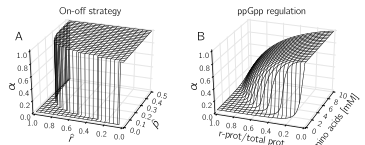
\includegraphics[scale=1]{./Fig/Fig8}
\caption{
\textbf{ppGpp regulation implements an on-off control strategy of resource allocation.}
\textit{A:}~Response surface of the on-off control strategy, defined by $\alpha = h(\hat{p},\hat{r})$ in Eq.~\ref{eq:stratswitch}.
\textit{B:}~Response surface of the ppGpp control strategy, as defined by Eq.~\ref{eq:ppGpp_empirical} and the simplified kinetic model defining ppGpp in terms of the total amino acid concentration and the ribosomal protein fraction (\ref{S4_Text}).
The shape of the response surface of the ppGpp control strategy is seen to be in very good agreement with the on-off strategy leading to near-optimal performance of the self-replicator during a nutrient upshift.
}
\label{fig:ppGppsurface}
\end{figure}

\section{Discussion}
\label{sec:discussion}

Quantitative growth laws are empirical regularities pointing at fundamental properties of microbial life~\cite{scott_bacterial_2011}.
Recent work has led to the precise theoretical formulation of growth laws and has shown that they can be derived from basic assumptions on the molecular processes responsible for the assimilation of nutrients and their conversion to biomass~\cite{bosdriesz_how_2015,maitra_bacterial_2014,molenaar_shifts_2009,scott_emergence_2014,weisse_mechanistic_2015}.
The growth laws are uniquely defined under the hypothesis that microorganisms allocate resources in such a way as to maximize their growth rate.
Several of the above-mentioned studies have analyzed feedback control strategies on the molecular level enabling cells to achieve optimal resource allocation in a robust manner.
The control strategies exploit information on the physiological state of the cell to adjust the (relative) rate of synthesis of different classes of proteins (ribsomes, metabolic enzymes, $\ldots$).
Whereas the growth laws describe microbial growth at steady state, most microorganisms live in complex, continuously changing environments.
Despite some precursory work~\cite{pavlov_optimal_2013,vandenberg_optimal_1998}, questions about the dynamics of microbial growth remain largely unanswered:
Which resource allocation schemes are optimal in changing environments? Which dynamical control strategies lead to (near-)optimal resource allocation? How do these strategies compare with those actually implemented by microorganisms? 

We have addressed the above questions by means of a self-replicator model of microbial growth, which, like other coarse-grained models of bacterial growth~\cite{maitra_bacterial_2014,molenaar_shifts_2009,scott_emergence_2014}, is capable of reproducing the growth laws at steady state (Fig.~\ref{fig:model_validation}).
A first major contribution of our work is to show that, in the case of a dynamical upshift scenario, optimal production of biomass requires a bang-bang-singular resource allocation scheme (Fig.~\ref{fig:optimalcontrol}).
That is, the optimal self-replicator should iteratively allocate all of its resources to the gene expression machinery (bang control input) and the metabolic machinery (another bang control input), until the steady state enabling maximal growth in the post-upshift environment is reached, corresponding to a trade-off in the allocation of resources to the two processes (singular control input).

Bang-bang phenomena are widespread in a variety of life processes.
Applications of optimal control theory to reproductive strategies in insects~\cite{macevicz_modeling_1976}, the development of intestinal crypts~\cite{itzkovitz_optimality_2012}, and the activation of metabolic pathways~\cite{bartl_modelling_2010,oyarzun_sequential_2009} have led to bang-bang or bang-bang-singular strategies.
In optimal control problems, such a solution arises with systems where the differential equations are linear in the control variable (in our case, $\alpha (\cdot)$).
Examples of applications that are close to the problem considered here are the control of gene expression for adaptation to environmental changes~\cite{pavlov_optimal_2013, madar_promoter_2013}, and the allocation of resources between nutrient uptake and growth in microorganisms~\cite{vandenberg_optimal_1998, kiselev_resource_2009}.
Whereas the former applications focus on minimization of response times, the latter also optimize biomass during a growth transition, using a different model, not derived from first principles as in this study.
However, the optimal solution of the corresponding optimal control problem is also bang-bang-singular, thus showing that our conclusions are robust to model variations.

Our second major contribution is the assessment of how different feedback control strategies perform with respect to each other and to the gold standard determined from optimal control theory.
We show that the precursor-only and nutrient-only strategies, both of which drive the self-replicator to the steady state with maximal growth rate in a static environment, perform quite differently in a dynamical upshift scenario (Fig.~\ref{fig:comparison_nutrients_precursor}).
While the precursor-only strategy is better than the nutrient-only strategy in a dynamical environment, it is in turn outperformed by a so-called on-off strategy, which achieves a near-perfect growth transition by exploiting information on the imbalance between the precursor concentration and the abundance of the gene expression machinery (Fig.~\ref{fig:onoffresults}).
The superior performance of the on-off strategy can be intuitively explained by the fact that during a growth transition the two variables are not fully correlated, which means that sensing both instead of either one provides additional information in a dynamical context.

Interestingly, the on-off strategy is based on a feedback control law that very much resembles the response function for ppGpp-mediated regulation of the synthesis of ribosomal RNAs in \textit{E. coli}~\cite{bosdriesz_how_2015}.
The role of ppGpp in controlling microbial growth has been amply documented~\cite{dalebroux_ppgpp_2012,potrykus_pppgpp_2008,hauryliuk_recent_2015}.
For example, Potrykus \textit{et al.} observed that in cells without ppGpp (ppGpp$^0$ mutants) the RNA/protein mass ratio, a proxy for our resource allocation variable $\alpha$, does not change with the growth rate, which has led these authors to conclude that ppGpp is the major source of growth-rate control in \textit{E. coli}~\cite{potrykus_ppgpp_2011}.
The central importance of ppGpp in the reallocation of gene expression resources in \textit{E. coli} following changes in nutrient availability has also been mapped with higher resolution, using genome-wide transcriptome studies~\cite{traxler_guanosine_2006,traxler_global_2008}.
In nearly all bacterial species examined so far, ppGpp is known to accumulate in response to an increase in the level of uncharged tRNA~\cite{gaca_many_2015}, although the molecular details of ppGpp metabolism and the range of other functions of the alarmone may greatly vary across species~\cite{gaca_many_2015,hauryliuk_recent_2015,liu_diversity_2015}.
While it has thus been well-established that regulation by ppGpp is an evolutionary conserved mechanism of growth control in the bacterial cell, our analysis provides a new perspective by suggesting that ppGpp enables optimal reallocation of resources after a growth transition, dynamically maximizing the accumulation of biomass.

The model on which the above results are based is built from first principles by distinguishing two fundamental cellular processes: metabolism (converting nutrients to precursors) and gene expression (converting precursors to the proteins that make up biomass) (Fig.~\ref{fig:self_replicator}). 
Despite its simplicity, our self-replicator model is capable of reproducing the empirical growth laws and of making testable predictions on the time-course profile of the resource allocation variable $\alpha$ and on the concentrations $p$ and $r$ of components of the gene expression machinery and metabolic machinery, respectively (see Fig.~\ref{fig:ppGppsurface} and below). 
The model can be easily extended with more details on protein synthesis, central carbon and energy metabolism, stress systems, or cell membranes, but this would make the mathematical analysis of the model dynamics and the optimal control problem more complicated. 
Notice, however, that the direct numerical approach for solving the optimal control problem remains applicable, even for more fine-grained models (Fig.~\ref{fig:optimalcontrol}, see also~\cite{waldherr_dynamic_2015}).

The comparison of different control strategies during a classical growth transition should be interpreted carefully, in a qualitative rather than quantitative manner. 
Whereas the differences in performance based on the biomass ratio $\texttt{Vol} / \texttt{Vol}_{opt}$ of the control strategies are robust, the absolute numbers for the biomass ratio will depend on details of the growth experiment chosen and the exact parameter values. 
Another implicit assumption in the analysis of the control strategies is that the costs of their molecular implementation can be neglected.
This is not true in general, since every control strategy requires resources to be diverted towards the synthesis of sensory systems and regulatory proteins, with possibly detrimental effects on growth.
In other words, a control strategy entails a trade-off between the growth burden of regulation and the growth benefit of the improved capability to adapt to changes in the environment~\cite{kalisky_costbenefit_2007,poelwijk_tradeoffs_2011}. 
The analysis of control strategies could be refined by adding a reaction to the self-replicator that models the loss of resources incurred by regulatory strategies.
While in general the growth burden of a control strategy requiring information on several aspects of cellular physiology is expected to be higher, notice that a single regulatory system may be capable of sensing more than one variable.
For example, we show that ppGpp levels in the cell carry information on both the metabolic and the gene expression state (Fig.~\ref{fig:ppGppsurface}), thus integrating several signals in a cost-efficient manner. 

The model predictions for the dynamical adaptation of resource allocation after a nutrient upshift suggest several interesting experimental tests.
In particular, the switching profile of the resource allocation variable $\alpha$ is a promising candidate for experimental validation. 
The most straightforward option would be direct measurement of the synthesis rate of ribosomal proteins, using a translational fusion of a fluorescent reporter with a ribosomal protein~\cite{bakshi_superresolution_2012,english_singlemolecule_2011}.
However, a more indirect approach based on the quantification of ppGpp concentrations in the cell or the activity of the ribosomal RNA (rRNA) promoters would also be a possibility.
Interestingly, some data are already available in the literature.
For instance, Gausing has reviewed data on the synthesis of ribosomal proteins after a nutrient upshift, showing that the synthesis rate goes through "a series of rapid changes" resembling oscillations~\cite{gausing_regulation_1980}.
Later work attributed this pattern to regulation on the transcriptional level~\cite{zengel_transcription_1986}.
Friesen \textit{et al.} observed oscillatory patterns in ppGpp concentrations after a nutrient upshift, with an initial response resembling bang control for an upshift to a particularly rich medium~\cite{friesen_synthesis_1975}.
Murray \textit{et al.} also present data on the ppGpp concentration after a nutrient upshift~\cite{murray_control_2003}, but with a lower temporal resolution and no clear oscillatory pattern.
All of the above measurements were carried out on the population level, which means that switching patterns may be obscured by desynchronisation of the individual cells.
More sophisticated experimental set-ups are necessary for the decisive validation of the model predictions, allowing gene expression in single cells to be followed over time in tightly regulated growth conditions~\cite{young_measuring_2011,duncombe_microfluidics_2015}.
In addition, the model could be validated on other dynamical scenarios, for example nutrient downshifts~\cite{molin_control_1977,murray_control_2003}.

Apart from its interest for fundamental science, resource allocation is also a critical question in biotechnology, where there exists an inherent trade-off between the maximization of yield and productivity\cite{venayak_engineering_2015}.
High yield means that most of the substrate is converted to a metabolite, peptide or recombinant protein of interest, but this leads to low productivity if the remaining nutrient influx is insufficient to sustain population growth.
Engineered control of resource allocation may help in establishing the right trade-off, the most profitable balance between yield and productivity, in a biotechnological process.
Such a trade-off could be attained either in steady-state conditions (the incoming nutrient flux is optimally distributed over growth and production) or in dynamical conditions (alternating utilization of the incoming nutrient flux for growth or production)~\cite{dahl_engineering_2013,xu_improving_2014,izard_synthetic_2015}.
When extended with heterologous metabolic pathways, the self-replicator models used in this study would provide an adequate \textit{in-silico} test bed for the rapid screening and comparison of alternative control strategies in bioprocess engineering.
 
%%%%%%%%%%%%%%%%%%%%%%%%%%%%%%%%

\section{Methods}

\subsection{Steady-state analysis of model}
\label{sec:methods_model_analysis}

The nondimensional version of the model, given by Eqs~\ref{eq:pdefnondim}-\ref{eq:rdefnondim}, was used for a steady-state analysis of the self-replicator.
Eqs~\ref{eq:pdefnondim}-\ref{eq:rdefnondim} were derived from the original model of Eqs~\ref{eq:pdef}-\ref{eq:rdef} by means of the following rescalings:
\begin{equation*}
\hat{p}  = \beta \, p,\;\;\;
\hat{r}  = \beta \, r,\;\;\;
\hat{t}  = k_R \, t,\;\;\;
E_M = e_M/k_R,\;\;\;
K = \beta K_R.
\end{equation*}

As shown in \ref{S1_Text}, for a constant environment $E_M$ and constant resource allocation $\alpha$, the system has two steady states: a trivial unstable steady state $(\hat{p}^*, \hat{r}^*) = (0,1)$, allowing no growth in the absence of precursors, and a steady state with a positive growth rate given by
\begin{equation}
\label{eq:meth_steadystate}
(\hat{p}^*, \hat{r}^*) = \left( \frac{(1-\alpha)\, E_M - \alpha + \sqrt{[(1-\alpha)\, E_M - \alpha]^2 + 4\alpha\, (1-\alpha)\, E_M\, K}}{2\alpha}, \alpha \right).
\end{equation}
The two eigenvalues of the Jacobian matrix evaluated at $(\hat{p}^*, \hat{r}^*)$ are negative (\ref{S1_Text}), so that this steady state is stable.

The growth rate at steady state, as a function of $\hat{p}^*$ and $\hat{r}^*$, is given by Eq.~\ref{eq:munondim}, which we repeat here for clarity:
\begin{equation*}
\hat{\mu}^* = \frac{\hat{p}^*}{K + \hat{p}^*} \, \hat{r}^* .
\end{equation*}
Evaluating $d\hat{p}/dt=0$ at $(\hat{p}^*, \hat{r}^*)$ allows $\hat{r}^*$, and therefore $\hat{\mu}^*$, to be written as a function of $\hat{p}^*$ (\ref{S1_Text}).
Accordingly, we can compute $\partial\hat{\mu}^*/\partial\hat{p}^*$ and, when setting this partial derivative to 0, determine the maximum growth rate at steady state $\mu_{opt}^*$ and the optimal resource allocation $\alpha_{opt}^*$ bringing about this maximal growth rate.
As shown in \ref{S1_Text}, $\mu_{opt}^*$ and $\alpha_{opt}^*$ can be written as explicit functions of either the environment $E_M$:
\begin{equation}
\label{eq:alpha_mu_optimal}
\alpha_{opt}^* = \frac{E_M + \sqrt{K\, E_M}}{E_M + 2\sqrt{K\, E_M} + 1}
, \;\;\;\;\;\;\;\;\;\;\;\;\;\; 
\hat{\mu}^*_{opt} = \frac{E_M}{E_M + 2\sqrt{K\, E_M} + 1},
\end{equation}
or the precursor abundance $\hat{p}_{opt}^*$:
\begin{equation}
\label{eq:alpha_mu_optimal_p}
\alpha_{opt}^* = \frac{\hat{p}^{*}_{opt}}{\hat{p}^{*}_{opt} + \frac{K}{K+\hat{p}^{*}_{opt}}(1+\hat{p}^{*}_{opt})}
, \;\;\;\;\;\;\;\;\;\;\;\;\;\; 
\hat{\mu}^*_{opt} = \frac{\hat{p}^{* 2}_{opt}}{\hat{p}^{* 2}_{opt} + 2K\hat{p}^*_{opt} + K}.
\end{equation}
The above equations were used for the derivation of the control strategies (see below).


\subsection{Model fitting}
\label{sec:methods_model_fitting}

As can be seen by comparing Figs~\ref{fig:model_validation}\textit{A} and~\ref{fig:model_validation}\textit{B}, growth-rate maximization in the self-replicator model leads to a good qualitative correspondence with the growth laws.
In order to determine if a good quantitative fit of the model with the data from Scott~\textit{et al.} \cite{scott_interdependence_2010} can be obtained, for reasonable parameter values, we estimated $e_M$ and $k_R$ in Eqs~\ref{eq:pdef}-\ref{eq:rdef} from the measured RNA/protein mass ratios.
At steady state, the RNA/protein mass ratio can be interpreted as proportional to $\hat{r}^*$ (and thus $\alpha_{opt}^*$), with an unknown (dimensionless) proportionality constant $\gamma$ (see~\cite{scott_interdependence_2010} for details on the use of the RNA/protein mass ratio as a proxy for the ribosomal protein mass fraction):
\begin{equation}
\hat{r}^* = \alpha_{opt}^* = \gamma \, \frac{\text{RNA mass}}{\text{protein mass}}.
\label{eq:gamma}
\end{equation}
Reformulating Eq.~\ref{eq:alpha_mu_optimal} in terms of the original parameters $e_M$ and $k_R$, which have physical dimensions facilitating the biological interpretation of their values, we obtain a straighforward relation between $e_M$, $k_R$, $K$, $\alpha_{opt}^*$ and $\mu_{opt}^*$:
\begin{equation}
\label{eq:alpha_mu_optimal_dim}
\alpha_{opt}^* = \frac{e_M + \sqrt{K\, e_M\, k_R}}{e_M + 2\sqrt{K\, e_M\, k_R} + k_R}
, \;\;\;\;\;\;\;\;\;\;\;\;\;\; 
\mu^*_{opt} = \frac{e_M \, k_R}{e_M + 2\sqrt{K\, e_M\, k_R} + k_R}.
\end{equation}

Eqs~\ref{eq:gamma}-\ref{eq:alpha_mu_optimal_dim} were used to estimate values of $k_R$ and $\gamma$, as well as $e_M$ for each of the six growth conditions, from the measurements of the growth rate and the RNA/protein mass ratio. 
The value $K$ was not estimated from the experimental data, but set to a value inferred from the literature (\ref{S1_Text}).
The optimization process was carried out by means of the differential evolution algorithm of Storn and Price~\cite{storn_differential_1997}.
The results are shown in Fig.~\ref{fig:model_validation}\textit{B}, while the estimated parameter values are summarized in \ref{S1_Table}.
The parameter values are in very good agreement with order-of-magnitude values determined from the literature (\ref{S2_Text} and \ref{S1_Table}). 

\subsection{Solution of optimal control problem}

The optimal control problem of Eq.~\ref{eq:J} consists in identifying the function $\alpha_{opt}(t)$ that maximizes the integral of the growth rate $\hat{\mu}$ over an interval $[0, \tau]$.
In order to solve this problem, we first redefined it over an infinite horizon (\textit{i.e.}, $\tau \rightarrow \infty $) in order to avoid boundary effects occurring over finite time intervals, in particular the depletion of precursors just before reaching $\tau$.
With $\mathcal{U}=\{\alpha:\mathbb{R}^+ \rightarrow [0,1] \}$ the set of admissible controls, the full optimization problem for the nondimensionalized system is given by
\begin{equation}\label{eq:meth_prob}
\max_{\alpha \in \mathcal{U}} J(\alpha)\equiv \int_0^{\infty} \hat{r}(\hat{t}) \, \dfrac{\hat{p}(\hat{t})}{K+\hat{p}(\hat{t})}\, d\hat{t}.
\end{equation}
Since $J(\alpha)$ diverges, we actually consider overtaking optimality:
A solution is overtaking optimal if its performance index catches up with the performance index of any other solution (\cite{carlson_infinite_1991}, see \ref{S3_Text} for details).

Necessary conditions on optimal trajectories can be obtained by the Infinite Horizon Maximum Principle \cite{carlson_infinite_1991}, an extension of the well-known Pontryagin Maximum Principle.
Analysis of the Hamiltonian of the system of Eqs~\ref{eq:pdefnondim}-\ref{eq:rdefnondim} and the associated adjoint system shows that the optimal trajectory is a concatenation of bang arcs ($\alpha(\cdot)=0$ or $\alpha(\cdot)=1$) and possibly a singular arc corresponding to the optimal steady state $(\hat{p}(t),\hat{r}(t))=(\hat{p}_{opt}^*,\hat{r}_{opt}^*)$, that is, the steady state leading to the optimal growth rate $\hat{\mu}_{opt}^*$ in the new environment after the upshift (\ref{S3_Text}).
Moreover, from the Kelley condition~\cite{borisov_fullers_2000}, we can show that if the optimal trajectory has a singular arc, then it must enter this singular arc \textit{via} a chattering arc, \textit{i.e.}, with an infinite number of switches of $\alpha (\cdot)$ between 0 and 1 (\ref{S3_Text}).
The chattering arc is characterized by a switching curve $\hat{r}=\varphi(\hat{p})$ in the $(\hat{p},\hat{r})$-plane, which passes through $(\hat{p}_{opt}^*,\hat{r}_{opt}^*)$.
The switching curve divides the phase plane into two regions, such that $\alpha(t)$ switches to 0 when the system is in the region above $\varphi$ and to 1 when the system is below $\varphi$ (\ref{S3_Text} and Fig.~\ref{fig:optimalcontrol}).

The above results have led to the conjectured optimal solution of Eq.~\ref{eq:optcontrol}.
In parallel, we numerically solved the problem of Eq.~\ref{eq:meth_prob} by a direct method using the \texttt{bocop} software~\cite{bonnans_bocop_2012}.
A time discretization allows the optimal control problem to be transformed into a nonlinear optimization problem,
solved here by interior point techniques.
A discretization by a Lobatto IIIC formula (6th order) was used with 4000 time steps, and the relative tolerance for the NLP solver was set to $10^{-14}$.
The optimal trajectories thus obtained are composed of a chattering arc followed by a steady state corresponding to the singular arc (Fig.~\ref{fig:optimalcontrol}).
The switching curve $\varphi(\hat{p})$ was computed from numerical simulations with different initial conditions. 

\subsection{Specification and analysis of control strategies}

As described in the \textit{Results} section, we are interested in control strategies satisfying the following conditions:
\begin{description}
\item[(C1)] The control laws are static functions of the system variables (as opposed to, for instance, functions that depend on derivatives or integrals of the variables).
\item[(C2)] For any given constant environment $E_M$, they drive the self-replicator system towards a unique stable steady state that is not trivial, \textit{i.e.}, with nonzero growth rate.
\item[(C3)] This steady state corresponds to the optimal steady state $(\hat{p}_{opt}^*, \hat{r}_{opt}^*)$, allowing growth at the maximal rate $\mu^*_{opt}$.
\end{description}
It can be directly verified from the functions $f$, $g$, and $h$ defining the nutrient-only, precursor-only, and on-off control strategies (Eqs~\ref{eq:f}, \ref{eq:precursorstrategy}, and \ref{eq:stratswitch}) that they are indeed static functions of the system variables (or the system input, in the case of the nutrient-only strategy). 
Here we show that the other two conditions are also satisfied for all three strategies.

Following Eq.~\ref{eq:f}, the nutrient-only strategy is defined by $\alpha = f(E_M)$, so that $\alpha$ is constant after the upshift.
As shown above and in \ref{S1_Text}, this means that the system controlled by the nutrient-only strategy has a single nontrivial stable steady state (Condition~C2). 
In addition, in this case the optimal steady state is attained for $\alpha^*_{opt}$ defined as in Eq.~\ref{eq:alpha_mu_optimal}, and the following function $f$ therefore guarantees Condition~C3:
\begin{equation}
\label{eq:meth_f}
f(E_M) = \frac{E_M + \sqrt{K E_M}}{E_M + 2\sqrt{K\, E_M} + 1}.
\end{equation}
In \ref{S1_Text}, it is shown that Eq.~\ref{eq:meth_f} is the only definition of $f$ satisfying all conditions.
\ref{S1_Fig} shows a plot of $f(E_M)$ together with a biologically plausible Michaelis-Menten approximation (Eq.~\ref{eq:MMApprox}).

The full specification of the precursor-only strategy demands an expression for the function $g$ in Eq.~\ref{eq:precursorstrategy}.
Recall that Eq.~\ref{eq:alpha_mu_optimal_p} defines $\alpha_{opt}^*$ in terms of the precursor concentration $\hat{p}_{opt}^*$, which leads us to propose the following function $g$:
\begin{equation}
\label{eq:meth_g}
g(\hat{p}) = \frac{\hat{p}}{\hat{p} + \frac{K}{K + \hat{p}}(1+\hat{p})}.
\end{equation}
As shown in \ref{S1_Text} by computing the Jacobian, the system given by Eqs~\ref{eq:pdefnondim}-\ref{eq:rdefnondim} and \ref{eq:meth_g} has a single nontrivial stable steady state for any environment $E_M$ (Condition~C2).
Moreover, Eq.~\ref{eq:meth_g} guarantees this steady state to be optimal (Condition~C3).
This can be seen by noting that at steady state, $d\hat{r}/dt=0$ implies $\hat{r}^*=g(\hat{p}^*)$ (Eq.~\ref{eq:rdefnondim}).
In order for the self-replicator to attain a maximal growth rate at steady rate, Eq.~\ref{eq:alpha_mu_optimal_p} needs to be satified, which is the case for the above choice of the function $g$.
Like for $f$, Eq.~\ref{eq:meth_g} is the only choice for $g$ satisfying C1-C3.
\ref{S1_Fig} shows a plot of $g(\hat{p})$ together with a biologically plausible Hill approximation (Eq.~\ref{eq:HillApprox}).

The on-off control strategy is defined in Eq.~\ref{eq:stratswitch} and repeated below:
\begin{equation}
h(\hat{p}, \hat{r}) = 
\begin{cases}
0, \ \textrm{if} \ \hat{r} > g(\hat{p}),\\
1, \ \textrm{if} \ \hat{r} < g(\hat{p}), \\
\alpha_{opt}^*, \ \textrm{if} \ (\hat{p},\hat{r})=(\hat{p}_{opt}^*,\hat{r}_{opt}^*).
\end{cases}
\end{equation}
This strategy drives the system to a single steady state, because the $\hat{p}$-nullcline crosses the function $g(\hat{p})$ only once, as shown graphically in Fig.~\ref{fig:onoffresults}\textit{A}.
In \ref{S1_Text} we argue that this steady state is stable, by taking into account so-called sliding modes on the switching curve~\cite{filippov_differential_1988} (Condition~C2).
Moreover, the steady state coincides with the optimal steady state $(\hat{p}_{opt}^*,\hat{r}_{opt}^*)$ by construction, so that Condition~C3 is satisfied as well.
Fig~\ref{fig:ppGppsurface}\textit{A} shows a plot of $h(\hat{p}, \hat{r})$.

Note that since $h(\cdot)$ is discontinuous, numerical instabilities occur during simulations.
We therefore used the following continuous approximation of this function:
\begin{equation}
\frac{g(\hat{p})^{100}}{g(\hat{p})^{100} + \hat{r}^{100}}, \ \textrm{if} \ \hat{r} \neq g(\hat{p}).
\end{equation}
The approximation causes $\alpha$ to take intermediate values (instead of 0 or 1) just before reaching the optimal steady state in Fig~\ref{fig:onoffresults}\textit{C}.
For numerical simulations of the ODE system, we used the CVODE solver~\cite{cohen_cvode_1996} from SUNDIALS 2.6.2~\cite{hindmarsh_sundials_2005}.

\clearpage

\section{Supporting information for Chapter~2}

\subsection{S1 Text -- Model derivation and analysis}
\manuallabel{S1_Text}{S1~Text}

\subsubsection{Model formulation}

The time evolution of the total mass of each component of the self-replicator can be written as follows:
\begin{eqnarray}
\frac{dP}{dt} &=& V_M(t) - V_R(t) \nonumber , \\
\frac{dM}{dt} &=& (1-\alpha(t))\, V_R(t) \label{eq:ext_system},\\
\frac{dR}{dt} &=& \alpha(t) \, V_R(t)  \nonumber ,
\end{eqnarray}
where $P$, $M$, $R$ [g] denote the total mass of precursors, metabolic machinery and gene expression machinery, respectively.
$V_M$ [g h$^{-1}$] is the rate of production of precursors by metabolism and $V_R$ [g h$^{-1}$] the rate of utilisation of precursors for gene expression.

Dividing the mass variables by the total time-varying volume $\texttt{Vol}(t)$ of the system, we obtain the concentration variables $p = P/\texttt{Vol}$, $m = M/\texttt{Vol}$, $r = R/\texttt{Vol}$ [g L$^{-1}$].
The dynamics of the concentration variables then follows with Eq.~\ref{eq:ext_system}:
\begin{eqnarray}
\frac{dp}{dt} &=& \frac{V_M(t)}{\texttt{Vol}} - \frac{V_R(t)}{\texttt{Vol}} - \frac{1}{\texttt{Vol}}\frac{d\texttt{Vol}}{dt}\, p, \nonumber \\
\frac{dm}{dt} &=& (1-\alpha(t)) \frac{V_R(t)}{\texttt{Vol}} - \frac{1}{\texttt{Vol}}\frac{d\texttt{Vol}}{dt} \, m  \label{eq:deriv_int_system},\\ 
\frac{dr}{dt} &=& \alpha(t) \, \frac{V_R(t)}{\texttt{Vol}}  - \frac{1}{\texttt{Vol}}\frac{d\texttt{Vol}}{dt} \, r. \nonumber
\end{eqnarray}

At this point, we define $v_M = V_M/\texttt{Vol}$ and $v_R = V_R/\texttt{Vol}$ [g L$^{-1}$ h$^{-1}$] as the mass fluxes per unit volume.
Moreover, with the definition of the volume in terms of the total protein mass in Eq.~\ref{eq:voldef} of the main text, that is, $\texttt{Vol} = \beta\, (M + R)$, we find that
\begin{equation}
\label{eq:supp_deriv_growthrate}
\frac{1}{\texttt{Vol}} \frac{d\texttt{Vol}}{dt} = \frac{\beta}{\texttt{Vol}} \frac{d(M+R)}{dt} = \beta\, \frac{V_R(t)}{\texttt{Vol}} = \beta \, v_R(t).
\end{equation}
This leads to the system
\begin{eqnarray}
\frac{dp}{dt} &=& v_M(t) - v_R(t) \, (1+\beta\, p), \label{eq:supp_pdef}\\
\frac{dr}{dt} &=& v_R(t)  \, (\alpha(t) - \beta\, r) \label{eq:supp_rdef},
\end{eqnarray}
where the equation for $m(t)$ is omitted since by construction $r(t) + m(t) = 1/\beta$ and $dr/dt + dm/dt = 0$.

As stated in the main text, we use Michaelis-Menten kinetics to express $v_M$ and $v_R$ in terms of the system variables:
\begin{eqnarray}
v_M(t) &=& m(t) \, k_M \, \frac{s(t)}{K_M +s(t)} = \left(\frac{1}{\beta} - r(t)\right)\, e_M(t) \nonumber, \\
v_R(t) &=& r(t) \, k_R \, \frac{p(t)}{K_R +p(t)}, \nonumber 
\end{eqnarray}
with rate constants $k_M$, $k_R$ [h$^{-1}$] and half-saturation constants $K_M$, $K_R$ [g L$^{-1}$].
$s(t)$ is an exogenous variable representing the nutrient concentration in the external medium.
We simplify $v_M(t)$ by defining the environmental input $e_M(t) = k_M \, s(t) / (K_M + s(t))$.
Throughout the paper, as explained in the main text, we assume the environment is constant, \textit{i.e.}, $e_M(t)=e_M$.

Finally, the growth rate $\mu$ [h$^{-1}$] is defined as the relative increase of the volume of the self-replicator.
From Eq.~\ref{eq:supp_deriv_growthrate}, it follows that:
\begin{equation}
\label{eq:supp_growthrate}
\mu (t) = \frac{1}{\texttt{Vol}} \frac{d\texttt{Vol}}{dt} = \beta\, v_R(t).
\end{equation}

\subsubsection{Nondimensionalization of the system}

For the sake of simplifying the proofs and derivations below, we define the following nondimensional variables:
\begin{equation*}
\hat{p}  = \beta \, p,\;\;\;
\hat{r}  = \beta \, r,\;\;\;
\hat{t}  = k_R \, t.
\end{equation*}
When injecting these into Eq.~\ref{eq:supp_pdef}, we obtain
\[
\frac{k_R}{\beta} \, \frac{d\hat{p}}{d\hat{t}} = \left( \frac{1}{\beta} - \frac{\hat{r}}{\beta} \right) \, e_M - \frac{\hat{r}}{\beta} \, k_R \, \frac{\hat{p}}{\beta K_R + \hat{p}} \, (1 + \hat{p}),
\]
which simplifies to
\[
\frac{d\hat{p}}{d\hat{t}} = ( 1 - \hat{r} ) \, \frac{e_M}{k_R} - \hat{r} \, \frac{\hat{p}}{\beta K_R + \hat{p}} \, (1 + \hat{p}).
\]
In a similar manner, we derive the time evolution of the nondimensional $\hat{r}$, and thus obtain the system
\begin{equation}
\label{eq:supp_adim}
\begin{aligned}
\frac{d\hat{p}}{d\hat{t}} &= (1-\hat{r})\, E_M - (1 + \hat{p}) \, \frac{\hat{p}}{K + \hat{p}}\, \hat{r},\\
\frac{d\hat{r}}{d\hat{t}} &= (\alpha - \hat{r}) \, \frac{\hat{p}}{K + \hat{p}}\, \hat{r},
\end{aligned}
\end{equation}
with the lumped parameters $E_M = e_M / k_R$ and $K = \beta \, K_R$.
The corresponding nondimensionalized growth rate is given by
\begin{equation}
\label{eq:supp_growthrate_adim}
\hat{\mu} = \frac{\mu}{k_R} = \frac{\hat{p}}{K+\hat{p}} \, \hat{r}.
\end{equation}

\subsubsection{Steady-state growth of the self-replicator}
\label{si::growthrate}

If we suppose $E_M > 0$, $K > 0$ and $\alpha \in ]0, 1[$, there is a trivial unstable steady state at $(0, 1)$.
A second steady-state exists for the point in which $\hat{r}^* = \alpha$ and $\hat{p}^*$ is a root of the following polynomial:
\[
\alpha \, \hat{p}^2 + \left(\alpha - (1-\alpha) \, E_M \right) \hat{p} - (1-\alpha)\, E_M\, K.
\]
If we keep the only admissible root for this polynomial (\textit{i.e.}, for which $\hat{p} \geq 0$), the second steady state is given by
\begin{equation}
\label{eq:supp_steadystate}
(\hat{p}^*, \hat{r}^*) = \left( \frac{(1-\alpha)\, E_M - \alpha + \sqrt{[(1-\alpha)\, E_M - \alpha]^2 + 4\alpha\, (1-\alpha)\, E_M\, K}}{2\alpha}, \alpha \right).
\end{equation}
We can determine the stability of this steady state by looking at the Jacobian matrix $J$ of the ODE system:
\begin{equation}
\label{eq:supp_jacop}
J = \left(\begin{matrix}
- \frac{\hat{r}}{K + \hat{p}} \left[ \hat{p} + (1+\hat{p})\, \frac{K}{K+\hat{p}}\right] & - E_M - (1+\hat{p})\frac{\hat{p}}{K+\hat{p}}\\
(\alpha - \hat{r})\, \hat{r} \, \frac{K}{(K+\hat{p})^2} & (\alpha - 2\hat{r})\, \frac{\hat{p}}{K+\hat{p}}
\end{matrix}\right) .
\end{equation}
Evaluated at the point $(\hat{p}^*, \hat{r}^*)$, the Jacobian matrix becomes
\[
J_{(\hat{p}^*, \hat{r}^*)} = \left(\begin{matrix}
- \frac{\alpha}{K + \hat{p}^*} \left[ \hat{p}^* + (1+\hat{p}^*)\frac{K}{K+\hat{p}^*}\right] & - E_M - (1+\hat{p}^*)\frac{\hat{p}^*}{K+\hat{p}^*}\\
0 & -\alpha\frac{\hat{p}^*}{K+\hat{p}^*}
\end{matrix}\right).
\]
Since $\hat{p}^*$, $\alpha$, $E_M$, $K$ $>0$, the two eigenvalues are negative and therefore the steady state $(\hat{p}^*, \hat{r}^*)$ is stable (see also the streamlines in Figure~\ref{fig:model_analysis}\textit{A} in the main text).
It means that for fixed environmental conditions $E_M$ and resource allocation $\alpha$, the self-replicator converges towards a steady state in which the concentration variables are constant.

One can now easily derive the steady-state growth rate, denoted $\hat{\mu}^*$.
By substituting Eq.~\ref{eq:supp_growthrate_adim} into the first ODE of the system of Eq.~\ref{eq:supp_adim}, we find at steady state:
\[
\left(\frac{d\hat{p}}{d\hat{t}}\right)_{(\hat{p}^*, \hat{r}^*)} = 0 = (1-\alpha)\, E_M - (1+\hat{p}^*)\, \hat{\mu}^*,
\]
which by means of Eq.~\ref{eq:supp_steadystate} gives the following relation:
\begin{equation}
\label{eq:supp_growthrate_p}
\begin{split}
\hat{\mu}^* &= \frac{(1-\alpha)\, E_M}{1+\hat{p}^*}\\
 &= \frac{2\alpha(1-\alpha)\, E_M}{(1-\alpha)\, E_M + \alpha + \sqrt{\left[(1-\alpha)\, E_M -\alpha\right]^2 + 4\alpha(1-\alpha)\, E_M\, K}}.
\end{split}
\end{equation}
Finally, we can transform this expression to obtain
\begin{equation}
\label{eq:supp_growthrate_final}
\hat{\mu}^* = \begin{cases}
\frac{(1-\alpha)\, E_M + \alpha - \sqrt{\left[(1-\alpha)\, E_M - \alpha\right]^2 + 4(1-\alpha)\, \alpha\, E_M\, K}}{2(1-K)} &\text{ for }K\neq 1,\\
\frac{\alpha\, (1-\alpha)\, E_M}{\alpha + (1-\alpha)\, E_M} &\text{ for }K = 1.
\end{cases}
\end{equation}
This function of $\alpha$ is plotted in Figure~\ref{fig:model_analysis}\textit{B} in the main text.

\subsubsection{Maximization of growth rate at steady state}
\label{si::optimal}

We are interested in the steady state at which growth occurs at the maximum rate.
The growth rate at steady state $\hat{\mu}^*$ is given by
\begin{equation}
\label{eq:supp_growthrate_steadystate}
\hat{\mu}^* = \frac{\hat{p}^*}{K + \hat{p}^*} \, \hat{r}^* .
\end{equation}
From the first ODE of the system of Eq.~\ref{eq:supp_adim}, we have
\begin{equation}
\label{eq:supp_isop}
\hat{r}^* = \frac{E_M}{E_M + \frac{\hat{p}^*}{K + \hat{p}^*} (1+\hat{p}^*)} .
\end{equation}
Substituting Eq.~\ref{eq:supp_isop} into Eq.~\ref{eq:supp_growthrate_steadystate}, we obtain
\begin{equation}
\label{eq:supp_growthrate_steadystate_p}
\hat{\mu}^* = \frac{E_M \, \hat{p}^*}{\hat{p}^{* 2} + (E_M + 1)\, \hat{p}^* + E_M\, K} .
\end{equation}
The value of $\hat{p}^*$ maximizing $\hat{\mu}^*$ can be determined from
\begin{equation}
\label{eq:supp_growthrate_steadystate_deriv_p}
\frac{\partial\hat{\mu}^*}{\partial\hat{p}^*} = \frac{E_M \, (E_M\, K - \hat{p}^{*2})}{\left(\hat{p}^{* 2} + (E_M + 1)\, \hat{p}^* + E_M\, K\right)^2},
\end{equation}
by looking at the values of $\hat{p}^*$ for which this derivative equals 0.
It follows that $\hat{\mu}^*$ is maximal for
\begin{equation}
\label{eq:supp_p_optimal}
\hat{p}^* = \hat{p}^*_{opt} = \sqrt{K\, E_M}.
\end{equation}
By substituting $\hat{p}^*_{opt}$ and $\alpha_{opt}^*$ for $\hat{p}^*$ and $\hat{r}^*$, respectively, in Eq.~\ref{eq:supp_isop}, we obtain the resource allocation maximizing the growth rate
\begin{equation}
\label{eq:supp_alpha_optimal}
\alpha_{opt}^* = \frac{E_M + \sqrt{KE_M}}{E_M + 2\sqrt{KE_M} + 1}.
\end{equation}
Finally, injecting this result into Eq.~\ref{eq:supp_growthrate_steadystate} we obtain the optimal steady-state growth rate:
\begin{equation}
\label{eq:supp_growthrate_optimal}
\hat{\mu}^*_{opt} = \frac{E_M}{E_M + 2\sqrt{K\, E_M} + 1}.
\end{equation}
In addition, by using Eq. \ref{eq:supp_p_optimal}, we can write $\alpha_{opt}^*$ and $\hat{\mu}_{opt}^*$ as a function of $\hat{p}_{opt}^*$ only:
\begin{equation}
\label{eq:supp_alpha_mu_optimal_p}
\alpha_{opt}^* = \frac{\hat{p}^{*}_{opt}}{\hat{p}^{*}_{opt} + \frac{K}{K+\hat{p}^{*}_{opt}}(1+\hat{p}^{*}_{opt})}
, \;\;\;\;\;\;\;\;\;\;\;\;\;\; 
\hat{\mu}^*_{opt} = \frac{\hat{p}^{* 2}_{opt}}{\hat{p}^{* 2}_{opt} + 2K\hat{p}^*_{opt} + K}.
\end{equation}

\subsubsection{Analysis of the control strategies}
\label{si::control_strategies}

In this section, we derive the main results for the functions $f$, $g$, and $h$ defining the nutrient-only, precursor-only, and on-off control strategies.
For each of these, we prove that the Conditions C1, C2 and C3 from the \textit{Methods} section are satisfied, which we repeat here for clarity:
\begin{description}
\item[(C1)] The control laws are static functions of the system variables (as opposed to, for instance, functions that depend on derivatives or integrals of the variables).
\item[(C2)] For any given constant environment $E_M$, they drive the self-replicator system towards a unique stable steady state that is not trivial, \textit{i.e.}, with nonzero growth rate.
\item[(C3)] This steady state corresponds to the optimal steady state $(\hat{p}_{opt}^*, \hat{r}_{opt}^*)$, allowing growth at the maximal rate $\mu^*_{opt}$.
\end{description}

\paragraph{Nutrient-only strategy}

The nutrient-only strategy is defined by:
\begin{equation}
\label{eq:supp_f}
\alpha = f(E_M) = \frac{E_M + \sqrt{K E_M}}{E_M + 2\sqrt{K\, E_M} + 1}.
\end{equation}
It drives the system to the optimal steady state by measuring the environment $E_M$.
Note that Condition C1 is satisfied by definition.

By injecting Eq.~\ref{eq:supp_f} into Eq.~\ref{eq:supp_adim}, the ODE system under the control of $f$ becomes:
\begin{equation}
\label{eq:supp_adim_f}
\begin{aligned}
\frac{d\hat{p}}{d\hat{t}} &= (1-\hat{r})\, E_M - (1 + \hat{p}) \, \frac{\hat{p}}{K + \hat{p}}\, \hat{r},\\
\frac{d\hat{r}}{d\hat{t}} &= \left(f(E_M) - \hat{r} \right) \, \frac{\hat{p}}{K + \hat{p}}\, \hat{r}.
\end{aligned}
\end{equation}
Since $E_M$ is constant on the interval of interest (starting right after the upshift), we are in the case of Section~\ref{si::growthrate} (\textit{i.e.}, $\alpha$ constant).
In particular, the system has two steady states: a trivial unstable one at (0, 1) (with zero growth), and a stable one defined by Eq.~\ref{eq:supp_steadystate} (Condition C2).
Since $f(E_M) = \alpha_{opt}^*$, we conclude from the derivations in Section~\ref{si::optimal} that the stable steady state is optimal for every environment $E_M$ (Condition C3).

It is interesting to note that the expression in Eq.~\ref{eq:supp_f} is the only function $f(E_M)$ satisfying C1-C3.
We can prove this statement by contradiction.
Assume a control strategy $c(E_M)$ satisfying C1-C3, and different from $f(E_M)$, \textit{i.e.}, there exists $E_M={E_M}_1$ such that $c({E_M}_1) \neq f({E_M}_1)$.
In this environment, the system reaches a steady state $(\hat{p}_1^*, \hat{r}_1^*)$ with $\hat{r}_1^* = c({E_M}_1) \neq f({E_M}_1)$.
However, by Eq.~\ref{eq:supp_alpha_optimal} the optimal value for $\hat{r}^*$ in this environment is given by $f({E_M}_1)$.
So, the control law $c(E_M)$ does not drive the system to the optimal steady state in this environment, in contradiction with Condition~C3.

\paragraph{Precursor-only strategy}

The precursor-only strategy is defined by:
\begin{equation}
\label{eq:supp_g}
\alpha = g(\hat{p}) = \frac{\hat{p}}{\hat{p} + \frac{K}{K + \hat{p}}(1+\hat{p})}.
\end{equation}
Here as well, C1 is satisfied by construction.

The ODE system under the control of $g$ becomes
\begin{equation}
\label{eq:supp_adim_g}
\begin{aligned}
\frac{d\hat{p}}{d\hat{t}} &= (1-\hat{r})\, E_M - (1 + \hat{p}) \, \frac{\hat{p}}{K + \hat{p}}\, \hat{r},\\
\frac{d\hat{r}}{d\hat{t}} &= \left(g(\hat{p}) - \hat{r} \right) \, \frac{\hat{p}}{K + \hat{p}}\, \hat{r}.
\end{aligned}
\end{equation}
The nullcline for $\hat{p}$ remains unchanged and is defined by
\begin{equation}
\label{eq:supp_pnullcline_g}
\frac{d\hat{p}}{dt} = 0 \Leftrightarrow 
\hat{r} = \frac{E_M}{E_M + \frac{\hat{p}}{K+\hat{p}} (1+\hat{p})},
\end{equation}
while the nullcline for $\hat{r}$ is
\begin{equation}
\label{eq:supp_rnullcline_g}
\frac{d\hat{r}}{dt} = 0 \Leftrightarrow \begin{cases}
\hat{p} = 0,\\
\hat{r} = 0,\\
\hat{r} = \frac{\hat{p}}{\hat{p} + \frac{K}{K+\hat{p}} (1+\hat{p})}.
\end{cases}
\end{equation}
Hence, we also have a trivial unstable steady state at (0,1) (with zero growth).
The second steady state is obtained from Eqs~\ref{eq:supp_pnullcline_g}-\ref{eq:supp_rnullcline_g}:
\begin{equation*}
\frac{E_M}{E_M + \frac{\hat{p}^*}{K+\hat{p}^*} (1+\hat{p}^*)} = \frac{\hat{p}^*}{\hat{p}^* + \frac{K}{K+\hat{p}^*} (1+\hat{p}^*)},
\end{equation*}
which we rearrange into
\begin{equation*}
\hat{p}^* E_M + \frac{K}{K+\hat{p}^*} (1+\hat{p}^*) E_M = \hat{p}^* E_M + \frac{\hat{p}^*}{K+\hat{p}^*} (1+\hat{p}^*) \hat{p}^*.
\end{equation*}
This leads to
\begin{equation*}
\hat{p}^* = \sqrt{K E_M},
\end{equation*}
and therefore
\begin{equation*}
\hat{r}^* = g(\hat{p}^*) = \frac{\sqrt{K E_M}}{\sqrt{K E_M} + \frac{K}{K + \sqrt{K E_M}} (1+\sqrt{K E_M})} = \frac{E_M + \sqrt{K E_M}}{E_M + 2\sqrt{K E_M} + 1}.
\end{equation*}
From Eqs~\ref{eq:supp_p_optimal}-\ref{eq:supp_alpha_optimal}, we recognize the optimal steady state for the environment $E_M$, validating Condition~C3.
We now look for the stability of this (optimal) steady state by deriving the Jacobian of this system:
\begin{equation}
\label{eq:supp_jacobian_g}
J = \left(\begin{matrix}
- \frac{\hat{r}}{K+\hat{p}} \frac{\hat{p}^2 + 2K\hat{p} + K}{\hat{p} + K} & - E_M - \frac{\hat{p}}{K+\hat{p}} (1+\hat{p}) \\
\frac{\hat{r}}{K+\hat{p}} \left[ \frac{K}{K+\hat{p}} (g(\hat{p}) - \hat{r}) + \hat{p}K\frac{\hat{p}^2 + 2\hat{p} + K}{(\hat{p}^2 + 2K\hat{p} + K)^2}\right] & \frac{\hat{p}}{K+\hat{p}} (g(\hat{p}) - 2\hat{r})
\end{matrix}\right) .
\end{equation}
Evaluated at $(\hat{p}^*, \hat{r}^*) = (\sqrt{K E_M}, g(\sqrt{K E_M}))$, the Jacobian $J_{(\hat{p}^*, \hat{r}^*)}$ becomes
\begin{equation}
\label{eq:supp_jacobian_g_eq}
\left(\begin{matrix}
- \frac{\sqrt{E_M}}{\sqrt{K}+\sqrt{E_M}} & - E_M - \frac{\sqrt{E_M}}{\sqrt{K}+\sqrt{E_M}} (1+\sqrt{K E_M}) \\
\frac{\sqrt{E_M}}{\sqrt{K}+\sqrt{E_M}}\frac{K E_M + 2 \sqrt{K E_M} + K}{K (E_M + 2 \sqrt{K E_M} + 1)^2} g(\sqrt{K E_M}) & - \frac{\sqrt{E_M}}{\sqrt{K}+\sqrt{E_M}} g(\sqrt{K E_M})
\end{matrix}\right).
\end{equation}
Since $K$, $E_M$, and $g(\sqrt{K E_M)} > 0$, it follows immediately that the real part of the eigenvalues of this matrix are both negative.
\footnote{Notice that the eigenvalues $\lambda_1$ and $\lambda_2$ of $J_{(\hat{p}^*, \hat{r}^*)}$ satisfy the inequalities $\text{Tr}(J) = \lambda_1 + \lambda_2 < 0$ and $\det(J) = \lambda_1 \lambda_2 > 0$.}
Hence, the non-trivial steady state is stable, completing the proof of Condition~C2.

Here again, it is interesting to observe that the expression in Eq.~\ref{eq:supp_g} is the only function $g(\hat{p})$ satisfying C1-C3. This can be proven in a similar way as for $f$.


\paragraph{On-off strategy}

The on-off strategy is defined by:
\begin{equation}
\alpha = h(\hat{p}, \hat{r}) = 
\begin{cases}
0, \ \textrm{if} \ \hat{r} > g(\hat{p}),\\
1, \ \textrm{if} \ \hat{r} < g(\hat{p}), \\
\alpha_{opt}^*, \ \textrm{if} \ (\hat{p},\hat{r})=(\hat{p}_{opt}^*,\hat{r}_{opt}^*).
\end{cases}
\end{equation}
$h$ is a static function of $\hat{p}$ and $\hat{r}$ (Condition~C1).

As a consequence, the ODE system under the control of $h$ is given by
\begin{equation}
\label{eq:supp_adim_h}
\begin{aligned}
\frac{d\hat{p}}{d\hat{t}} &= (1-\hat{r})\, E_M - (1 + \hat{p}) \, \frac{\hat{p}}{K + \hat{p}}\, \hat{r},\\
\frac{d\hat{r}}{d\hat{t}} &= \left(h(\hat{p}, \hat{r}) - \hat{r} \right) \, \frac{\hat{p}}{K + \hat{p}}\, \hat{r}.
\end{aligned}
\end{equation}
Notice that the system has a discontinuitous right-hand side, due to the fact that $\alpha$ switches between 0 and 1 on $\hat{r}=g(\hat{p})$. 
Fig.~\ref{fig:sliding} shows the dynamics of the system in the phase plane.
Due to the direction of the vector fields relative to $\hat{r}=g(\hat{p})$, a \textit{sliding mode} occurs on the latter curve \cite{filippov_differential_1988}.  
The system is seen to evolve towards a locally asymptotically stable steady state, which is the single non-trivial steady state (Condition~C2). 
This steady state coincides with the intersection of $\hat{r}=g(\hat{p})$ and the $\hat{p}$-nullcline, which is the steady state $(\hat{p}_{opt}^*, \hat{r}_{opt}^*)$ allowing maximal growth, thus verifying Condition~C3.

\begin{figure}[tb]
\centering
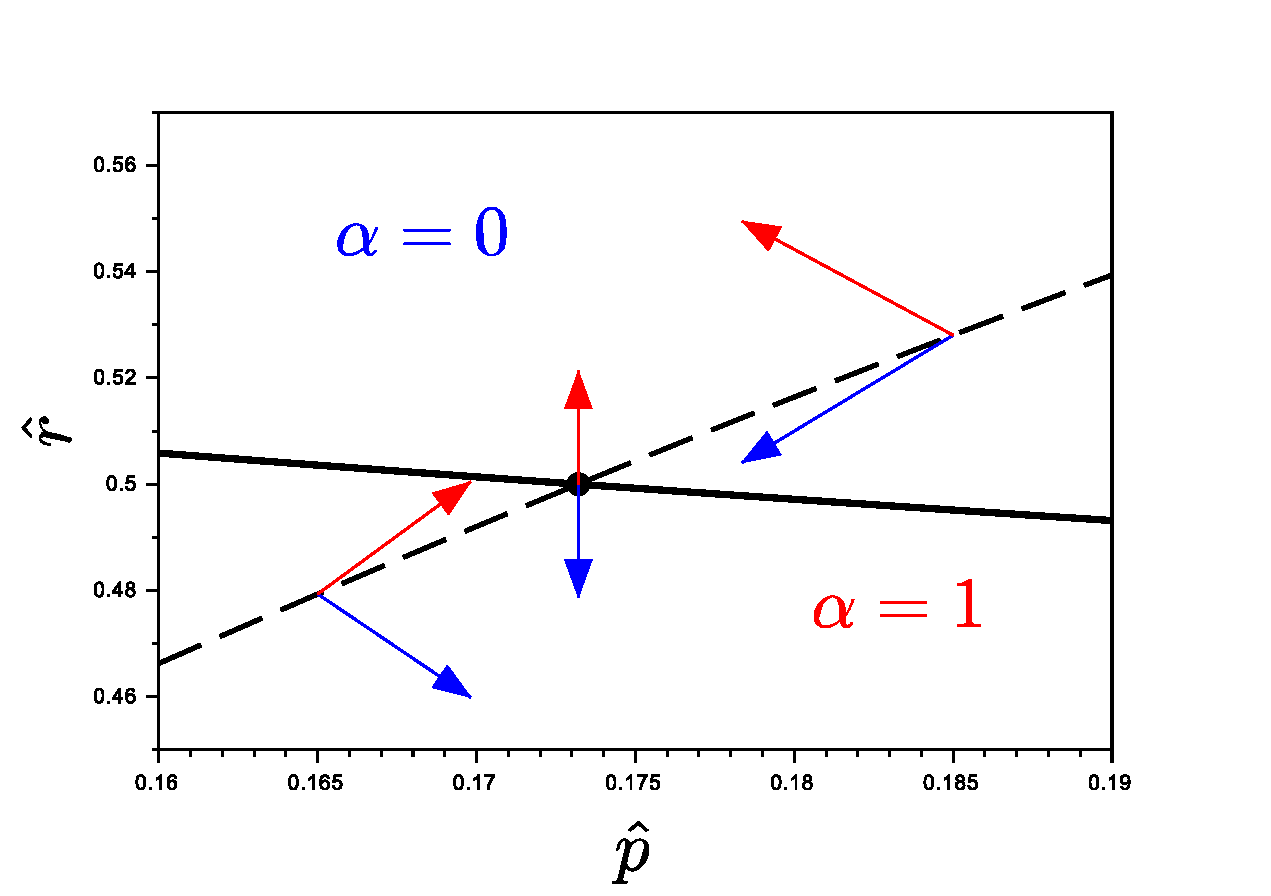
\includegraphics[width=0.8\textwidth]{Fig/Fig_sliding}
\caption
{
\textbf{Local stability of the on-off strategy.}
The on-off strategy sets $\alpha$ to a value of 0 (1) when $\hat{r} > g(\hat{p})$ ($\hat{r} < g(\hat{p})$).
The solid, black curve is the $\hat{p}$-nullcline.
The dashed, black curve is the curve $\hat{r}=g(\hat{p})$.
The arrows represent the vector fields for $\alpha=0$ (in blue) and $\alpha=1$ (in red).
The intersection of the $\hat{p}$-nullcline and the curve $\hat{r}=g(\hat{p})$ corresponds to a unique non-trivial stable steady state, which is equal to $(\hat{p}_{opt}^*, \hat{r}_{opt}^*)$ by Eq.~\ref{eq:supp_adim_h}.
}
\label{fig:sliding}
\end{figure}

\clearpage

\subsection{S2 Text -- Model parameters}
\manuallabel{S2_Text}{S2~Text}

Most of the conclusions of this paper are parameter-independent in the range of physically admissible values.
The exact parameter values used in the simulations aim to represent relevant orders of magnitude.
They were derived from the available literature on fast-growing bacteria (mostly \textit{Escherichia coli}).
This document describes this derivation for each parameter.
In the \textit{Methods} section of the main text, we also describe how some of them were validated by fitting the model to available experimental data (Fig.~\ref{fig:model_validation} in the main text).

The model parameters (Eqs.~\ref{eq:pdef}-\ref{eq:rdef} in the main text) are listed in the table below:
\begin{center}
\begin{tabular}{|c|c|l|}
\hline
Name & Unit & Description \\
\hline
$e_M$ & h$^{-1}$ & Constant characterizing nutrient composition of medium\\
\hline
$k_R$ & h$^{-1}$ & Rate constant of macromolecular synthesis\\
\hline
$K_R$ & g\ L$^{-1}$ & Half-saturation constant of macromolecular synthesis\\
\hline
$\beta$ & L\ g$^{-1}$ & Inverse of the cellular density of macromolecules\\
\hline
$\alpha$ & -- & Resource allocation parameter\\
\hline
\end{tabular}
\end{center}
The values derived below are summarized in \ref{S1_Table}.


\subsubsection{\Large \texorpdfstring{$e_M$}{eM}}

By definition, $e_M$ is the effective turnover of the metabolic macroreaction producing precursors from external substrates, obtained by dividing the reaction rate $v_M$ by the enzyme concentration $m$ (Eq.~\ref{eq:metaflux}).
The unit of $e_M$ is min$^{-1}$, and can be decomposed as follows:
\[
[e_M]  = \frac{\text{[mass of metabolic product]}}{\text{[mass of enzyme M]}\cdot \text{[time]}} = \frac{1}{\text{[time]}}.
\]
Note that $e_M = k_M\, s / (K_M + s)$ where $k_M$ is a rate constant, indicating the maximal rate of conversion of external nutrients to precursor metabolites. 
$e_M$ will thus vary with the concentration $s$ of the external nutrients and the kind of nutrient. 
For example, the precursor mass that can be produced from 1 g of glucose is higher than that produced from 1 g of acetate.

How can we find a typical value for $k_M$, and thus for $e_M$ (both have the same order of magnitude if we suppose that the reaction is not operating far below saturation, that is, $e_M \approx k_M$)?
A reasonable estimate for $k_M$ can be obtained from the turnover numbers of reactions involved in the synthesis of charged tRNA, since the latter are directly consumed by the most abundant part of the gene expression machinery, the ribosomes.

Ref.~\cite{uter_longrange_2004} provides a typical value for such a reaction, catalyzed by glutaminyl-tRNA synthetase: $k_{\textit{cat,GlnRS}} = 3.2$~s\textsuperscript{-1}, indicating that on average 3.2 glutaminyl-tRNA molecules are produced per glutaminyl-tRNA synthetase molecule per second. 
After conversion to mass units using molar weight from~\cite{freist_glutaminyltrna_1997}, this yields
\[
k_{\textit{cat,GlnRS}} = \frac{3.2 \cdot 147}{64.4 \cdot 10^ 3} \approx 10^{-3} \, \text{g of glutaminyl-tRNA} \cdot \text{g of enzyme}^{-1} \cdot \text{s}^{-1}.
\]
We therefore take
\[
k_M \approx 3.6 \text{ h}^{-1},
\]
and thus obtain an upper bound for $e_M$ in our simulations.

\subsubsection{\Large \texorpdfstring{$k_R$}{kR}}

$k_R$ is the mass rate constant describing the maximal rate of conversion of precursors to macromolecules [h\textsuperscript{-1}].
As for $e_M$, we can decompose this into
\[
[k_R]  = \frac{\text{[mass of macromolecules]}}{\text{[mass of gene expression machinery]}\cdot \text{[time]}} = \frac{1}{\text{[time]}}
\]
To obtain an order of magnitude for the mass of macromolecules, we focus on proteins since they are the most abundant macromolecules in the cell~\cite{ehrenberg_mediumdependent_2012}.
The dimensional analysis of $k_R$ thus becomes:
\[
\begin{aligned}
\left[k_R\right] &= \frac{\text{[protein mass produced]}}{\text{[ribosomal mass]} \cdot \text{[hour]}}\\
&= \frac{\text{[moles of protein]} \cdot \text{[protein molar mass]}}{\text{[moles of ribosome]} \cdot \text{[ribosome molar mass]} \cdot \text{[hour]}}\\
&= \frac{\text{[moles of amino acids]} \cdot \text{[molar mass of amino acids]}}{\text{[moles of ribosome]} \cdot \text{[hour]} \cdot \text{[ribosome molar mass]}}\\
&\approx \frac{\text{[maximal protein elongation rate]} \cdot \text{[molar mass of amino-acids]}}{\text{[ribosome molar mass]}}.
\end{aligned}
\]
The values in the last equality are available from the literature~\cite{ehrenberg_mediumdependent_2012,klumpp_molecular_2013,hachiya_increase_2007,yamamoto_mass_2006}.
We obtain
\[
k_R \approx \frac{10 \cdot 100}{10^6}\cdot 3600 \approx 3.6 \text{ h}^{-1}.
\]
This value is comparable with the translational capacity $k_T$, in $\mu$g of protein per $\mu$g of ribosomal protein per hour, given by Scott \textit{et al.}~\cite{scott_interdependence_2010}:
\[
k_T = \frac{4.5 \text{ }\mu\text{g of protein} \text{ / }\mu\text{g of RNA} \text{ / h }}{0.76 \text{ }\mu\text{g of ribosomal protein} \text{ / } \mu\text{g of RNA}} = 5.9 \text{ h}^{-1}.
\]

\subsubsection{\Large \texorpdfstring{$K_R$}{KR}}

A value for the parameter $K_R$, representing the half-saturation constant of macromolecular synthesis, is more difficult to obtain from the literature.
However, assuming that ribosomes operate close to saturation (80\% over a range of growth rates~\cite{ehrenberg_mediumdependent_2012}), we find that $K_R \approx 0.25\,p$, with p the total amino acid concentration.
The total concentration of amino acids in the cell is around 150~mmol~L\textsuperscript{-1}~\cite{bennett_absolute_2009}, which with a mean molecular weight of 118.9~g~mol\textsuperscript{-1} for amino acids~\cite{hachiya_increase_2007}, yields a mass concentration of 17.8~g~L\textsuperscript{-1}.
These considerations led to the following order of magnitude for $K_R$:
\[
K_R \approx 1\text{ g L}^{-1}.
\]

\subsubsection{\Large \texorpdfstring{$\beta$}{Beta}}

$\beta$ is the inverse of the cellular density of macromolecules, which has been shown constant during balanced growth over a large range of growth rates~\cite{churchward_macromolecular_1982}, and there is some data suggesting that $\beta$ varies little during growth transitions as well~\cite{zhou_carbon_2013}.
From~\cite{zimmerman_estimation_1991,mcguffee_diffusion_2010} we take the following typical value for $\beta$:
\[
\beta \approx \frac{1}{300} \approx 0.003 \text{ L g}^{-1}.
\]

\subsubsection{\Large \texorpdfstring{$E_M$}{EM} and \texorpdfstring{$K$}{K}}

From the values of the parameter in the dimensional model, one can deduce the parameters in the nondimensional model used in the simulations:
\[
E_M = \frac{e_M}{k_R} = \frac{3.6}{3.6} = 1 \;\;\;\;\; , \;\;\;\;\;  K = \beta\, K_R = 3\cdot 10^{-3} \cdot 1 = 0.003.
\]

\clearpage

\subsection{S3 Text -- Solution of optimal control problem}
\manuallabel{S3_Text}{S3~Text}

\subsubsection{Statement of the problem}

We consider the dimensionless system defined by Eqs~\ref{eq:pdefnondim}-\ref{eq:rdefnondim} in the main text, which are here repeated for clarity:
\begin{equation}{\label{eq:model}}
\begin{aligned}
\frac{d\hat{p}}{d\hat{t}} &= (1-\hat{r})\, E_M - (1+\hat{p})\, \hat{r} \, \frac{\hat{p}}{K+\hat{p}}, \\
\frac{d\hat{r}}{d\hat{t}} &= \hat{r} \frac{\hat{p}}{K + \hat{p}} \, (\alpha (\hat{t}) - \hat{r}).
\end{aligned}
\end{equation}

As stated in the section \textit{Biomass maximization as an optimal control problem} in the main text, the objective of this study is to maximize the growth rate on an interval $[0,\tau]$ after a nutrient upshift. With Eq.~\ref{eq:supp_growthrate_adim} in \ref{S1_Text}, we have
 
\begin{equation*}
\hat{\mu}= \hat{r}\, \dfrac{\hat{p}}{K+\hat{p}}.
\end{equation*}
In order to avoid boundary effects occurring over finite time intervals, notably the depletion of precursors just before $\tau$, we solve the optimal control problem over an infinite horizon ($\tau \rightarrow \infty$). Consider the set of admissible controls
\[
\mathcal{U}=\{\alpha:\mathbb{R} \rightarrow [0,1] \ \mid \ \alpha(\cdot) \ \mathrm{measurable}\}.
\]
The optimization problem can then be stated as follows:
\begin{equation}\label{Prob}
\alpha_{opt} = \arg \max_{\alpha \in \mathcal{U}} J(\alpha)\equiv \int_0^{+\infty} \hat{r}(\hat{t}) \frac{\hat{p}(\hat{t})}{K + \hat{p}(\hat{t})} d\hat{t} ,
\end{equation}
where $(\hat{p}(\hat{t}),\hat{r}(\hat{t}))$ is the unique solution of Eq.~\ref{eq:model} starting at a given point $(\hat{p}_0,\hat{r}_0)\in \Omega \equiv \mathbb{R}^+_* \times (0,1)$ for a given control $\alpha\in \mathcal{U}$.

Given that the performance index $J(\alpha)$ diverges, we actually consider \textit{overtaking optimality}~\cite{carlson_infinite_1991}.
Consider the performance index of the trajectory $x(\cdot)$ emanating from $x_0$ and generated by $u(\cdot)$ defined for any $T\geq 0$ by
$$
J_T(x_0,u(\cdot))=\int_0^T f_0(x(t),u(t),t)dt.
$$
A trajectory $x^*(\cdot)$ emanating from $x_0$ and generated by $u^*(\cdot)$ is said to be overtaking optimal if for any other trajectory $x(\cdot)$ emanating from $x_0$ and generated by $u(\cdot)$ the following holds
$$
\liminf_{T\rightarrow\infty} \left\lbrace J_T(x_0,u^*(\cdot)) - J_T(x_0,u(\cdot))\right\rbrace\geq 0.
$$
Roughly speaking, a trajectory is overtaking optimal if "the performance index catches up with the performance index of any other trajectory"~\cite{carlson_infinite_1991}.

\subsubsection{Maximum Principle}

Necessary conditions on optimal trajectories can be obtained by the Infinite Horizon Maximum Principle~\cite{carlson_infinite_1991}.
Let $H(\hat{p},\hat{r},\lambda_p,\lambda_r,\lambda_0,\alpha)$ be the Hamiltonian of the system, defined by
\[
H(\cdot) \equiv \lambda_p\, E_M\, (1-\hat{r}) - \hat{r}\, \dfrac{\hat{p}}{K+\hat{p}}\left[\lambda_p (1+\hat{p}) +\lambda_r\, \hat{r} +\lambda_0\right] + \alpha \, \lambda_r \, \hat{r}\, \frac{\hat{p}}{K+\hat{p}}.
\]
Moreover, let $\alpha$ be an optimal control, and $\hat{x}(\cdot)=(\hat{p}(\cdot),\hat{r}(\cdot))$ the associated trajectory.
Then, there exists $\lambda_0 \leq 0$ and an absolutely continuous map $\lambda=(\lambda_p,\lambda_r):[0,+\infty) \rightarrow \mathbb{R}^2$
such that $(\lambda,\lambda_0)\neq0$, and
\begin{align}
\dot{\lambda}_p\, =-\frac{\partial H}{\partial \hat p}&= \hat{r} \, \frac{K}{(K+\hat{p})^2}\, \left[\lambda_p \, (1+\hat{p}) +\lambda_r\, ( \hat{r}-\alpha) + \lambda_0\right] + \hat{r}\, \frac{\hat{p}}{K+\hat{p}}\, \lambda_p, \label{eq:adjoint_p}\\
 \dot{\lambda}_r\, =-\frac{\partial H}{\partial \hat r}&= \lambda_p\, E_M +\frac{\hat{p}}{K+\hat{p}} \, \left[\lambda_p \, (1+\hat{p}) +\lambda_r\, (2 \hat{r}-\alpha) +\lambda_0\right] \label{eq:adjoint_r}.
\end{align}
The maximization condition is given by:
\begin{equation}{\label{eq:PMP}}
\begin{aligned}
&\alpha(\hat{t}) \in \arg\ max_{v \in [0,1]} H(\hat{x}(\hat{t}),\lambda(\hat{t}),\lambda_0,v), \\ &\mathrm{almost}\ \mathrm{everywhere}\ \mathrm{on}\ [0,+\infty).
\end{aligned}
\end{equation}

An extremal trajectory is a quadruplet $(\hat{x}(\cdot),\lambda(\cdot),\lambda_0,\alpha(\cdot))$ satisfying Eqs~\ref{eq:model}-\ref{eq:PMP}. The extremal is said to be normal (resp. abnormal) if $\lambda_0<0$ (resp. $\lambda_0=0$). In the normal case, we normalize the adjoint vector so that $\lambda_0=-1$.

From Eq.~\ref{eq:PMP}, it follows that the control strategy is given by the sign of the \textit{switching function} $\phi(\cdot) \equiv \lambda_r \, \hat{r}\, \hat{p}/(K+\hat{p})$, that is,
\[
\begin{cases}
\alpha=1 \iff \phi(\cdot) >0,\\
\alpha=0 \iff \phi(\cdot)<0.
\end{cases}
\]

Finally, given that the system is autonomous, the Hamiltonian is conserved along any extremal trajectory.

\subsubsection{Characterization of singular arcs}

Whenever $\phi$ is vanishing over a time interval, we say that the trajectory is \textit{singular}.
We will now characterize such trajectories.
If $I=[\hat{t}_1,\hat{t}_2]$ is a singular arc, we have $\phi(\hat{t})=\dot{\phi}(\hat{t})=0$, for all $\hat{t}\in[\hat{t}_1,\hat{t}_2]$, that is, $\lambda_r(\hat{t})=0$ and $\dot\lambda_r(\hat{t})=0$. 

For abnormal extremal trajectories, we get $\lambda_p(\hat{t})=0$, in contradiction with the Maximum Principle, so there is no singular arc. An abnormal extremal trajectory is therefore a concatenation of bang arcs.

For normal extremal trajectories, using additionally that $H$ is constant along an extremal trajectory, we obtain that $\lambda_p$ is constant along a singular arc. By combining $\dot \lambda_p=0$ and $\dot \lambda_r=0$, we obtain $\hat{p}(\hat{t})=\sqrt{E_M\, K}=\hat{p}_{opt}^*$. Using $d\hat{p}/d\hat{t}=0$, we finally get $\hat{r}(\hat{t})=\hat{r}_{opt}^*$.
Thus, the singular arc is the optimal steady state, corresponding to a singular control $\alpha(\hat{t})=\alpha_{opt}^*$, with $\alpha_{opt}^*$ depending on $E_M$ (\ref{S1_Text}).

A necessary condition of optimality for a singular arc is given by the Kelley condition~\cite{borisov_fullers_2000}.
We must differentiate $\phi$ with respect to $\hat{t}$ until $\alpha$ appears in the derivative. Along a singular arc, we obtain for $q=2$:
\[
(-1)^q \; \frac{\partial}{\partial\alpha} \; \frac{d^{2q}}{d\hat{t}^{2q}} \; \phi(\hat{t})<0,
\]
satisfying the Kelley condition necessary for optimality. Given that the singular arc is of second order, an optimal trajectory can enter into the singular arc only by a \textit{chattering arc} (also called the Fuller's phenomenon, \textit{i.e.}, an arc with an infinite number of switches~\cite{borisov_fullers_2000,marchal_chattering_2013}).

\subsubsection{Analysis of the adjoint system}

Recalling that a switch corresponds to a change of sign of $\lambda_r$, the analysis of the adjoint system (Eqs~\ref{eq:adjoint_p}-\ref{eq:adjoint_r}) may be useful to characterize the switches of extremal trajectories. 

First, for the abnormal case, we can easily determine in the phase-plane the possible transitions between the four regions defined by the axes (see Fig.~\ref{fig-adj}). A trajectory can cross at most twice the $\lambda_p$-axis, so  we conclude that an abnormal extremal cannot have more than two switches. Thus, an abnormal extremal is a concatenation of at most three bang arcs ($\alpha(t)=0$ or $\alpha(t)=1$). When  $\alpha(t)=0$ or $\alpha(t)=1$ for a long time, the growth rate tends to zero. We therefore conclude that  abnormal extremal trajectories are not optimal.

Secondly, for the normal case, after the first switch, a trajectory with two consecutive switches in the regions $\{(\hat{p},\hat{r})\in \Omega \mid \hat{p}<\hat{p}_{opt}^*\}$ or $\{(\hat{p},\hat{r})\in \Omega \mid \hat{p}>\hat{p}_{opt}^*\}$ is not possible, as shown in Fig.~\ref{fig-adj}. Therefore, such a trajectory is not optimal given that it does not fulfill the conditions given by the Maximum Principle.
We conclude that if the optimal trajectory has a concatenation of bang arcs, the switches must alternatingly occur in the regions  $\{(\hat{p},\hat{r})\in \Omega \mid \hat{p}<\hat{p}_{opt}^*\}$ and $\{(\hat{p},\hat{r})\in \Omega \mid \hat{p}>\hat{p}_{opt}^*\}$.

\begin{figure}[tb]
\centering
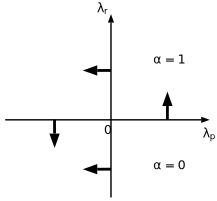
\includegraphics[height=4cm]{Fig/adj2ab} 
\includegraphics[height=4cm]{Fig/adj2} 
\caption{\textbf{Transitions between regions in the phase-plane for the adjoint system.} A switch occurs when a trajectory crosses the $\lambda_p$-axis. Left: abnormal case. An extremal trajectory cannot have more than two switches. Right: normal case. $(\lambda_p^s,0)$ corresponds to the singular arc.  After the first switch, an extremal trajectory cannot have two consecutive switches if it stays in the region $\{(\hat{p},\hat{r})\in \Omega \mid \hat{p}<\hat{p}_{opt}^*\}$ or $\{(\hat{p},\hat{r})\in \Omega \mid \hat{p}>\hat{p}_{opt}^*\}$.}
\label{fig-adj}                               
\end{figure} 


\subsubsection{Optimal trajectories}

From the Maximum Principle, we have shown that the optimal trajectory is a concatenation of bang arcs ($\alpha(t)=0$ or $\alpha(t)=1$) and possibly a singular arc corresponding to the optimal steady state $(\hat{p}(\hat{t}),\hat{r}(\hat{t}))=(\hat{p}_{opt}^*,\hat{r}_{opt}^*)$. Moreover, if the optimal trajectory has a singular arc, it must enter it through a chattering arc (\textit{i.e.}, with an infinite number of switches between $\alpha=0$ and $\alpha=1$).

These elements motivate the supposition that optimal solutions consist in a transient (chattering arc) towards the optimal steady state, after which they remain there (until the next change of environment). The chattering arc can be characterized by a switching curve $\hat{p}\mapsto\varphi(\hat{p})$ which passes through the optimal steady state.
Defining $A_0$ and $A_1$ the regions above and below $\varphi$ in the $(\hat{p},\hat{r})$-plane, respectively, we conjecture that the following feedback control law is optimal: 
%The simplest way to reach the optimal steady-state is thus two arcs, either 0-1 or 1-0 depending on the initial conditions. More precisely, let $\phi_0$ and $\phi_1$ be defined as the the trajectories solution of System \eqref{model} backward in time starting at $(p_{opt}^*,r_{opt}^*)$ with respectively $\alpha=0$ and $\alpha=1$. Given $\phi=\phi_0 \cup \phi_1$, we define $A_0$ and $A_1$ the regions above and below $\phi$ in the plane $(p,r)$. 


\begin{equation}\label{control-opt}
\begin{cases}
\alpha(\hat{t})=0 \ \textrm{if} \ (\hat{p}(\hat{t}),\hat{r}(\hat{t}))\in A_0,\\
\alpha(\hat{t})=1 \ \textrm{if} \ (\hat{p}(\hat{t}),\hat{r}(\hat{t}))\in A_1,\\
\alpha(\hat{t})=\alpha_{opt} \ \textrm{if} \ (\hat{p}(\hat{t}),\hat{r}(\hat{t}))=(\hat{p}_{opt}^*,\hat{r}_{opt}^*).
\end{cases}
\end{equation}


Loosely speaking, the chattering arc corresponds to a spiral composed of bang arcs wrapping around the optimal steady state, where the switches alternatingly occur in the regions  $\{(\hat{p},\hat{r})\in \Omega \mid \hat{p}<\hat{p}_{opt}^*\}$ and $\{(\hat{p},\hat{r})\in \Omega \mid \hat{p}>\hat{p}_{opt}^*\}$, in line with the analysis of the adjoint system.
This is a first hint that the proposed control strategy is optimal. Moreover, our conjecture is also in line with the \textit{turnpike property}:
Trélat and Zuazua~\cite{trelat_turnpike_2015} have shown that, for quite a generic class of systems, the optimal strategy consists in staying at the optimal steady state (after a short transient).

As explained in the \textit{Methods} section of the main text, we numerically solved the optimal control problem by the direct method using the \texttt{bocop} software~\cite{bonnans_bocop_2012}. 
It is important to stress that the optimization process was performed without any preliminary assumptions on the characteristics of the optimal trajectory. 
The fact that the numerical solution verifies the Maximum Principle (\textit{i.e.}, the singular arc corresponds to the optimal steady state) and the Kelley condition (\textit{i.e.}, the presence of a chattering arc)
tends to confirm that the control strategy of Eq.~\ref{control-opt} is optimal. As an aside, we note that due to the fact that numerical optimization was performed for a finite horizon, we actually obtained a second chattering arc escaping from the singular arc at the end of the simulation.  This is a classical property of the turnpike strategy: the optimal trajectory leaves the optimal steady state just before the end of the time interval of interest, in our case consuming almost all precursors. This arc was removed from the plot in Fig.~\ref{fig:optimalcontrol}, because it does not occur with an infinite horizon and is therefore a numerical artifact for this study.

\clearpage

\subsection[S4 Text -- Kinetic model of the ppGpp system]{S4 Text -- Kinetic model of the ppGpp system in \textit{Escherichia coli}}
\sectionmark{Kinetic model of the ppGpp system}
\manuallabel{S4_Text}{S4~Text}

The recently published model of Bosdriesz \textit{et al.}~\cite{bosdriesz_how_2015} provides a synthesis of the currently available knowledge of the ppGpp regulatory system.
Through the mechanisms of ppGpp production and degradation, it describes regulation of the synthesis of ribosomal RNA.
We explain below how we use the model to compare the action of the ppGpp system with the on-off control strategy.
The denomination of variables and parameters follows the Supporting Information of~\cite{bosdriesz_how_2015} , and is reproduced in Table~\ref{tab:notations} in order to make the text self-contained.

The evolution of the cellular concentration of ppGpp is described in~\cite{bosdriesz_how_2015} by
\begin{equation}
\label{eq:ppGpp}
\frac{d\texttt{ppGpp}}{dt} = v_{RelA}(r_{t,tot}) + v_{spoT} - k_{spoT} \cdot \texttt{ppGpp},
\end{equation}
where $v_{spoT}$ and $k_{spoT}$ are constants (see Table~\ref{tab:notations}), and $v_{RelA}$ is a function of $r_{t,tot}$, the total concentration of "stalled" ribosomes:
\begin{equation}
\label{eq:vrelA}
v_{RelA}(r_{t,tot}) = k_{RelA} \cdot RelA_{tot} \cdot \frac{r_{t,tot}}{K_{D,RelA} + r_{t,tot}}.
\end{equation}
The amount of stalled ribosomes is determined by the equilibrium between charged and uncharged tRNA, $t_{ai}$ and $t_{i}$, in the cell:
\begin{equation}
\label{eq:rttot}
r_{t,tot} = \sum_i r_{ti} = \sum_i r_i \frac{t_i/\kappa_{t}}{1+t_{ai}/\kappa_{ta}+t_i/\kappa_{t}},
\end{equation}
which can be rewritten as
\begin{equation}
\label{eq:rttot-f}
r_{t,tot} = \sum_i r_i \frac{t_i/\kappa_{t}}{1+(0.5 r-t_i)/\kappa_{ta}+t_i/\kappa_{t}},
\end{equation}
using the assumption that $t_{tot,i}  = t_{ai} + t_i = 0.5 \cdot r$.
$r_i$ denotes the concentration of ribosomes recognizing amino acid  $i$.
Finally, with $r = \sum_i r_i$ the total ribosome concentration and $a_i$ the concentration of amino acid $i$, the dynamics of the charged tRNA concentration is described by
\begin{equation}
\label{eq:ti_dynamic}
\frac{dt_{ai}}{dt} = v_{tai}(a_i, t_{i}) - f_i \cdot v_{ribosome}(t_i,r),
\end{equation}
with $v_{tai}(a_i, t_{i})$ the synthesis rate of charged tRNA, and $f_i \cdot v_{ribosome}(t_i,r)$ their consumption via protein synthesis.
In particular,
\begin{eqnarray}
v_{tai}(a_i, t_{i}) &=& k_{Si} \cdot S_{tot,i} \cdot \frac{t_i\, a_i}{t_i\,  K_{Mai} + a_i\,  K_{Mti} + t_i\,  a_i}, \label{eq:vtai}\\
v_{ribosome}(t_i, r) &=& k_{rib} \cdot r \cdot \left(1+ \sum_i \left[ f_i \cdot \left( 1 + \frac{t_i}{\kappa_t} \right) \frac{\kappa_{ta}}{0.5\cdot r - t_i} \right]\right)^{-1}. \label{eq:vrib}
\end{eqnarray}

For comparison with our framework, we need $\texttt{ppGpp}$ as a direct function of the total amino acid concentration $a = \sum_i a_i$ (a proxy for precursors) and total ribosome concentration $r$ (a proxy for gene expression machinery).
To this end, we made two additionnal assumptions:
\begin{description}
\item[(A1)] All concentrations specific to one type of amino acid $i$ ($a_i$, $t_{ai}$, $t_{i}$, $r_i$) are in the same proportion $f_i = f = 1/20$ with respect to the total concentrations ($a$, $t_{a}$, $t$, $r$).
\item[(A2)] We apply a quasi-steady-state approximation (QSSA) to the dynamics of the concentration of the charged tRNAs ($t_{ai}$) and the concentration of ppGpp ($\texttt{ppGpp}$).
That is, the dynamics of these variables are assumed fast relative to the dynamics of the amino acid concentrations ($a_i$) and the total ribosome concentration ($r$).
\end{description}
Using (A2), we can rewrite Eq.~\ref{eq:ti_dynamic} as follow:
\begin{equation}\label{eq:vtai_vrib}
v_{tai}(a_i, t_{i}) = f_i \cdot v_{ribosome}(t_i,r),
\end{equation}
which, using (A1) and Eqs~\ref{eq:vtai} and \ref{eq:vrib}, leads to:
\begin{equation}
\label{eq:vtai_vrib_without_sum}
k_{Si} \cdot S_{tot,i} \cdot \frac{t_i\, a_i}{t_i\, K_{Mai} + a_i\, K_{Mti} + t_i\, a_i}
= f_i \cdot k_{rib} \cdot r \cdot
  \left(1 + \frac{\kappa_{ta}}{0.5 r - t_i} \cdot \left( 1 + \frac{t_i}{\kappa_t} \right)  \right)^{-1}.
\end{equation}
By rearranging both sides of the equation, $t_i$ can be expressed as a function of $a_i$ and $r$, which yields:

\begin{equation}
\begin{alignedat}{2}
&A {t_i}^2 + B t_i + C = 0, \;\;\; \text{with}\\
&A = \frac{k_{Si} \,S_{tot,i} \,a_i}{f_i\, k_{rib} \,r} \left( \frac{\kappa_{ta}}{\kappa_t} - 1\right) + K_{Mai} + a_i,\\
&B = \frac{k_{Si} \,S_{tot,i} \,a_i}{f_i \,k_{rib} \,r} (0.5\,r+\kappa_{ta}) + a_i \,K_{Mti} - 0.5\,r\,(K_{Mai} + a_i),\\
&C = - 0.5 \,r \,a_i \,K_{Mti},
\end{alignedat}
\end{equation}
and therefore
\[
t_i (a_i, r) = \frac{-B \pm \sqrt{B^2 - 4AC}}{2A}.
\]
It is not difficult to show that the only solution on $[0, 0.5\,r]$ is
\begin{equation}
\label{eq:ti_final}
t_i (a_i, r) = \frac{-B + \sqrt{B^2 - 4AC}}{2A}.
\end{equation}
From this result, we obtain $r_{t,tot}$ as a function of $a_i$ and $r$, by applying (A1) to Eq.~\ref{eq:rttot-f}:
\begin{equation}
\label{eq:rttot-f_without_sum}
r_{t,tot}(t_i, r) = r \cdot \frac{t_i/\kappa_{t}}{1+(0.5 r-t_i)/\kappa_{ta}+t_i/\kappa_{t}},
\end{equation}
and substituting $t_i$ by the expression of Eq.~\ref{eq:ti_final}.

Finally, we apply (A2) to Eq.~\ref{eq:ppGpp} and obtain the final expression giving the concentration of ppGpp as a function of the total amino acid and ribosome concentrations:
\begin{equation}
\texttt{ppGpp}(a_i, r) = \frac{1}{k_{spoT}} \left( k_{RelA} \cdot RelA_{tot} \cdot \frac{r_{t,tot}(a_i, r)}{K_{D,RelA} + r_{t,tot}(a_i,r)} + v_{spoT} \right).
\end{equation}
This function is represented in Fig.~\ref{fig:ppGpp} with parameters taken from Table~\ref{tab:notations}.

The plotted surface of the function resembles the inverse of the on-off control strategy in Fig.~\ref{fig:ppGppsurface}, as expected, bearing in mind that ppGpp has an inhibitory effect on the synthesis of ribosomal RNA.
We assumed a Michaelis-Menten inhibition for the regulatory effect of ppGpp on rRNA synthesis, and thus indirectly on the synthesis of ribosomal proteins~\cite{potrykus_pppgpp_2008,keener_regulation_1996}:
\begin{equation}
\alpha (\texttt{ppGpp}) = \frac{K_I}{K_I + \texttt{ppGpp}}.
\end{equation}
The inhibitory constant $K_I$ lies in the dynamical range of variation of $\texttt{ppGpp}$.
In Fig.~\ref{fig:ppGppsurface} in the main text, we took $K_I = 10$~$\mu$M.

\begin{figure}[p]
\centering
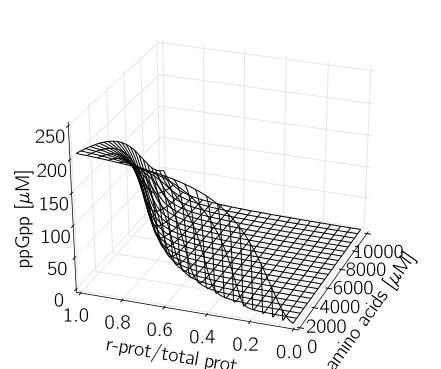
\includegraphics[width=0.7\textwidth]{./Fig/FigS4-1}
\caption[ppGpp concentration is a function of total ribosome and amino acid concentrations.]
{
{\bf ppGpp concentration is a function of total ribosome and amino acid concentrations.}\newline
We assume the dynamics of ppGpp to be fast on the time-scale of changes in the ribosome and amino acid concentrations.
The concentration of ppGpp can thus be expressed as a function of the latter two variables, using the model of Bosdriesz \textit{et al.}~\cite{bosdriesz_how_2015}.
Parameters are taken from Table~\ref{tab:notations}.
}
\label{fig:ppGpp}
\end{figure}

\begin{table}[p]
\scriptsize
\centering
\begin{tabular}{cccl}
\hline
\hline
\textbf{Symbol} & \textbf{Value} & \textbf{Unit} & \textbf{Description} \\
\hline
\hline
$a_i$ & -- & $\mu$M & Concentration of aa $i$ (not incorporated in protein)\\

$t_{ai}$ & -- & $\mu$M & Concentration of tRNA charged with aa $i$\\

$t_{i}$ & -- & $\mu$M & Concentration of free tRNA conjugate to aa $i$\\

$t_{tot,i}$ &  $0.5 \cdot r$ & $\mu$M & Total concentration of tRNA conjugate to aa $i$\\

$r_{i}$ & -- & $\mu$M & Total concentration of ribosome with an A-site for aa $i$\\

$r_{ti}$ & -- & $\mu$M & Ribosomes with uncharged tRNA in an A-site for aa $i$\\

$\texttt{ppGpp}$ & -- & $\mu$M & Concentration of ppGpp\\
\hline
$a$ & $\sum_i a_{i}$ & $\mu$M & Total concentration of aa (not incorporated in protein)\\

$t_{a}$ & $\sum_i t_{ai}$ & $\mu$M & Total concentration of tRNA charged with aa\\

$t$ & $\sum_i t_{i}$ & $\mu$M & Total concentration of free tRNA\\

$r_{t,tot}$ & $\sum_i r_{ti}$ & $\mu$M & Total concentration of uncharged tRNA bound to ribosomes\\

$r$ & $\sum_i r_i$ & $\mu$M & Total concentration of ribosomes\\
\hline
$v_{RelA}$ & -- & $\mu$M/s & Rate of RelA-catalyzed ppGpp synthesis\\

$v_{SpoT}$ & $10^{-3}$ & $\mu$M/s & Rate of ppGpp synthesis by SpoT\\

$v_{tai}$ & -- & $\mu$M/s & Rate of amino-acyl tRNA $i$ synthetase\\

$v_{ribosome}$ & -- & $\mu$M/s & Total rate of protein synthesis\\
\hline
$k_{rib}$ & 20 & s\textsuperscript{-1} & $k_{cat}$ of protein elongation\\

$k_{RelA}$ & 75 & s\textsuperscript{-1} & $k_{cat}$ of ppGpp synthesis by RelA\\

$K_{D,RelA}$ & 0.26 & $\mu$M & Michaelis constant of RelA-catalyzed ppGpp production\\

$RelA_{tot}$ & 1/15 & $\mu$M & RelA concentration\\

$k_{SpoT}$ & $\ln (2) / 30$ & s\textsuperscript{-1} & Rate of ppGpp degradation by SpoT\\

$\kappa_t$ & 500 & $\mu$M & Dissociation constant of uncharged tRNA-ribosome complex\\

$\kappa_{ta}$ & 1 & $\mu$M & Dissociation constant of charged tRNA-ribosome complex\\

$k_{Si}$ & 100 & s\textsuperscript{-1} & $k_{cat}$ of aminoacyl-tRNA synthetase\\

$S_{tot,i}$ & 1 & $\mu$M & Total concentration of aminoacyl-tRNA synthetase for aa $i$\\

$K_{Mai}$ & 100 & $\mu$M & Michaelis constant of aa-tRNA synthetase for amino acids\\

$K_{Mti}$ & 1 & $\mu$M & Michaelis constant of aa-tRNA synthetase for uncharged tRNA\\

$f_i$ & 1/20 & -- & Proportion of aa $i$ in proteins (Assumption A1)\\

\end{tabular}
\caption{\textbf{Parameters and variables reused from Bosdriesz \textit{et al.}~\cite{bosdriesz_how_2015}}. The abbreviation aa denotes amino acids.}
\label{tab:notations}
\end{table}

\clearpage

\subsection{S1 Table -- Parameter values of self-replicator model}
\manuallabel{S1_Table}{S1~Table}

\begin{table}[h]
\centering
\begin{tabular}{|c|c|c|c|}
\hline
Parameter & Unit & Literature value & Fitted value \\
\hline
$\gamma$ & $-$ & No value & 1.39\\
\hline
$k_R$ & h$^{-1}$ & 3.6 & 2.23\\
\hline
$e_M$ for M63+glycerol & h$^{-1}$ &  $< 3.6$ & 0.587\\
\hline
$e_M$ for M63+glucose & h$^{-1}$ &  $< 3.6$ & 0.867\\
\hline
$e_M$ for cAA+glycerol & h$^{-1}$ &  $< 3.6$ & 1.07\\
\hline
$e_M$ for cAA+glucose & h$^{-1}$ &  $< 3.6$ & 1.57\\
\hline
$e_M$ for RDM+glycerol & h$^{-1}$ &  $< 3.6$ & 3.48\\
\hline
$e_M$ for RDM+glucose & h$^{-1}$ &  $< 3.6$ & 4.76\\
\hline
$\beta K_R$ & $-$  & 0.003 & Not fitted\\
\hline
\end{tabular}
\caption{\textbf{Parameter values of self-replicator model}
The parameter values in the model were obtained by fitting Eq.~\ref{eq:alpha_mu_optimal_dim} to the data of Scott et al~\cite{scott_interdependence_2010} (Fig.~\ref{fig:model_validation} in the main text), as described in the \textit{Methods} section. They are compared with order-of-magnitude estimates from the literature (\ref{S2_Text}).}
\end{table}

\clearpage

\subsection{S1 Figure -- Simple control strategies for the self-replicator of bacterial growth}
\manuallabel{S1_Fig}{S1~Figure}

\begin{figure}[h]
\centering
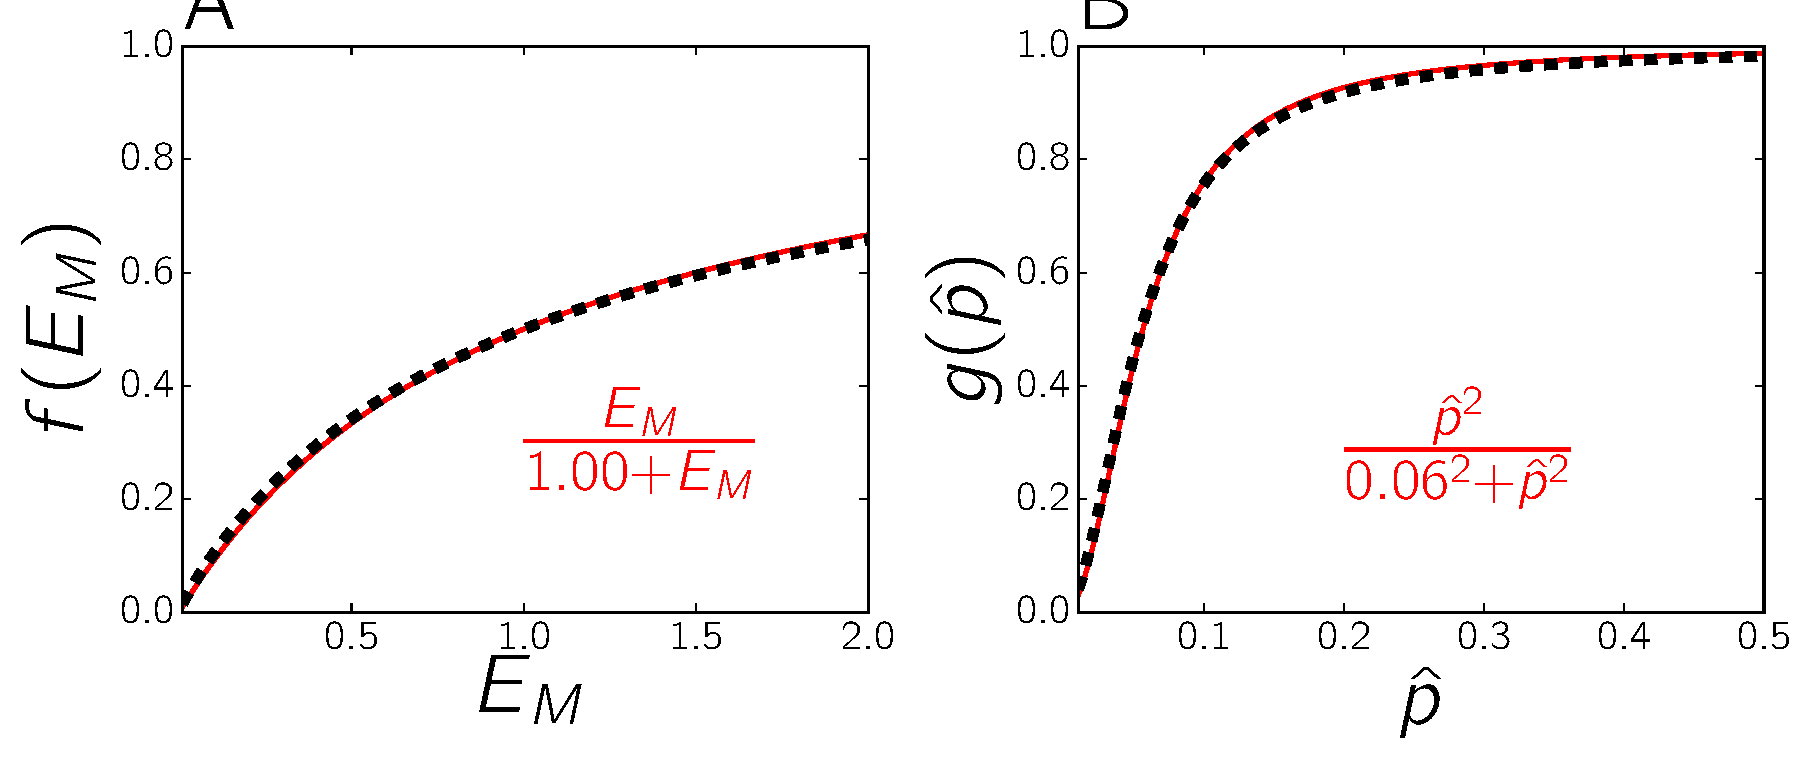
\includegraphics[width=\textwidth]{./Fig/plot_strategies}
\caption{
\noindent\textit{A:} Nutrient-only strategy: $\alpha = f(E_M)$.
The dashed, black curve is the (unique) strategy driving the system exactly to the optimal steady state, that is, the state in which growth occurs at the maximal rate supported by $E_M$.
The function $f$ is defined by Eq.~\ref{eq:meth_f} in the \textit{Methods} section of the main text.
The solid, red curve is an approximation of this function by the simple Michaelis-Menten curve of Eq.~\ref{eq:MMApprox}, with $K_{mE} = 1.0$.
\textit{B:} Precursor-only strategy: $\alpha = g(\hat{p})$.
The dashed, black curve is the (unique) strategy driving the system exactly to the optimal steady state.
The function $g$ is defined by Eq.~\ref{eq:meth_g} in the \textit{Methods} section of the main text.
The solid, red curve is an approximation of this function by the simple Hill curve of Eq.~\ref{eq:HillApprox}, with $K_{mp} = 0.06$ and a cooperativity coefficient 2.}
\end{figure}

\chapter{Dynamics of the gene expression machinery during an acetate-glucose upshift}
\chaptermark{Gene expr. machinery during an upshift}
\label{chap:experiments}

%\textit{"If reality does not fit the concept, too bad for reality."} -- Georg Wilhelm Friedrich Hegel

\selectlanguage{french}
\section*{Résumé en français du Chapître \thechapter : Dynamique de la machinerie d'expression génique lors d'une transition acétate vers glucose.}

Résumé d'environ 6-8 paragraphes (2 pages).
\selectlanguage{english}

\section{Introduction}

Most studies of the growth of microorganisms have been done at steady state.
This is a reasonable and logical choice given that at steady state, the behavior of microorganisms is reproducible, which helps uncovering simple theories to apprehend their inherent complexity.
But while this condition can be easily achieved in the laboratory, microorganisms naturally spend very little time in steady state.
This motivated the construction of a new theoretical framework in Chapter~\ref{chap:theory} to study growth laws during growth transitions.

The principles underlying regulatory processes in dynamical conditions appear to be different from those applying at steady state.
We showed that regulatory strategies approaching the theoretical optimal, given by bang-bang control of gene expression machinery, have to be able to effect abrupt and strong variations in the activity of a gene.
It was seen that for implementing such strategies the regulatory system needs to be capable of sensing the internal state of the cell and not just the environment.
A near-optimal transition also requires information of several different variables, whereas for maintaining a steady state with maximal biomass accumulation a single variable turned out to be sufficient in our theoretical framework.
Interestingly, we showed that the ppGpp regulatory system of \textit{E. coli} fulfills the requirement of such a regulatory strategy, by implementing an on-off strategy for regulating the synthesis of ribosomes.
However, although this provides circumstantial evidence that bacteria control resource allocation in a manner consistent with theoretical optimality, experimental data are necessary to decide if an on-off strategy is at work in \textit{E. coli} during growth transitions.

Unfortunately, far more information is available on ribosome abundance at steady state than during growth transitions~\cite{scott_interdependence_2010,gausing_regulation_1980}.
The main reason for this bias on steady-state conditions is that, from an experimental point of view, growth transitions are hard to control and may depend on the history of the culture~\cite{ng_damage_1962,dufrenne_effect_1997,shaw_effect_1967,mcmeekin_predictive_2002,cheroutre-vialette_application_2002}.
However, as we discussed in Section~\ref{sec:discussion}, the few studies that have been reported seem to be consistent with our predictions, in the sense that they indicate that during growth transitions, the synthesis rate of ribomoses oscillates~\cite{gausing_regulation_1980,zengel_transcription_1986} and the ppGpp concentration manifests a rapid succession of increases and decreases~\cite{friesen_synthesis_1975,murray_control_2003}.
But we cannot decisively validate or disprove the model predictions from measurements that were carried out at the population level, where it is inherently hard to identify switching patterns.
What is needed for the verification of our predictions are dynamical single-cell measurements of the ribosome concentration during well-controlled growth transitions.
While the observation of an on-off strategy would show that simple models of the type introduced in Chapter~\ref{chap:theory} are instrumental in gaining a better understanding of microbial physiology, its refutation would also raise interesting questions. 
If maximization of growth rate and biomass accumulation have been retained by natural selection in \textit{E. coli}, which factors would prevent the cell from behaving optimally from a theoretical point of view?

The aim of this chapter is to measure \textit{in vivo}, during a growth transition, the resource allocation profile $\alpha (\cdot)$ and compare its dynamics with the gold standard established in Chapter~\ref{chap:theory}.
To this end, we have measured ribosomal abundance of \textit{E. coli} at the single-cell level during a nutrient upshift.
More precisely, we constructed a strain in which a fluorescent marker has been attached to a ribosomal subunit, thus allowing the \textit{in-vivo} monitoring of (changes in) the abundance of ribosomes.
In collaboration with Irina Mihalcescu of the Laboratoire Interdisciplinaire de Physique, we cultivated this \textit{E. coli} strain in a microfluidic device, allowing the long-term imaging of individual cells in well-controlled conditions, notably involving a classic upshift experiment from growth in minimal medium with acetate to minimal medium with glucose.
We then developed a Kalman smoothing method, in collaboration with Eugenio Cinquemani of Inria Grenoble -- Rh\^{o}ne-Alpes, to reconstruct $\alpha (\cdot)$  from the estimates of the variations of the growth rate and the relative ribosomal synthesis rate.
While the preliminary results presented here do not allow a decisive validation of the expected behavior, among other things due to the difficulties that were encountered during the experiments and the image analysis, we believe they are promising as a first step towards the better understanding of global resource allocation during growth transitions.

For clarity, the model of resource allocation during growth transitions developed in Chapter~\ref{chap:theory} is reproduced here, where dotted variables represent time derivatives:
\begin{eqnarray}
\dot{p}(t) &=& e_M(t)\cdot (1/\beta - r(t)) - \frac{k_R \cdot p(t)}{K_R + p(t)}\cdot r(t) \, (1+\beta\, p(t)), \label{eq:pdef-exp}\\
\dot{r}(t) &=& \frac{k_R \cdot p(t)}{K_R + p(t)}\cdot r(t) \, (\alpha(t) - \beta\, r(t)). \label{eq:rdef-exp}
\end{eqnarray}
In this form, it contains 4 variables ($e_M(t)$, $p(t)$, $r(t)$, $\alpha (t)$) and 3 parameters ($\beta$, $k_R$, $K_R$).
$e_M(t)$ [min\textsuperscript{-1}] is an indicator of the richness of the environment.
$p(t)$ [g.L\textsuperscript{-1}] is the precursor concentration inside the cell.
$r(t)$ [g.L\textsuperscript{-1}] is the concentration of gene expression machinery inside the cell.
$\alpha (t)$ [$\emptyset$] is the fraction of resources allocated to the synthesis of gene expression machinery.
$k_R$ [min\textsuperscript{-1}] is the rate constant of macromolecular synthesis.
$K_R$ [g.L\textsuperscript{-1}] is the half-saturation constant of macromolecular synthesis.
$\beta$ [L.g\textsuperscript{-1}] is the inverse of the cellular density of macromolecules, assumed to be constant.



\section{Results}

\subsection{Experimental design}
\label{sec:exp_design}

How can one measure the resource allocation variable in \textit{E. coli} cells?
There is no direct way to quantify $\alpha (\cdot)$ in an experiment, mostly because of its abstract nature.
To correctly reconstruct it, one has to know the value of every single term in the equations in which it appears.
In the model of Eqs~\ref{eq:pdef-exp}-\ref{eq:rdef-exp}, $\alpha$ only appears in Eq.~\ref{eq:rdef-exp}.
We can therefore identify $\alpha (t_k)$ for each time $t_k$ when the terms $\beta r(t_k)$, $\dot{r}(t_k)$, and $\frac{k_R \cdot p(t_k)}{K_R + p(t_k)} \cdot r(t_k)$ are known, or equivalently, the six individual components $r(t_k)$, $\dot{r}(t_k)$, $p(t_k)$, $k_R$, $K_R$, $\beta$ they are composed of.
Even when assuming that the parameters $k_R$, $K_R$, and $\beta$ are known, or at least easy to estimate independently, reconstructing the dynamics of $\alpha$ would require estimation of the (changes in) concentration of the gene expression machinery ($r$, $\dot{r}$) and the precursor concentration $p$.

Are such measurements feasible in practice?
The abundance of ribosomes can be quantified, for instance, by measuring the total RNA of the cell~\cite{scott_interdependence_2010}, or using radioactive markers \cite{gausing_regulation_1980,zengel_transcription_1986}, fluorescent labels~\cite{bakshi_superresolution_2012}, or mass spectrometry techniques~\cite{hui_quantitative_2015}.
However, only the use of fluorescent proteins complies with our need for real-time single-cell quantification.
Obtaining an estimate of precursor abundance is even more challenging, since there is no clear proxy for the totality of precursors in the cell and, while absolute quantification of all internal metabolites has been achieved in \textit{E. coli}~\cite{bennett_absolute_2009}, this method is also not suitable for a dynamical estimation in individual cells.

The problem of quantifying $\alpha (\cdot)$ can be simplified by applying a transformation of the model of Eqs~\ref{eq:pdef-exp}-\ref{eq:rdef-exp}.
Taking into account that by construction the growth rate $\mu(t)$ is given by
\[
	\mu (t) = \beta \frac{k_R \cdot p(t)}{K_R + p(t)} \cdot r(t),
\]
we can rewrite Eq.~\ref{eq:rdef-exp} as follows
\begin{equation}
\label{eq:dot_r}
\dot{r}(t) = \mu (t) \, \left(\frac{\alpha(t)}{\beta} - r(t) \right).
\end{equation}
The problem of estimating $\alpha(\cdot)$ is thus equivalent to the problem of estimating $r(\cdot)$, $\dot{r}(\cdot)$, $\mu (\cdot)$ and $\beta$.
If we are satisfied with estimating $\alpha$ up to a constant factor $\beta$, dynamically measuring the ribosome concentration and the growth rate would make $\alpha (\cdot) / \beta$ identifiable. 

Given that fluorescent reporters of ribosomal proteins can provide information on both $r(\cdot)$ and $\dot{r}(\cdot)$ \cite{zulkower_robust_2015}, the above reformulation of the problem is promising for the purposes of our study.
Moreover, since the predicted bang-bang profiles in gene activity are easily hidden at the population level if cells are not synchronous, which is generally the case, expression of the ribosomal genes need to be monitored at high sampling density on the single-cell level, which is also possible with fluorescent reporters.
Inspired by previous work~\cite{bakshi_superresolution_2012}, we therefore constructed an \textit{E. coli} strain in which the S2 ribosomal subunit, encoded by the gene \textit{rpsB}, has been tagged with a green fluorescent protein (GFP).
The strain with the chromosomal \textit{rpsB-gfp} fusion produces fluorescent ribosomes that are quantifiable \textit{in vivo} in single cells while not affecting the growth rate (see Material and Methods~\ref{sec:methods_strain} and~\cite{bakshi_superresolution_2012}).
Monitoring single cells of this strain, by time-lapse fluorescence microscopy, thus makes it possible to estimate $r(\cdot)$ and $\dot{r}(\cdot)$ and reconstruct $\mu(\cdot)$.

The growth conditions also need to be carefully chosen for this study.
In natural environments, for many bacteria one of the most frequently encountered growth transitions, or at least the transition on which selection is expected to operate, is the transition from stationary phase in a nutrient-deprived medium~\cite{gefen_direct_2014} to (exponential) growth after the renewed availability of nutrients.
The transition from stationary to exponential phase is difficult to study though as many hard-to-control parameters play a role, including the duration of the nutrient stress, the composition of the medium before growth arrest, and the accumulation of waste products in the medium~\cite{ehrenberg_mediumdependent_2012}.
As a consequence, growth resumption only occurs after a lag phase of variable duration~\cite{ng_damage_1962,dufrenne_effect_1997,shaw_effect_1967,mcmeekin_predictive_2002,cheroutre-vialette_application_2002}, which is not included in the model.
For this reason, we decided to focus on a transition from exponential growth on a poor carbon source (acetate) to exponential growth on a rich carbon source (glucose) in a well-defined minimal medium.
By construction, this steady-state-to-steady-state transition requires a long acquisition time before and after the shift, respectively, to ensure that the cells have no memory of their physiological state before the transition and have enough time to reach the new steady state after the transition.
The use of the mother machine, a microfluidic device that was designed to sustain exponential growth for long periods of time, is therefore a good choice for this purpose.
It allows to maintain a constant flow of fresh medium and to effect fast transitions by switching the medium (see Material and Methods~\ref{sec:growth_condition} and \ref{sec:microflu}).
The complete experimental plan is summarized in Fig.~\ref{fig:experiment_schema}.

\begin{figure}[tb]
\centering
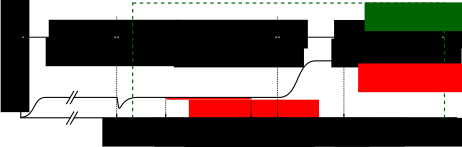
\includegraphics[scale=1]{./Fig/experiment_schema}
\caption{
\textbf{Schematic outline of the upshift experiment.}
The goal is to measure the fluorescence and length/area of \textit{E. coli} \textit{rpsB-gfp} cells during an acetate-to-glucose upshift.
We use M9 minimal medium supplemented with 0.2\% of acetate or glucose (see Material and Methods~\ref{sec:growth_condition}).
A preculture was started from glycerol stock for 2.5 days on 0.2\% acetate in batch condition (shake flask).
The day of the experiment, the cells were injected into the mothermachine and fed by a constant flow of fresh 0.2\% acetate medium (see Material and Methods~\ref{sec:microflu}).
Fluorescence and phase contrast images were taken every 5 minutes.
After 20~h, the feeding media was switched to 0.2\% glucose and maintained for 20~h while continuing image acquisition.
Time 0 corresponds to the moment of the acetate-glucose upshift.
}
\label{fig:experiment_schema}
\end{figure}

\subsection{Data acquisition}
\label{sec:data_acquisition}

An experiment following the plan of Fig.~\ref{fig:experiment_schema} was carried out, over a period of 40~h, but encountered a number of difficulties.
First, the motor displacing the microscope along the Z-axis intermittently stalled, thus deactivating the autofocus and the Z-compensation for the tilt of the microfluidic device in the XY plane.
As a consequence, until the experimenter manually intervened, many of the images acquired were out of focus.
This is the reason why data points between -720 and -150 min are not exploitable, but fortunately the experiment was planned in such a way that when it really mattered, notably around the growth transition, someone was present to monitor the microscope.
Second, at around 7~h after the nutrient upshift, the bacteria started to die for reasons that are unknown, the most plausible hypothesis being a phage contamination (see Discussion~\ref{sec:chap3_discussion}).
Data analysis was therefore limited to 550 min after the upshift, when roughly 3/4 of the cells were still growing.
For these and other reasons (see Section~\ref{sec:chap3_discussion}), the experiment will have to be repeated, but there was no time left for this in the framework of my PhD thesis.

The acquired data consisted of phase contrast and fluorescence images of 60 wells in total, in four different fields.
While quite a few image analysis programs have been reported in the literature~\cite{klein_tlm-tracker:_2012,wang_image_2010,young_measuring_2012,paintdakhi_oufti:_2016}, and some of these specifically address the mother machine design of the microfluidic device~\cite{wang_robust_2010,sachs_image-based_2016}, they all presented limitations when applied to our data.
For instance, the segmentation algorithms experienced difficulties due to the low resolution of the camera, and the phase contrast images had a superposed reflection band due to the microfluidic device.
Moreover, the fluorescence density was concentrated in hot spots (Fig.~\ref{fig:data_acquisition}) and its intensity varied during the experiment. 
While this was expected, since ribosomes are localized in the cell poles~\cite{bakshi_superresolution_2012} and ribosomal abundance is known to vary with the growth rate~\cite{scott_interdependence_2010}, it complicated automatic segmentation on the fluorescence images.

For these reasons, the image analysis carried out for this chapter has been much simplified. 
First, we have focused on the cell at the bottom of each well, since this avoids the tracking of individual cells across several generations and ensures that the descendance of this cell can be followed throughout the experiment.
Second, segmentation was done by manually selecting two pixels, one at each pole of the cell.
These pixels were used to create a rectangle surrounding the cell (Fig.~\ref{fig:data_acquisition} and Material and Methods~\ref{sec:cell_segmentation}).
After background correction (Material and Methods~\ref{sec:cell_segmentation}), the fluorescence intensity in units RFU was evaluated for each pixel in the rectangle, as well as the length of the cell, defined by the distance in pixels between the poles (Fig.~\ref{fig:data_acquisition}).
The fluorescence density for the entire cell [RFU/pixel/cell] was computed by dividing the sum of the fluorescence intensities of the pixels in the rectangle by the total number of pixels in the rectangle.
Although we are well aware that the above procedure can be improved on many counts (Section~\ref{sec:chap3_discussion}), we nevertheless believe that it provides a reasonable approximation of the quantities of interest and a valid starting-point for the estimation of the growth rate and the resource allocation profile in the remainder of this chapter.   


\begin{figure}[p]
\centering
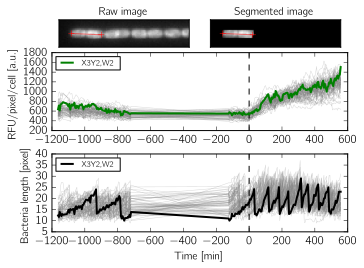
\includegraphics[scale=1]{./Fig/data_acquisition}
\caption{
\textbf{Results of data acquisition.}
We imaged 6 fields (X[1-3]Y[1-2]) each containing 15 wells (W[0-14]) for $\sim$40~h.
From the 90 wells, 68 were suitable for further analysis (the others being empty, out of frame for some period of time, or plugged).
For all wells, data points are missing in the interval between [-720,-150] because the camera was out of focus.
We stopped the analysis at 550~min, when about 3/4 of the bacteria were still growing, before the entire population died within a few hours for an unknown reason.
The image labeled "Raw image" is the last image analyzed for the highlighted well.
The bacterium on the left of this image was manually segmented by selecting two pixels at the poles on the fluorescence images (red cross).
A 6-pixel-wide rectangular mask was computed for each image, resulting in the "Segmented image" on the right.
Fluorescence intensities are expressed in Relative Fluorescence Units (RFU) on a 16-bit image and were corrected for camera background, but not autofluorescence background (Material and Methods~\ref{sec:cell_segmentation} and Discussion~\ref{sec:chap3_discussion}).
The fluorescence intensity of the cell, expressed in units RFU/pixel/cell, was computed by dividing the sum of the fluorescence intensities of the pixels in the rectangle by the total number of pixels in the rectangle.
The cell length is the distance in pixels between the two poles (red line).
The thick lines in green and black highlight the time-varying length and fluorescence density for the cell visible in the top images, labeled "X3Y2, W2".
The vertical dashed lines represent the time of the upshift from growth on acetate to growth on glucose.
}
\label{fig:data_acquisition}
\end{figure}

In total, we obtained time courses of fluorescence density [RFU/pixel/cell] and the length for 68 bacterial cells (Fig.~\ref{fig:data_acquisition}).
The fluorescence density appears constant during growth on acetate (before time 0) and immediately increases when the carbon source is switched to glucose.
Inspection of the cellular length shows that the division frequency abruptly increases after the nutrient upshift, corresponding to a higher growth rate.
Unfortunately, while steady-state growth on acetate was reached before the upshift, the fluorescence density profile suggests that the experiment did not continue long enough to ensure that a new steady state on glucose was reached.
However, the data before and after the nutrient upshift are exploitable.
What do we observe if we estimate the growth rate and the resource allocation profile from these data?

\subsection{Data analysis using Kalman smoothing}
\label{sec:res_kalman}

As we presented in section~\ref{sec:exp_design}, our goal is to reconstruct the signal $\alpha (\cdot)$ during a growth transition.
By modeling \textit{E. coli} as a cylinder, the volume can be assumed directly proportional to the length of the cell.
If we assume a negligible background of autofluorescence (see Material and Methods~\ref{sec:cell_segmentation}), the fluorescence concentration in the cell can be assumed proportional to the ribosome concentration.
More precisely, based on the available data, we have the following measurement model at each time-point $t_k$, $0\leq k \leq N-1$:
\begin{eqnarray}
L(t_k) &= \lambda \cdot V(t_k) + \epsilon_k, \label{eq:mes_L}\\
F(t_k) &= \gamma \cdot r(t_k) + \eta_k, \label{eq:mes_F}
\end{eqnarray}
where $L(t_k)$ and $F(t_k)$ are the length and fluorescence density in units RFU/pixel measured at time $t_k$, respectively,  and $V(t_k)$  and $r(t_k)$ the corresponding actual volume and ribosome concentration at time $t_k$, respectively. ($\lambda$,$\gamma$) are unknown proportionality constants, and ($\epsilon_k$,$\eta_k$) uncorrelated sequence of measurement noise assumed normally distributed with mean 0.

As explained in Section~\ref{sec:exp_design}, reconstructing $\alpha (\cdot)$ requires information on $\mu (\cdot)$, $r(\cdot)$ and $\dot{r}(\cdot)$.
From Eq.~\ref{eq:mes_F}, we can obtain $r(\cdot)$ and $\dot{r}(\cdot)$ by smoothing interpolation and differentiation.
Similarly, $\mu (\cdot)$ can be derived from Eq.~\ref{eq:mes_L} as it is defined by
\[
\dot{V}(t) = \mu (t) \cdot V(t).
\]
However, smoothing interpolation is particularly sensible to the boundary conditions.
Since each division in the time series generates a new boundary condition, smoothing interpolation of our data is expected to be little robust.
For this reason, the growth rate of single cells is usually estimated by fitting an exponential function to the volume data between each cell~\cite{wang_robust_2010,izard_synthetic_2015}.
While this is suitable when bacteria are at steady state, it is not applicable during a growth transition, where we expect the growth rate to vary between successive divisions.
Other techniques are less sensible to the above problem~\cite{zulkower_robust_2015}, and we decided to use Kalman smoothing for our purpose~\cite{kailath_linear_2000,jazwinski_stochastic_2007}.

Kalman filtering~\cite{kalman_new_1960} is a Bayesian algorithm using a series of noisy measurements to predict the state of a dynamical system.
It has been extensively used in engineering applications (guidance, tracking, control, ...) requiring the real-time estimation of hidden variables in a dynamical system from present and past measurements.
Kalman smoothing is an extension of Kalman filtering using information about past and present but also future measurements of the state of the system, and is widely applied to estimate unknown inputs in time series analysis~\cite{kailath_linear_2000,jazwinski_stochastic_2007}.
The advantage of Kalman filtering with respect to Kalman smoothing is that it uses all available information to estimate the hidden variables of a dynamical system, in applications where a real-time response is not required.
For our problem, at each time step $t_k$, our hidden variables are the resource allocation variable $\alpha (t_k)$ and the growth rate $\mu (t_k)$, while the available information consists of the $N$ measurements $\left\{ F(t_0), F(t_1), ..., F(t_{N-1}) \right\}$ and $\left\{L(t_0), L(t_1), ..., L(t_{N-1}) \right\}$ that were taken during the experiment.

The Kalman filtering problem can now be formulated as follows.
The state of a growing bacterial cell is described by the dynamical system
\begin{eqnarray}
\dot{r}(t) &=& \mu (t) \cdot \frac{\alpha(t)}{\beta} - \mu (t) \cdot r(t),\\
\dot{V}(t) &=& \mu (t) \cdot V(t),
\end{eqnarray}
with initial conditions $r(0) = r_0$, $V(0) = V_0$, and the following measurement model:
\begin{eqnarray}
L(t_k) &= \lambda \cdot V(t_k) + \epsilon_k,\\
F(t_k) &= \gamma \cdot r(t_k) + \eta_k,
\end{eqnarray}
where the variables are as defined as for Eqs~\ref{eq:dot_r}, \ref{eq:mes_L} and \ref{eq:mes_F}.
While $\beta$ can be obtained from the literature (Chapter~\ref{chap:theory}), $\lambda$ and $\gamma$ are unknown parameters that need to be estimated along with $\alpha (\cdot)$ and $\mu (\cdot)$.
Since we are satisfied with a qualitative reconstruction of $\alpha (\cdot)$, we can simplify the system by defining $r_\gamma = \gamma \cdot r$ and $V_\lambda = \lambda \cdot V$.
The dynamical system is consequently rewritten as
\begin{eqnarray}
\dot{r}_\gamma(t) &=& \mu (t) \cdot\frac{\gamma \cdot \alpha(t)}{\beta} - \mu (t) \cdot r_\gamma (t),\label{eq:r_prob}\\
\dot{V}_\lambda (t) &=& \mu (t) \cdot V_\lambda (t),\label{eq:V_prob}
\end{eqnarray}
with initial conditions $r_\gamma (0) = \gamma r_0$, $V_\lambda (0) = \lambda V_0$, and the new measurement model:
\begin{eqnarray}
F(t_k) &= r_\gamma (t_k) + \eta_k,\label{eq:F_prob}\\
L(t_k) &= V_\lambda(t_k) + \epsilon_k.\label{eq:L_prob}
\end{eqnarray}
The Kalman filtering problem thus becomes the reconstruction of $\gamma \alpha (\cdot) / \beta$ and $\mu (\cdot)$ from measurements $\left\{ F(t_0), ..., F(t_{N-1}) \right\}$ and $\left\{L(t_0), ..., L(t_{N-1}) \right\}$.

Note that the above problem is not linear, whereas Kalman filtering was initially introduced for linear systems~\cite{kalman_new_1960,kailath_linear_2000}.
For this reason, we use a nonlinear extension of Kalman smoothing called unscented Kalman smoothing~\cite{julier_new_1997,jazwinski_stochastic_2007}.
Details about its exact implementation are available in Material and Methods~\ref{sec:meth_kalman}.
While it is feasible to simultaneously reconstruct the signals $\mu (\cdot)$ and $\gamma \alpha (\cdot) / \beta$ using Kalman smoothing, it is not necessary in our case and might lead to unstable results.
We therefore decided to proceed in two steps: first reconstruct $\mu(\cdot)$ from the measurements $L(\cdot)$, than inject this result into the reconstruction of $\gamma \alpha(\cdot) / \beta$ from the measurements $F(\cdot)$.

\subsection{Estimation of growth rate and resource allocation profile}
\label{sec:estim_gr_ra}

\subsubsection*{Growth rate estimation}

As presented in the previous section, we want to reconstruct the growth rate $\mu$ defined by Eq.~\ref{eq:V_prob}, using measurements of the length $L$ defined by Eq.~\ref{eq:L_prob}.
Note that Kalman smoothing is a procedure that returns the expected mean and covariance of the state of a dynamical system, given the  measurements.
Therefore, reconstructing $\mu$ requires it to be explicitly included as a state variable of the dynamical system.
This provides constraints on the variation of $\mu$ that have the effect of a regularization.
In particular, in the Kalman smoothing procedure, we model the variations of $\mu$ as the outcome of a stochastic process.
The laws describing this process play the role of a prior on the expected regularity of $\mu$ (the more noisy the process, the less constrained the variations of $\mu$).
In particular, we define $\mu$ as the double integral of a Gaussian white noise $w$:
\[
\dot{\mu} = v(t), \;\;\;\; \dot{v} = w(t),
\]
where $v$ is an intermediate variable and $w(t)$ is assumed normally distributed with mean 0 and standard deviation $\theta$: $w(t) \sim \mathcal{N}(0, \theta)$.
The resulting system then becomes
\begin{eqnarray}
\dot{V_\lambda}(t) &=& \mu (t) \cdot V_\lambda (t),\nonumber\\
\dot{\mu}(t) &=& v(t),\label{eq:full_mu_prob}\\
\dot{v}(t) &=& w(t),\nonumber
\end{eqnarray}
with the measurement model
\begin{equation}
L(t_k) = V_\lambda(t_k) + \epsilon_k,
\end{equation}
and the initial conditions
\[
V_\lambda (0) = V_{\lambda,0}, \;\;\;\; \mu (0) = \mu_0 , \;\;\;\; v(0) = v_0,
\]
that may themselves be Gaussian random variables with some given statistics.
The advantages of this regularization method are that the reconstructed $\mu$ is guaranteed to be second-order differentiable.
It is also equivalent to other methods like Tikhonov regularization~\cite{tikhonov1977solutions,tikhonov1963solution,de_nicolao_nonparametric_1997}, which minimizes least-square differences between predictions and observations along with penalizing the variations of the input.

Our prior is thus entirely contained in the parameters of the Kalman procedure:
\begin{itemize}
\item the mean of the initial state $(V_{\lambda,0}, \mu_0, v_0)$,
\item the covariance of the initial state $(V_{\lambda,0}, \mu_0, v_0)$,
\item the transition covariance for the derivatives of $V_\lambda$, $\mu$ and $v$ (see below),
\item the variance of the observation noise $\epsilon_k$.
\end{itemize}
The mean and covariance of the initial state $(V_{\lambda,0}, \mu_0, v_0)$ represent the knowledge we have of the initial values of the variables.
For instance, if we know exactly the initial value of the growth rate $\mu$ (\textit{via} independent measurements or literature data), we can use it as mean for $\mu_0$ along with a very small variance.
This will constraint the signal reconstruction by penalizing deviations from this value at $t=0$.
On the contrary, if we are very uncertain of the value for $V_{\lambda,0}$ (because cells are not synchronized, and can be in any state when the data acquisition starts), we can use a large variance for this initial condition.
In our framework, there is no transition covariance for $V_\lambda$ and $\mu$, because they are not the result of a stochastic process (the equations that define their derivatives are fully deterministic).
However, by definition $v$ is the result of a stochastic process of mean 0 and transition variance $\theta^2$.
This value is crucial and represents the intensity of the white noise $w$ that serves as prior for the regularization of $\mu$.
The smaller its value, the more the variations of $v$ are penalized, hence the smoother the reconstructed $\mu (\cdot)$.
Finally, the variance of the observation noise $\epsilon_k$ is simply the expected measurement noise.
Together, these parameters represents the \textit{prior} information we have on the initial conditions, the smoothness of the reconstructed signal, and the precision of our measurements, in order to reconstruct the growth rate $\mu (\cdot)$.
As we will see below, we widely use these properties to overcome the difficulties introduced by the discontinuities following cell divisions.

The observation of the length $L$ of growing bacterial cells is inherently discontinuous, due to the division of cells at regular time-points (Fig.~\ref{fig:data_acquisition}).
The estimation problem can therefore not be solved for the experiment as a whole, but only for the time-intervals between two successive division events, when the cell length is expected to change continuously.
We localize the division events by identifying the time points at which the empirical derivative of the length is below an arbitrary threshold, and correspondingly slice the total duration of the experiment into time-intervals with continuous changes of cell length.
The simplest way to proceed from there on would be to treat each portion independently.
However, by doing this we would lose important information, since the growth rates of a mother and its daughter cells are expected to be similar.
In other word, while not necessary continuous, the growth rate of new-born cells will depend strongly on the growth rate of their mother just before division.
This can be easily taken into account in the Kalman smoothing procedure by exploiting the prior information about the initial mean and covariance of the system variables.
In particular, we set the mean of the initial growth rate of a daughter cell equal to the final estimated growth rate of the mother cell, while defining a reasonable variance of the growth rate to allow for uncertainty.
The results of this Kalman smoothing procedure, along with the exact parameters used, are reported in Fig.~\ref{fig:growth_rate_estimation} and Material and Methods~\ref{sec:meth_kalman}.

\begin{figure}[p]
\centering
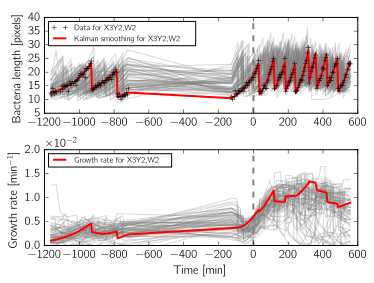
\includegraphics[scale=1]{./Fig/growth_rate_estimation}
\caption{
\textbf{Growth-rate estimation using Kalman smoothing based on measurement of the length of bacteria growing in a microfluidic device.}
Gray lines represent the estimation of the time-varying length (upper plot) and growth rate (lower plot) of 68 cells by the unscented Kalman smoothing procedure.
The solid red lines highlight the result for one particular cell, located at the bottom of the well labelled "X3Y2, W2", while black crosses in the top graph are the data points for this cell.
The vertical dashed lines represent the time of the upshift from growth on acetate to growth on glucose.
As prior for the algorithm, we used an observation variance of 9 pixels\textsuperscript{2} for the length $L$.
The transition variance $\theta^2$ (\textit{i.e.}, the smoothing factor for $\mu$) is fixed at $10^{-8}$~min\textsuperscript{-6}.
Inheritance between mother and daughter cells is taken into account by systematically choosing an initial mean growth rate equal to the last estimated value for $\mu$ before cell division, and to half the last estimated value for $V_\gamma$, bearing in mind that \textit{E. coli} cells divide symmetrically.
At the start of the experiment, when no mother cell is available to provide initial estimates, the above values were fixed at 15~pixels for $V_\gamma$ and 0.004~min\textsuperscript{-1} for $\mu$.
The variances associated with these means are 16~pixels\textsuperscript{2} and $10^{-4}$~min\textsuperscript{-2}, respectively for $V_\gamma$ and $\mu$.
The initial mean of $v$ is set equal to 0, with an initial variance of $10^{-8}$~min\textsuperscript{-6}.
All the cross-covariances are set to 0 because the system variables are independent by construction.
}
\label{fig:growth_rate_estimation}
\end{figure}

On average, the results presented in~Fig.~\ref{fig:growth_rate_estimation} show a roughly constant growth rate on acetate, followed by a quick increase after the upshift.
Contrary to what was visible in the plot with the fluorescence data, a steady state for the growth rate seems to have been reached before the end of the experiment.
When considering the individual cells, the results are more difficult to interpret.
A significant part of the cells stopped growing before the end of the experiment, probably due to the fact that all cells die from an unknown cause around the end of the experiment. 
As a consequence, the analysis has been limited to a time-interval after the upshift in which roughly 3/4 of the cells are still growing.
Interestingly, 1/6 of the cells exhibit growth rate oscillations, with a 1~h-long pause around 200 min after the upshift, followed by a recovery of the growth rate until the end of the experiment (see~\ref{S2_Figure}  and \ref{S3_Figure}).
In order to focus the analysis, we decided to classify the cells in three categories: dying cells (N=12) for which the growth rate drops to zero after the upshift, pausing cells (N=11) for which the growth rate drops to zero after the upshift and then recovers, and finally so-called normal cells (N=45) which do not exhibit any of the above behaviors (see~\ref{S2_Figure} and \ref{S3_Figure})
In what follows, we focus on the 45 normal cells (Fig.~\ref{fig:growth_rate_estimation_median}) which show a globally coherent behavior in the time window considered here.

\begin{figure}[tb]
\centering
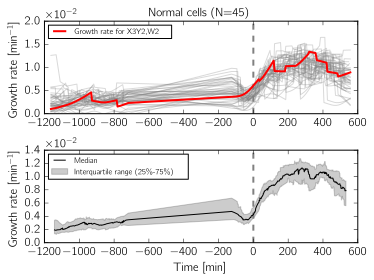
\includegraphics[scale=1]{./Fig/growth_rate_estimation_median}
\caption{
\textbf{Growth-rate estimation using Kalman smoothing for the normal cells only.}
The top graph is the same as the bottom graph of Fig.~\ref{fig:growth_rate_estimation}, except that the dying and pausing cells were removed.
The bottom graph shows the 25\% (lower gray curve), 50\% (solid black curve) and 75\% (upper gray curve) quartiles, computed at each time step.
The gray area represents the interquartile range.
}
\label{fig:growth_rate_estimation_median}
\end{figure}

\subsubsection*{Estimation of resource allocation profile}

In order to estimate the time-varying allocation of resources after the upshift, we use a similar Bayesian regularization approach as for the estimation of the growth rate.
We note $u(t) = \gamma \alpha (t) / \beta$ the resource allocation input that we wish to reconstruct.
With $\hat{\mu}$ the estimation of $\mu$ obtained in the previous section, the full model for the reconstruction of $u (\cdot)$ is given by
\begin{eqnarray}
\dot{r}_\gamma(t) &=& \hat{\mu} (t) \cdot u (t) - \hat{\mu} (t) \cdot r_\gamma (t), \nonumber\\
\dot{u}(t) &=& v(t),\label{eq:full_u_prob}\\
\dot{v}(t) &=& w(t),\nonumber
\end{eqnarray}
with the measurement model
\begin{equation}
F(t_k) = r_\gamma (t_k) + \eta_k,\\
\end{equation}
and the initial conditions
\[
r_\gamma (0) = r_{\gamma,0}, \;\;\;\; u (0) = u_0 , \;\;\;\; v(0) = v_0,
\]
that may themselves be Gaussian random variables with some given statistics.
Contrary to the model used for the estimation of the growth rate, the system of Eq.~\ref{eq:full_u_prob} is linear.
Furthermore, we do not have to deal with discontinuities in the measurements, since the fluorescence density $F$ in the cells is continuous between mother and daughter cells (Fig.~\ref{fig:data_acquisition}).

Given the analysis in Chapter~\ref{chap:theory}, we expect $u(\cdot)$ to exhibit bang-bang variations after the upshift.
This is a discontinuous signal that could be complicated to reconstruct for certain choices of the parameters of the regularization method.
In order to parametrize the Kalman smoothing algorithm, we generated synthetic data by simulating the model of Chapter~\ref{chap:theory}.
We estimated the noise characteristics of $F$ using the RFU/pixel measurements from Fig.~\ref{fig:data_acquisition} (\ref{S7_Text}) and chose parameters that allow the model to reproduce the observed growth rates and fluorescence densities.
We simulated an upshift from acetate to glucose and tried to estimate $\gamma \alpha(\cdot) / \beta$ from these synthetic data, selecting the \textit{prior} in the Kalman smoothing procedure by trial and error.
This approach may not have been optimal for our purpose and possible improvements are discussed in Section~\ref{sec:chap3_discussion}.
The results along with the \textit{prior} used are reported in Fig.~\ref{fig:synthetic_upshift}.
As expected, like any smoothing method, the algorithm has difficulty in reconstructing stiff variations in the state variables of Eq.~\ref{eq:full_u_prob}.
The switching profile of the resource allocation input is relatively well captured though, which indicates that the algorithm is in principle capable of reconstructing an on-off strategy (further improvements are discussed in Section~\ref{sec:chap3_discussion}).
In what follows, we use the same \textit{prior} of the Kalman smoothing procedure for the normal cells identified in the previous section, to test the occurrence of an on-off switching profile in our data.

\begin{figure}[p]
\centering
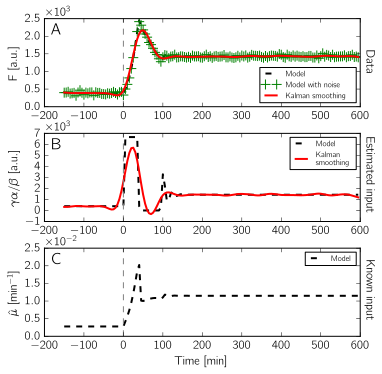
\includegraphics[scale=1]{./Fig/synthetic_upshift}
\caption{
\textbf{Performance of the Kalman smoothing procedure on synthetic data simulating an acetate-glucose upshift.}
\textit{(A)}~Synthetic data simulating an upshift from acetate to glucose, with and without additive white noise, as well as the results obtained by Kalman smoothing.
The synthetic data were generated by simulating the model presented in Eqs~\ref{eq:pdef}-\ref{eq:rdef} with the on-off regulatory strategy (Eq.~\ref{eq:stratswitch} and Fig.~\ref{fig:onoffresults}).
The model parameters used for the simulation are $e_{M,\texttt{Ace}} = 0.18$~h\textsuperscript{-1}, $e_{M,\texttt{Glu}} = 0.9$~h\textsuperscript{-1}, $k_R = 3.6$~h\textsuperscript{-1}, $\beta = 0.003$~L~g\textsuperscript{-1}, $K_R = 1$~g~L\textsuperscript{-1}.
The predicted $r(t)$ profile was multiplied by a factor $\gamma = 0.02$~RFU~L~g\textsuperscript{-1} in order to obtain the corresponding fluorescence intensity profile $F$ (dashed black curve).
The noise level was estimated from the data (\ref{S7_Text}) and added to $F$.
The choice of the parameters of the Kalman smoothing procedure is discussed in the Material and Methods~\ref{sec:meth_kalman}.
\textit{(B)}~Estimation of the resource allocation profile $\gamma \alpha / \beta$ based on the data in \textit{(A)}.
Following Chapter~\ref{chap:theory}, $\alpha (t)$ displays a bang-bang-singular profile during the upshift (dashed black curve).
While the Kalman smoother is not able to capture the discontinuous variations in $\gamma \alpha / \beta$, it qualitatively reproduces the input quite well (red solid curve).
\textit{(C)}~The predicted growth rate during the upshift experiment.
This information is used as an input in the smoothing procedure, since it is supposed to have been independently estimated from the measurements $\left\{L(t_0), ..., L(t_{N-1}) \right\}$.
}
\label{fig:synthetic_upshift}
\end{figure}

The results of the reconstruction of the resource allocation profile $u = \gamma \alpha (\cdot) / \beta$ are presented in Fig.~\ref{fig:gene_activity}.
Within the interval between -150 and 0 min, resource allocation remains more or less stable, as expected for steady-state growth on acetate.
On the contrary, the reconstructed resource allocation profile seems particularly unstable at the beginning and the end of the experiment.
While oscillations do occur after the upshift, these need to be taken with much care.
The problem of reconstructing an on-off strategy is more challenging than we initially thought, for the simple reason that the expected signal is similar to the kind of artifacts a poorly calibrated regularization method would generate.
Data about the pre-upshift and post-upshift steady state are crucial for the calibration of the method and, as explained in Section~\ref{sec:data_acquisition}, the experiment had to be interrupted before a steady state on glucose was attained.
We extensively discuss this and other problems in Section~\ref{sec:chap3_discussion} and give directions for future improvements.

\begin{figure}[p]
\centering
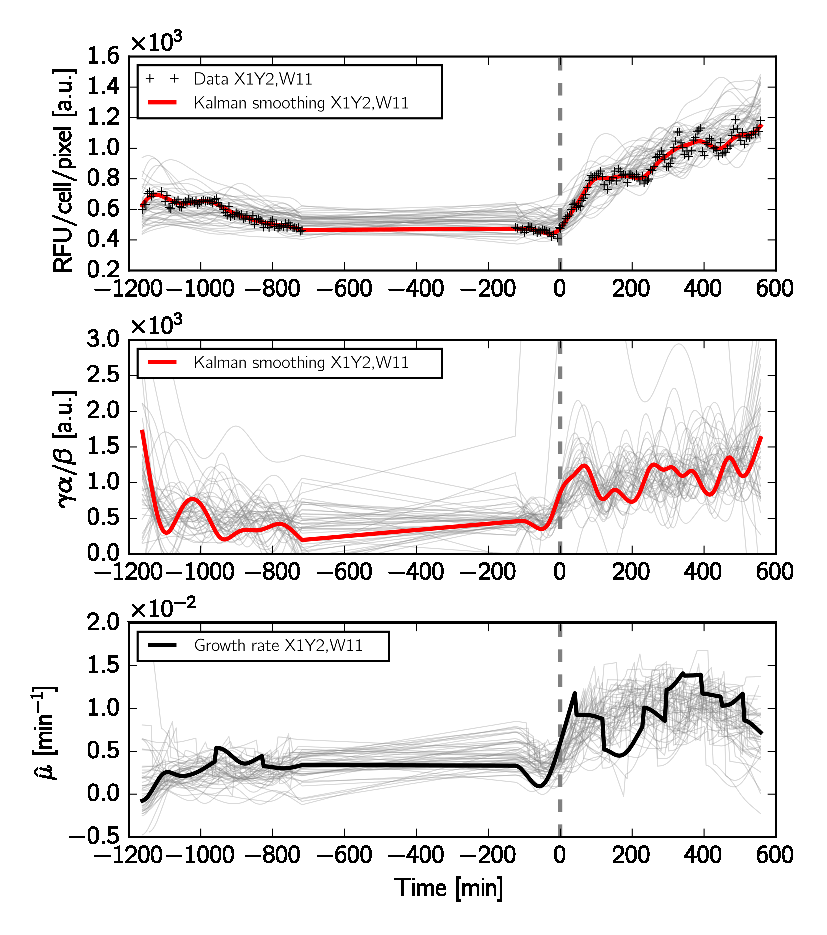
\includegraphics[scale=1]{./Fig/gene_activity}
\caption{
\textbf{Estimation of the resource allocation profile using Kalman smoothing based on the fluorescence density measurements and the estimated growth rates from Fig.~\ref{fig:growth_rate_estimation}.}
\textit{(A-B)} Gray lines represent the estimation of the fluorescence density (RFU/pixel) $F(\cdot)$ (in A) and the resource allocation profile $\gamma \alpha / \beta$ (in B) by the Kalman smoothing procedure for the 45 normal cells.
The solid red curves highlight the result for one particular cell, , located at the bottom of the well labelled "X3Y2, W2", while black crosses in the top graph are the data points for this cell.
The vertical dashed lines represent the time of the upshift from growth on acetate to growth on glucose.
The prior values for the parameters of the smoothing algorithm are exactly the same as those used for Fig.~\ref{fig:synthetic_upshift} and are reported in the Material and Methods~\ref{sec:meth_kalman}.
}
\label{fig:gene_activity}
\end{figure}

Nevertheless, when not focusing on the individual cells but looking at the statistics of the entire data set, some interesting patterns emerge. 
Fig.~\ref{fig:gene_activity_median} shows the median of the time-varying growth rate and resource allocation profile as well as the 25\%-75\% interquartile range. 
The use of these statistics gives a more robust view on the population level of the response of the cells to a nutrient upshift. 
When changing the carbon source from acetate to glucose, the growth rate increases to a value of around 0.011 min$^{-1}$, consistent with growth rates reported in the literature for the \textit{E. coli} strain used here~\cite{volkmer_condition-dependent_2011,izard_synthetic_2015}, before decreasing when the first cells start to die (Fig.~\ref{fig:gene_activity_median}\textit{C}).
In addition, the data show one period of an oscillation in the first 3~h after the upshift, conserved in each of the 25\%, 50\% and 75\% quartiles (Fig.~\ref{fig:gene_activity_median}\textit{B}).
The heatmap in Fig.~\ref{fig:gene_activity_heatmap} reveals that almost all of the normal cells show this oscillatory feature.
Moreover, the first peak is seen to be even more pronounced on the level of the individual cells, reflecting the fact that in the different cells it occurs at different times after the upshift and is therefore dampened out at the population level.
While the results of the microfluidic experiment presented here do not allow to confirm the occurrence of an on-off strategy for resource allocation after a nutrient upshift, the preliminary data are encouraging and prompt further investigation.

\begin{figure}[p]
\centering
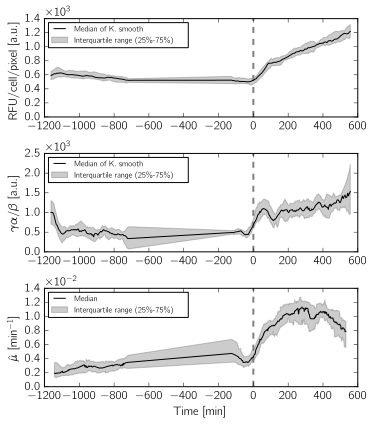
\includegraphics[scale=1]{./Fig/gene_activity_median}
\caption{
\textbf{Robust statistics for the estimation results presented in Fig.~\ref{fig:gene_activity}.}
Each graph shows the 25\% (lower gray curve), 50\% (solid black curve) and 75\% (upper gray curve) quartiles, computed at each time step for the signals reconstructed in Fig.~\ref{fig:gene_activity}.
The gray area represents the interquartile range.
Interestingly, while most oscillations in the resource allocation profile $\gamma \alpha (\cdot) / \beta$ cancel out at the population level, the first peak after the upshift is conserved.
}
\label{fig:gene_activity_median}
\end{figure}

\begin{figure}[tb]
\centering
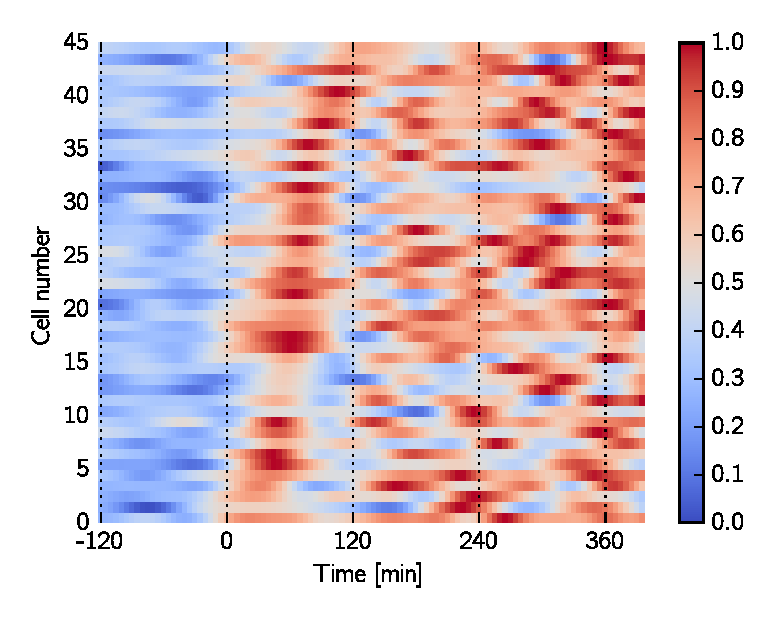
\includegraphics[scale=1]{./Fig/heatmap}
\caption{
\textbf{Global overview of all estimated resource allocation profiles presented in Fig.~\ref{fig:gene_activity}.}
The individual $\gamma \alpha (\cdot) / \beta$  curves have been normalized with respect to their maximum in the interval $[0, 400]$ and then ordered with respect to their maximum in the interval $[0, 120]$.
}
\label{fig:gene_activity_heatmap}
\end{figure}

\section{Discussion}
\label{sec:chap3_discussion}

As we showed in Chapter~\ref{chap:theory}, adopting a dynamical perspective might prove useful to unveil and understand the regulatory strategies employed by microorganisms.
The criterion of biomass maximization has allowed to account for steady-state empirical growth laws.
Interestingly, when the same criterion is applied to growth transitions, it predicts that microorganisms allocates their resources through bang-bang control of gene expression.
For the control of ribosome synthesis, the implementation of this optimal control scheme results in an on-off strategy, where a bacterial cell is either producing only ribosomes or not producing them at all during the adaptation to a new growth medium.
The ppGpp system, ubiquitous in bacteria and playing an important role in the control of ribosome synthesis in \textit{E. coli}, satisfies the requirements posed by the on-off strategy.
However, we currently lack experimental data to show that it actually functions in this manner, among other things because of the difficulties to produce well-controlled growth transitions on the single-cell level in the laboratory.
Can we set up appropriate experiments to measure the expression of ribosomes during a growth transitions?
Will the bacterial cells exhibit the on-off strategy that was shown to be close to optimal in Chapter~\ref{chap:theory}?

In this chapter, the above questions have been addressed by developing an experimental framework which allows the ribosome concentration to be quantified in individual \textit{E. coli} cells in real time.
Our main contribution consists in bringing together several experimental techniques developed in recent years.
First, inspired by the work of Bakshi \textit{et al.}~\cite{bakshi_superresolution_2012}, we constructed an \textit{E. coli} strain with fluorescent ribosomes.
In their paper, Bakshi \textit{et al} essentially used this fluorescent marker to localize ribosomes in the cytoplasm through superresolution microscopy.
While improving their design (Material and Methods~\ref{sec:methods_strain}), we used our strain for the purpose of quantifying ribosomal abundance in single cells.
Second, we employed the mother machine developed by Wang \textit{et al.}~\cite{wang_robust_2010}, originally developed to study long-term steady-state growth of \textit{E. coli}, to observe individual \textit{E. coli} cells growing in continuous culture by means of time-lapse fluorescence microscopy.
Here, the mother machine was used to establish well-controlled growth transitions, \textit{i.e.} from steady-state growth in minimal medium with acetate to steady-state growth in minimal medium with glucose.
By changing the medium source of the mother machine, we were able to observe how \textit{E. coli} cells adapt their growth rate and the expression of ribosomes.
Overall, through the combination of fluorescent labeling of a core component of the gene expression machinery and the use of a microfluidic device, we have opened the way to experimentally study growth laws in a dynamical context.

We applied this experimental set-up to the reconstruction of the resources allocation strategy employed by \textit{E. coli} during a nutrient upshift, with the aim to observe the bang-bang profile predicted in Chapter~\ref{chap:theory}.
We developed a Kalman smoothing procedure adapted to our question and showed how it can be implemented to reconstruct the internal state of a cell from time-lapse microscopy images.
Similar to hidden Markov chains, Kalman filtering and smoothing are powerful techniques for the reconstruction of unobserved signals from noisy measurements, and have had numerous applications in a variety of domains, though less in biology than in other fields.
We showed in this chapter that the Bayesian framework of Kalman smoothing can be exploited for growth rate reconstruction from a probabilistic prior defining the relation between mother and daughter cells.
We also developed another variant of Kalman smoothing for the reconstruction of the resource allocation variable $\alpha (\cdot)$ that is at the heart of the models of Chapter~\ref{chap:theory}.
Our work on synthetic data showed that, despite the challenge posed by the reconstruction of a discontinuous signal, the algorithm was capable of recovering an oscillatory pattern close to the expected on-off profile.
Unfortunately, its application to the real data did not allow an unambiguous conclusion to be drawn: while oscillations do occur, and a first peak between 0 and 120 min after the upshift is visible in almost all of the cells, it turned out to be far from straightforward to distinguish a real oscillatory pattern from artifacts of the data analysis and signal reconstruction methods.
Below we propose several improvements that will be addressed in future work.

Several experimental problems complicated the analysis of the data.
Sufficiently long steady-state measurements before and after the transition of interest are needed to provide a reliable estimation of the intensity and the nature of the experimental noise.
They are also critical to calibrate the parameters of the regularization method used for signal reconstruction.
Despite what was initially planned, we did not completely reach a new steady state after the transition.
Several causes are to blame.
First, the random stall of the motorization along the Z-axis of the microscope, which does not allow overnight measurements and occurred during the slow growth on acetate in the presented experiment.
Second, the massive death of bacteria starting after the transition on glucose.
Future work will focus on solving these issues.

The death of bacteria is particularly worrying.
During the construction of this strain, most people in the lab experienced contamination by an aggressive bacteriophage.
Unfortunately, the strain used in this study was not spared, and our frozen stocks were later tested positive for phage-induced lysis.
Interestingly, the lysis seems to depend strongly on the environmental conditions.
To our disarray, the massive death observed in this experiment suggests that a strong environmental upshift could trigger the lytic cycle of the phage.
While impeding any possible long-term measurement, the death of the bacteria is not our only worry.
Phages are machines that are extremely well optimized to divert cell resources to their own end, especially the activity of the gene expression machinery.
That could dramatically perturb the cell regulation of resource allocation, and so the conclusions of this study.
For this reason, future work will start by the reconstruction of a clean phage-free strain from scratch.

It is also possible to optimize the image analysis techniques used in this study.
We segmented the images using the most powerful and ubiquitous segmentation algorithm available: the human brain.
In other words, we manually selected the pixels representing the poles of a single bacteria per well on the fluorescence images, and used this information to arbitrarily define a rectangle around the cell of interest.
While this is far from satisfying, it may turn out to be difficult to improve upon this, as it seems that the first rule of image analysis is that every application is more or less unique.
Every algorithm has to make assumptions about the object it is trying to recognize.
For imaging of microbial cells, it could be the curvature at the poles, the size of the pixels, the homogeneity of the background, the homogeneity of intracellular fluorescence, ...
While some parameters can be tweaked, some assumptions are always hard-coded in the algorithm and reflect the philosophy used to address the identification problem.
Since the preliminary analysis reported here was completed, we started a collaboration with the authors of FluoBacTracker~\cite{fluobactracker} that focuses on adapting their software to our set-up in a near future.
It should provide a robust, automated way to identify and track the cells, enhancing the reproducibility of the analysis and increasing the number of cells available for computing population statistics.

The Kalman filtering algorithm that was later applied to these data can also be improved in many respects.
As described in the Results section, the algorithm is an instance of Bayesian inference and several parameters describing the expected input define a probabilistic prior.
In the work reported here, we chose these parameters through trial and error, or by calibrating the system on synthetic data whenever possible.
A better technique would be to choose these parameters by \textit{generalized cross-validation} (GCV)~\cite{golub_generalized_1979}, a procedure maximizing the predictive power of the reconstructed signal by reducing overfitting.
The use of GCV in our framework amounts to choosing the parameters of the Kalman smoother by optimizing predictions on a subset of the cells, then testing the performance on the remaining cells.
While the initial conditions did not seem to play a huge role in the final shape of the signal, the choice of the smoothing factor $\theta^2$ is critical and may strongly benefit from the proposed GCV extension.

The Kalman smoothing algorithm itself can also be further improved, notably by addressing the difficulty of estimating abrupt transitions.
As can be seen in Fig.~\ref{fig:synthetic_upshift}, the resource allocation profile $\gamma \alpha (\cdot) / \beta$ reconstructed from the synthetic data increases before the nutrient shift and this artifact also occurs when using the measured fluorescent densities (Fig.~\ref{fig:gene_activity_median}), the change in resource allocation preceding the nutrient upshift by several dozens of minutes.
While we know exactly when the change of medium occurs, this information is currently not used as a prior for the reconstruction.
The Kalman smoother can be improved by implementing time-varying parameters for the regularization method, so as to strongly penalize variations of the reconstructed signal at steady state and to release this constraint following the change in medium.

The improvements of the approach proposed in this section, which would help in reaching a conclusion about the existence of the on-off strategy, are not very complicated to realize.
Another improvement consists in taking into account the autofluorescence of the bacteria, which we assumed to be negligible, mostly because its proper estimation in a dynamical, single-cell context is complicated (Material and Methods~\ref{sec:cell_segmentation}).
A simple trick, however, could help in quantifying autofluorescence: mixing wild-type bacteria with bacteria having fluorescent ribosomes when loading the device.
This would allow some channels to be occupied by wild-type cells, in addition to the  channels in which the strain of interest is growing, and thus obtain a reliable estimation of the level of autofluorescence of the cells.
Notice though that the propertion between the two types of bacteria need to be carefully adjusted in order to preserve enough cells for the estimation of the resource allocation profile. 

%[I WOULD SKIP THIS FINAL PARAGRAPH OR REDUCE IT TO ONE PHRASE AND ADD IT TO THE DISCUSSION IN THE PARARAPH STARTING WITH "The Kalman smoothing algorithm..."]
%Something is also displeasing in the current implement of the Kalman smoothing method.
%As described in the main text, the Kalman smoothing procedure not only use previous measuments to estimate the state of the system, but also the next available measurements.
%This is a feature we totally lose in the estimation of the growth rate, because the discontinuities introduced by the cell divisions impede a global analysis of the time series.
%We partially solved the issue by using information about the mother cell at the beginning of the growth rate reconstruction of the daughter cells, but we did not find a way to implement it backward.
%There is probably a better way to deal with cell division in the analysis of microscopy data, and we are actively working on the matter.

\section{Material and Methods}

\subsection{Bacterial strain construction}
\label{sec:methods_strain}

To achieve dynamical quantification of ribosome abundance, we designed and constructed a strain containing a translational fusion of \textit{gfpmut2}~\cite{zaslaver_comprehensive_2006} to the C-terminus of \textit{rpsB} (the gene coding the ribosome subunit S2).
This design was inspired by the work of Bakshi \textit{et al}, who used a similar construction to assess the quantitative spatial distribution of ribosomes in living \textit{E.~coli}~\cite{bakshi_superresolution_2012}.

The transcription factor \textit{tsf} is under the control of the same promoter than \textit{rpsB}, and is located after the C-terminus.
In order to ensure that \textit{tsf} expression was not affected by our translation fusion on \textit{rpsB}, we used a double-selection procedure to get rid of every resistance gene that the construction might introduce.
This is something that was not done in the original construction from Bakshi \textit{et al}~\cite{bakshi_superresolution_2012}

A DNA fragment containing a double selection cassette was amplified with two long primers annealing respectively to the region just after the STOP codon at the C-terminus of \textit{rpsB}, and to the beginning of \textit{gfpmut2}.
The double-selection cassette contained a resistance gene to Kanamycin (positive selection) and a gene coding for the CcdB toxin under the control of the P\textsubscript{BAD} promoter (negative selection in presence of Arabinose).
This cassette is referred below as \textit{kan-P\textsubscript{BAD}-ccdB}.

Another DNA fragment containing \textit{gfpmut2}~\cite{zaslaver_comprehensive_2006} without ATG was amplified with long primers annealing respectively to the C-terminus of \ref{chap:theory}rpsB (just before the STOP codon), and the end of the \textit{kan-P\textsubscript{BAD}-ccdB} cassette.
The first primer also contained a 18-bp (base pair) linker that was chosen according to the method section of~\cite{bakshi_superresolution_2012}.

Both fragments (the \textit{gfpmut2} reporter and the \textit{kan-P\textsubscript{BAD}-ccdB} cassette) were assembled using Gibson assembly~\cite{gibson_enzymatic_2009}.
Both PCR products were quantified using NanoDrop and mixed in equimolar proportions with a commercial Gibson Assembly Master mix.
A final product of 2683 bp was obtained:
\begin{itemize}
\item *(50 bp) the C-terminus of \textit{rpsB} without the STOP codon 
\item (18 bp) a linker (see Supporting Information)
\item (714 bp) the \textit{gfpmut2} sequence without the initial ATG
\item (1851 bp) the \textit{kan-P\textsubscript{BAD}-ccdB} cassette
\item *(50 bp) the region directly after \textit{rpsB} in \textit{E.~coli}
\end{itemize}
Regions labeled with * are expected to anneal with the \textit{E.~coli} chromosome.
The complete sequence of this fragment, as well as all the primers used are available in the Supporting Information of this chapter.

This fragment was electroporated in a BW25113 background strain containing the pSIM5 plasmid with chloramphenicol resistance (lambda-red recombinaison).
A kanamycin-resistant colony was selected and verified to exhibit green fluorescence in a Tecan microplate reader.
A new 100-bp fragment containing 50 bp of the end of \textit{gfpmut2} and 50 bp of the region just after \textit{rpsB} was electroporated into this strain (sequence available in Supporting Information) to get rid of the \textit{kan-P\textsubscript{BAD}-ccdB} cassette.
An arabinose-resistant colony was selected and verified to be kanamycin-sensitive and to still exhibit green fluorescence.
Finally, the strain was grown overnight at 42$^\circ$C to get rid of the pSIM5 plasmid and a chloramphenicol-sensitive colony was selected.
The region after \textit{rpsB} was verified by sequencing (full sequence available in Supporting Information).

In parallel, the same protocol was used to construct \textit{mCherry} and \textit{cfp} variants of the same strain.
However, only the \textit{gfpmut2} and \textit{mCherry} versions were successfully obtained for reasons that were not investigated.
The full sequence of the final \textit{rpsB-mCherry} strain is available in Supporting Information.

The \textit{rpsB-gfpmut2} and \textit{rpsB-mCherry} strains were characterized on different media using a Tecan microplate reader.
They were showed to exhibit a wild-type growth rate and sufficient fluorescence level to allow quantification.
However, the \textit{rpsB-mCherry} strain exhibited strange fluorescence dynamics, especially during growth transitions, which made it unsuitable for our study.
Our effort were then concentrated on the \textit{rpsB-gfp} strain.
Data as well as information on the matter are available in Supporting Information.

\subsection{Growth conditions}
\label{sec:growth_condition}

Sterilization was performed by autoclaving for instruments and filtration for solutions (0.2 $\mu$m).
During cloning, bacteria were grown in 20-mL flasks filled with LB or spread on Petri dish with LA.
In all the experiments, we used M9 minimal medium~[citation to find] supplemented with trace elements, thiamine and a carbon source.
The full recipe is reproduced below.
Numbers in squared brackets are characteristics of the stock solution.
All stock solutions were stored at room temperature, except for FeSO$_4$~[30 g.L\textsuperscript{-1}] and Thiamine~[10 g.L\textsuperscript{-1}] that were stored respectively at -20$^\circ$C and 4$^\circ$C.
\begin{center}
\begin{tabular}{|l r|}
  \hline
  \multicolumn{2}{|c|}{\textbf{M9 medium (100 mL)}}\\
  \hline
  CaCl2 [1 mol.L\textsuperscript{-1}] & 10 $\mu$l\\
  MgSO$_4$ [1 mol.L\textsuperscript{-1}] & 200 $\mu$l\\
   5x Salts & 20 mL \\
  Traces elements & 90 $\mu$l \\
  FeSO$_4$ [30 g.L\textsuperscript{-1}] & 10 $\mu$l \\
  Thiamine [10 g.L\textsuperscript{-1}] & 50 $\mu$l \\
  Carbon source & at will \\
  H$_2$0 [18.2 M$\Omega$.cm] & to 100 mL \\
  \hline
\end{tabular}
\begin{tabular}{|l r|}
  \hline
  \multicolumn{2}{|c|}{\textbf{Traces elements (0.9 mL)}}\\
  \hline
  H$_2$0 [18.2 M$\Omega$.cm] & 200$\mu$l\\
  Na$_2$EDTA 2H$_2$O [150 g.L\textsuperscript{-1}] & 100$\mu$l\\
  ZnSO$_4$ 7H$_2$O [45 g.L\textsuperscript{-1}] & 100$\mu$l\\
  CoCl$_2$ 6H$_2$O [3 g.L\textsuperscript{-1}] & 100$\mu$l\\
  MnCl$_2$ 4H$_2$O [10 g.L\textsuperscript{-1}] & 100$\mu$l\\
  H$_3$BO$_3$ [10 g.L\textsuperscript{-1}] & 100$\mu$l\\
  Na$_2$MoO$_4$ 2H$_2$O [4 g.L\textsuperscript{-1}] & 100$\mu$l\\
  CuSO$_4$ 5H$_2$O [3 g.L\textsuperscript{-1}] & 100$\mu$l\\
  \hline
\end{tabular}
\begin{tabular}{|l r|}
    \hline
  \multicolumn{2}{|c|}{\textbf{5x Salts (100 mL)}}\\
  \hline
  Na$_2$HPO$_4$2H$_2$0 & 4.25 g \\
  KH$_2$HPO$_4$ & 1.5 mg \\
  NaCl & 0.25 g\\
  NH$_4$Cl& 0.5 g\\
  H$_2$0 [18.2 M$\Omega$.cm] & to 100 mL \\
  \hline
\end{tabular}
\end{center}

A large quantity of M9 was prepared several days before the experiment, and stored at 4$^\circ$C.
It contained all the necessary components except FeSO$_4$, thiamine, and carbon sources that were added the day the pre-culture were launched.
Except stated otherwise, the growth temperature was 37$^\circ$C.
M9 Acetate contains 0.2\% Acetate (in mass of C$_2$H$_3$O$_2$ per mass of solution), and M9 Glucose contains 0.2\% Glucose (in mass of D-(+)-Glucose per mass of solution).

At J-4, the glycerol stock containing the \textit{rpsB-gfp} strain was spread out on a Petri dish of LA, and incubated at 37$^\circ$C.
At J-3, an isolated colony was inseminated in 20 mL of M9 Acetate, and incubated in a cotton-plugged sterile flask (Fig.~\ref{fig:experiment_schema}).
Time of insemination was calculated to obtain a 0.3-0.4 cm\textsuperscript{-1} OD when starting the experiment, which correspond to a mid-exponential phase.

At J+0, the preculture was concentrated by centrifugation and back suspended into 5 mL of M9 Acetate supplemented with 50 mg.mL\textsuperscript{-1} BSA (passivation	buffer) for injection into the microfluidic device.
Channels were populated by diffusion until most of them were filled with cells ($\sim$1 hour).
Data acquisition started after a constant medium flow was successfully obtained ($\sim$1 hour, depending on the quality of the device).

\subsection{Microfluidic device}
\label{sec:microflu}

We used the mothermachine~\cite{wang_robust_2010}.
It consists of a series of growth wells (or channels), oriented at a 90$^\circ$ angle to a large central channel through which growth medium is passed at a constant flow.
The wideness of the wells is selected as to constrain the growth direction of the bacteria.
This design ensures that at least one cell per well (the deepest one) is preserved during the whole experiment, while the others incrementally escape into the central channel as divisions occur.
For the fabrication of the devices, we thoroughly followed the step described in the supporting information of~\cite{wang_robust_2010}.
We maintained a stock of chemically treated devices at room temperature (day 2 in workflow summary~\cite{wang_robust_2010}).
The day of the experiment, a single device was plasma cleaned, bond to a glass coverslip, and injected with bacteria (see section above).

The device was connected using 0.023" inner diameter polyethylene tubes to a waste and a sterile bottle containing 200 mL of growth medium, which was enough for several days of acquisition.
A microfluidic pump (Elvesys) containing an output flow sensor module was plugged to the medium bottle, and was applied a pressure up to 2 bars.
The output flow was set to 50 $\mu$L.min$^{-1}$.

For the imaging, the device was placed on a motorized inverted microscope (Zeiss Axiovert 200M) with a phase contrast objective lens (Zeiss PlanNeofluar, Ph3 100x/1.3), placed in a thermostated box at 37$^\circ$C.
In this setup, fluorescence illumination is provided by a mercury lamp (Osram, 1xHBO 103X/2) and visualization is performed with narrow-bandpass excitation and emission filters (Chroma, \#49002 ET-GFP and Chroma, \#49005 TR/DsRED ET).
The exposure time to the light source is externally controlled by mechanical shutters (Uniblitz-VS35).
Images are acquired with a 16-bit gray level CCDcamera cooled to -80$^\circ$C (Roper Scientific, Princeton Instruments PHOTOMAX 512) controlled by a custom-made software using Visual Basic and the Type libraries of the Winview software (Princeton Instruments).
Every 5 minutes, autofocus was numerically performed by maximizing the contrast of a region of interest, and a serie of acquisitions was made.
A total of 6 fields, each containing 15 wells was observed during the whole experiment.

\subsection{Cell segmentation}
\label{sec:cell_segmentation}

Raw data are in the form of 512x512-pixel 16-bit SPE images (proprietary format produced by the Princeton Instruments camera).
They were converted in 16-bit Tif images using the \textit{SPE} plugin of ImageJ~\cite{goto_open_2005}.
The rest of the analysis was performed using Python 3.5.2.
In particular, we used OpenCV~3.1.0-dev, Scikit-Image~0.12.3, Numpy~1.11.2 to manipulate the images.

The offset between consecutive images of a given field was evaluated using cross-correlation in the Fourier space~\cite{guizar-sicairos_efficient_2008} (see Scikit-Image documentation at \cite{skimage_cross-correlation}).
All the images for a field were then aligned on the first acquisition by simple affine translation.

The wells were isolated in individual images through a combination of manual pixel selection and automatic segmentation.
In particular, we selected the entrance of the two wells at the border of the image, and used this information along with the regularity of the microfluidic device to compute a mask that allowed to crop each well in its own image of size 100x21 pixels.
These sub-images were labeled $\left\{W0, W1, ..., W14\right\}$ depending on the position of the well on the original image, from left to right.

In this study, we performed a preliminary analysis on each well that focused on the deepest cell.
For each image, we manually selected two pixels representing the position of the poles of the cell of interest.
The distance between the two selected pixels was directly used as the bacteria length $L$ in pixels.
They were also used to compute a rectangular 6-pixel-wide mask around the cell (see Fig.~\ref{fig:data_acquisition}).
We then computed the RFU/pixel in this cell mask by summing each pixel and dividing by the mask size.

The camera noise and background was evaluated by taking a picture with a closed shutter at the end of the experiment.
Pixels in this picture were found to be Gaussian distributed with a mean of 1101.0 and a standard deviation of 10.788.
Correction for camera background was thus applied by removing 1101 to the computed RFU/pixel.

The background for autofluorescence of the bacteria and the medium was supposed negligible and was thus not corrected.
Indeed, the same device was used to image bacteria in stationary phase that do not produce any fluorescent protein.
They were entirely indistinguishable from the camera noise.
Not that this does not ensure that the autofluorescence is also negligible when the bacteria are actively growing.
Furthermore, its value could change with the medium of interest, and even be different at steady state and during growth transitions, which does not allow to estimate it independently.
In the section~\ref{sec:chap3_discussion}, we discuss possible improvements of the experimental set-up that would allow to dynamically co-estimate the autofluorescence with the ribosome abundance in a single experiment.

\subsection{Kalman smoothing}
\label{sec:meth_kalman}

The data about the length and the RFU/pixel of each bacteria were analyzed using Python~3.5.2.
In particular, we manipulated the data using Pandas~0.19.1, pykalman~0.9.5 and the curves submodule of wellfare~0.1.1.

Historical details about the Kalman smoothing procedure are reported in section~\ref{sec:res_kalman} of the main text.
We used the Additive Unscented Kalman Filter implementation of the pykalman python module.
This class is reported to be more stable and computationally efficient with non-linear problems featuring additive noises.

As described in section~\ref{sec:res_kalman}, the reconstruction of the growth rate was done on continuous portions of the length, \textit{i.e.} between two division events.
The full problem, as reported in Eq.~\ref{eq:full_mu_prob}, is reproduced below for clarity is:
\begin{eqnarray*}
\dot{V_\lambda}(t) &=& \mu (t) \cdot V_\lambda (t),\nonumber\\
\dot{\mu}(t) &=& v(t),\\
\dot{v}(t) &=& w(t),\nonumber
\end{eqnarray*}
with the measurement model:
\begin{equation*}
L(t_k) = V_\lambda(t_k) + \epsilon_k.
\end{equation*}
The parameters used as prior for the reconstruction of $\mu$ are reported below.
We used an observation variance of 9 pixels\textsuperscript{2} for the length $L$.
The transition variance $\theta^2$ (\textit{a.k.a.} the smoothing factor for $\mu$) is fixed at $10^{-8}$~min\textsuperscript{-6} during the whole time series.
Inheritance between mother and daughter cells is taken into account by systematically choosing an initial mean equal to the last estimated value for $\mu$, and to half the last estimated value for $V_\gamma$ (modeling the symmetrical division).
At the beginning of the experiment, were no mother cell are available, these values were fixed at 15~pixels for $V_\gamma$ and 0.004~min\textsuperscript{-1} for $\mu$.
The variances associated with these means are 16~pixels\textsuperscript{2} and $10^{-4}$~min\textsuperscript{-2}, respectively for $V_\gamma$ and $\mu$.
$v$ initial mean is always taken null, with an initial variance of $10^{-8}$~min\textsuperscript{-6}.
All the cross-covariances are set to 0 because the system variables are independent by construction.

For the reconstruction of gene activity, we only had to cope with the large gap in data acquisition between -720 and -150 min.
Reconstruction was then done independently on the continuous sections before and after this gap.
The full problem for the estimation of $u = \gamma \alpha / \beta$, as reported in Eq.~\ref{eq:full_u_prob}, is reproduced here for clarity:
\begin{eqnarray*}
\dot{r_\gamma}(t) &=& \hat{\mu} (t) \cdot u (t) - \hat{\mu} (t) \cdot r_\gamma (t), \nonumber\\
\dot{u}(t) &=& v(t),\\
\dot{v}(t) &=& w(t),\nonumber
\end{eqnarray*}
with the measurement model
\begin{equation*}
F(t_k) = r_\gamma (t_k) + \eta_k,\\
\end{equation*}
where $\hat{\mu}$ is the estimation of $\mu$ above.
In both case, we used as prior an observation variance of 800.4 RFU\textsuperscript{2} for $F$.
The transition variance $\theta^2$ (\textit{a.k.a.} the smoothing factor for $\gamma \alpha / \beta$) is fixed at $10^2$~RFU\textsuperscript{2}.min\textsuperscript{-4}.
The initial state means used are 600~RFU for $r_\gamma$ and 1000~RFU for $\gamma \alpha / \beta$.
The variances associated with these means are purposely large and fixed to 10\textsuperscript{6}~RFU\textsuperscript{2} for $r_\gamma$ and $\gamma \alpha / \beta$.
$v$ initial mean is always taken null, with an initial variance of $10^{-8}$~RFU.min\textsuperscript{-2}, imposing a null second derivative for the reconstructed signal $\gamma \alpha / \beta$.
Here again, all the cross-covariances are set to 0.

All the parameters cited in this section were chosen through trials and errors, and are as a consequence largely optimizable.
Possible improvements are discussed in section~\ref{sec:chap3_discussion}.

\section{Supporting Information for Chapter~3}

\subsection{S5 Text -- DNA sequences used for the strain construction}
\manuallabel{S5_Text}{S5~Text}

\subsubsection{Exhaustive list of the primers used...}

\paragraph{...for the \textit{gfpmut2} amplification.}

\begin{itemize}
\item[] 
\includegraphics[scale=1]{Fig/gfpmut2_L.png} \seqsplit{GTTCTCAGGATCTGGCTTCCCAGGCGGAAGAAAGCTTCGTAGAAGCTGAGCAGGAAAGGCGACAGGAGAGTAAAGGAGAAGAACTTTTCACTG}
(Length: 93)
\item[] 
\includegraphics[scale=1]{Fig/gfpmut2_R.png} \seqsplit{TGATGTTCTGGGGAATATAATTATTTGTATAGTTCATCCATGCC} (Length: 44)
\end{itemize}

\textbf{Rem.} The 50 first bases of the forward primer are supposed to anneal with the end of the \textit{rpsB} gene.
The 20 last bases of the reverse primer are supposed to anneal with the ccdB-end of the \textit{kan-P\textsubscript{BAD}-ccdB} cassette.


\paragraph{...for the \textit{mCherry} amplification}

\begin{itemize}
\item[] 
\includegraphics[scale=1]{Fig/mCherry_L.png} \seqsplit{GTTCTCAGGATCTGGCTTCCCAGGCGGAAGAAAGCTTCGTAGAAGCTGAGCAGGAAAGGCGACAGGAGACTAGCAAAAGATCCAAGGG}
(Length: 88)
\item[] 
\includegraphics[scale=1]{Fig/mCherry_R.png} \seqsplit{TGATGTTCTGGGGAATATAATTATTTGTACAGCTCATCCATG} (Length: 42)
\end{itemize}

\textbf{Rem.} The 50 first bases of the forward primer are supposed to anneal with the end of the \textit{rpsB} gene.
The 20 last bases of the reverse primer are supposed to anneal with the ccdB-end of the \textit{kan-P\textsubscript{BAD}-ccdB} cassette.

\paragraph{...for the cassette amplification}

\begin{itemize}
\item[] 
\includegraphics[scale=1]{Fig/cassette_L} \seqsplit{TGGATGAACTATACAAATAATTATATTCCCCAGAACATCAGG}
(Length: 42, used to assemble with gfp)
\item[] 
\includegraphics[scale=1]{Fig/cassette_L} \seqsplit{TGGATGAGCTGTACAAATAATTATATTCCCCAGAACATCAG}
(Length: 41, used to assemble with mCherry)
\item[] 
\includegraphics[scale=1]{Fig/cassette_R} \seqsplit{GAGCTTGCCGCCTTTCTGCAACTCGAACTATTTTGGGGGAGTTATCAAGCTTAGAAGAACTCGTCAAGAAGG}
(Length: 72, used for both)
\end{itemize}

\textbf{Rem.} The 20 first bases of the first forward primer are supposed to anneal with the end of the \textit{gfpmut2} gene.
The 20 first bases of the second forward primer are supposed to anneal with the end of the \textit{mCherry} gene.
The 50 last bases of the reverse primer are supposed to anneal with the region after \textit{rpsB} on the \textit{E.~coli} BW25113 chromosome.


\paragraph{...for the whole insert amplification}

\begin{itemize}
\item[] 
\includegraphics[scale=1]{Fig/overlap_L} \seqsplit{GTTCTCAGGATCTGGCTTCCCAGG}
(Length: 24)
\item[] 
\includegraphics[scale=1]{Fig/overlap_R} \seqsplit{GAGCTTGCCGCCTTTCTGCA} (Length: 20)
\end{itemize}

\paragraph{...for the cassette elimination}

\begin{itemize}
\item[\textbf{\textit{rpsB-gfpmut2}}] \seqsplit{TTGTAACAGCTGCTGGGATTACACATGGCATGGATGAACTATACAAATAAGCTTGATAACTCCCCCAAAATAGTTCGAGTTGCAGAAAGGCGGCAAGCTC}
(Length: 100)
\item[\textbf{\textit{rpsB-mCherry}}] \seqsplit{GCGCGGAGGGTCGTCATTCTACCGGTGGCATGGATGAGCTGTACAAATAAGCTTGATAACTCCCCCAAAATAGTTCGAGTTGCAGAAAGGCGGCAAGCTC}
(Length: 100)
\end{itemize}


\paragraph{...for the sequencing of the final strain}

\begin{itemize}
\item[] 
\includegraphics[scale=1]{Fig/sequencing_L} \seqsplit{CGTCTGAAAGACCTGGAAAC}
(Length: 20)
\item[] 
\includegraphics[scale=1]{Fig/sequencing_R} \seqsplit{AAACGTGTACTACCTGGTCTATAAGG} (Length: 26)
\end{itemize}

\subsubsection{Full annotated sequences of the inserts}

The following pages contain the full sequences of the \textit{gfpmut2-cassette} and \textit{mCherry-cassette} constructions, inserted on the \textit{E.~coli} BW25113 chromosome at the region after the \textit{rpsB} gene.
The primers annealing positions are indicated using the same color code as in the description of the primers above.
The primers reported in the original publication of Bakshi \textit{et al}~\cite{bakshi_superresolution_2012} are indicated for information.

\includepdf[pages={1-7}]{./Fig/gfp-mut2-cassette-after-rpsB-gene-sequence.pdf}
\includepdf[pages={1-6}]{./Fig/mcherry-cassette-after-rpsB-gene-sequence.pdf}

\subsubsection{Sequencing of the final strains}

The strains were constructed using the protocol described in Material and Methods~\ref{sec:methods_strain}.
Regions at the end of the \textit{rpsB} gene were amplified, and sent for sequencing.
Alignments of the results showed they exhibit the expected sequences (except for a couple of single-base mutations).
The raw results of the sequencing are reproduced below.

\paragraph{Final sequences of the \textit{rpsB-gfpmut2} strain (region after \textit{rpsB})}

\begin{small}
\begin{itemize}
\item[] 
\includegraphics[scale=1]{Fig/sequencing_L} \seqsplit{AGAAAGAAGCGCTGTATGCGCACTCGTGAGCTGGAGAAACTGGAAAACAGCCTGGGCGGTATCAAAGACATGGGCGGTCTGCCGGACGCTCTGTTTGTAATCGATGCTGACCACGAACACATTGCTATCAAAGAAGCAAACAACCTGGGTATTCCGGTATTTGCTATCGTTGATACCAACTCTGATCCGGACGGTGTTGACTTCGTTATCCCGGGTAACGACGACGCAATCCGTGCTGTGACCCTGTACCTGGGCGCTGTTGCTGCAACCGTACGTGAAGGCCGTTCTCAGGATCTGGCTTCCCAGGCGGAAGAAAGCTTCGTAGAAGCTGAGCAGGAAAGGCGACAGGAGCGTAAAGGAGAAGAACTTTTCACTGGAGTTGTTCCAATTCTTGTTGAATTAGATGGTGATGTTAATGGGCACAAATTTTCTGTCAGTGGAGAGGGTGAAGGTGATGCAACATA}
\item[] 
\includegraphics[scale=1]{Fig/sequencing_R} \seqsplit{CGCCGCAGATGCGTTATCTTCGCTCGCTCATCCCGGTCACTTACTGATGTAAGCTCCCGGGAATTCTCGAGCTTGCCGCCTTTCTGCAACTCGAACTATTTTGGGGGAGTTATCAAGCTTATTTGTATAGTTCATCCATGCCATGTGTAATCCCAGCAGCTGTTACAAACTCAAGAAGGACCATGTGGTCTCTCTTTTCGTTGGGATCTTTCGAAAGGGCAGATTGTGTGGACAGGTAATGGTTGTCTGGTAAAAGGACAGGGCCATCGCCAATTGGAGTATTTTGTTGATAATGGTCTGCTAGTTGAACGCTTCCATCTTCAATGTTGTGTCTAATTTTGAAGTTAACTTTGATTCCATTCTTTTGTTTGTCTGCCATGATGTATACATTGTGTGAGTTATAGTTGTATTCCAATTTGTGTCCAAGAATGTTTCCATCTTCTTTAAAATCAATACCTTTTAACTCGATTCTATTAACAAGGGTATCACCTTCAAACTTGACTTCAGCACGTGTCTTGTAGTTCCCGTCATCTTTGAAAAATATAGTTCTTTCCTGTACATAAACCTTCGGGCATGGCACTCTTGAAAAAGTCATGCTGTTTCATATGATCTGGGTATCTCGCAAAGCATTGAAGACCATACGCGAAAAGTAGTGACAAGTGTTGGCCATGGAACAGGTAGTTTTCCAGTAGTGCAAATAAATTTAAGGGTAAAGTTTTCCGTATGTTGCATCACCTTCACCCTCTCCACTGACAGAAAAATTTGTGCCCATTTAACATCACCATCTAATTCAACAAGAATTGGAAACAACTCCAGTGAAAGT} 
\end{itemize}
\end{small}

\newpage
\paragraph{Final sequences of the \textit{rpsB-mCherry} strain (region after \textit{rpsB})}

\begin{small}
\begin{itemize}
\item[] 
\includegraphics[scale=1]{Fig/sequencing_L}
\seqsplit{TTTCGACAGCTGACCAAGAAGAAGCGCTGATGCGCACTCGTGAGCTGGAGAAACTGGAAA
ACAGCCTGGGCGGTATCAAAGACATGGGCGGTCTGCCGGACGCTCTGTTTGTAATCGATG
CTGACCACGAACACATTGCTATCAAAGAAGCAAACAACCTGGGTATTCCGGTATTTGCTA
TCGTTGATACCAACTCTGATCCGGACGGTGTTGACTTCGTTATCCCGGGTAACGACGACG
CAATCCGTGCTGTGACCCTGTACCTGGGCGCTGTTGCTGCAACCGTACGTGAAGGCCGTT
CTCAGGATCTGGCTTCCCAGGCGGAAGAAAGCTTCGTAGAAGCTGAGCAGGAAAGGCGAC
AGGAGACTAGCAAAAGATCCAAGGGCGAGGAGGATAACATGGCTATCATTAAAGAGTTCA
TGCGCTTCAAAGTTCACATGGAGGGTTCTGTTAACGGTCACGAGTTCGAGATCGAAGGCG
AAGGCGAGGGCCGTCCGTATGAAGGCACCCAGACCGCCAAACTGAAAGTGACTAAAGGCG
GCCCGCTGCCTTTTGCGTGGGACATCCTGAGCCCGCAATTTATGTACGGTTCTAAAGCGT
ATGTTAAACACCCAGCGGATATCCCGGACTATCTGAAGCTGTCTTTTCCGGAAGGTTTCA
AGTGGGAACGCGTAATGAATTTTGAAGATGGTGGTGTCGTGACCGTCACTCAGGACTCCT
CCCTGCAAGATGGCGAGTTCATCTATAAAGTTAAACTGCGTGGTACTAATTTTCCATCTG
ATGGCCCGGTGATGCAGAAAAAGACGATGGGTTGGGAGGCGTCTAGCGAACGCATGTATC
CGGAAGATGGTGCGCTGAAAGGCGAAATTAAACAGCGCCTGAAACTGAAAGATGGCGG}
\item[] 
\includegraphics[scale=1]{Fig/sequencing_R}
\seqsplit{TTCGCGCCGCAGATGCGTTATCTTCGCTCGCTCATCCCGGTCACTTACTGATGTAAGCTC
CCGGGAATTCTCGAGCTTGCCGCCTTTCTGCAACTCGAACTATTTTGGGGGAGTTATCAA
GCTTATTTGTACAGCTCATCCATGCCACCGGTAGAATGACGACCCTCCGCGCGCTCATAT
TGCTCTACGATCGTATAATCTTCATTATGAGAGGTGATGTCCAGTTTAATATTCACATTG
TACGCGCCAGGCAGCTGCACAGGTTTCTTGGCTTTGTACGTGGTTTTCACTTCAGCGTCA
TAATGGCCGCCATCTTTCAGTTTCAGGCGCTGTTTAATTTCGCCTTTCAGCGCACCATCT
TCCGGATACATGCGTTCGCTAGACGCCTCCCAACCCATCGTCTTTTTCTGCATCACCGGG
CCATCAGATGGAAAATTAGTACCACGCAGTTTAACTTTATAGATGAACTCGCCATCTTGC
AGGGAGGAGTCCTGAGTGACGGTCACGACACCACCATCTTCAAAATTCATTACGCGTTCC
CACTTGAAACCTTCCGGAAAAGACAGCTTCAGATAGTCCGGGATATCCGCTGGGTGTTTA
ACATACGCTTTAGAACCGTACATAAATTGCGGGCTCAGGATGTCCCACGCAAAAGGCAGC
GGGCCGCCTTTAGTCACTTTCAGTTTGGCGGTCTGGGTGCCTTCATACGGACGGCCCTCG
CCTTCGCCTTCGATCTCGAACTCGTGACCGTTAACAGAACCCTCCATGTGAACTTTGAAG
CGCATGAACTCTTTAATGATAGCCATGTTATCCTCCTCGCCCTTGGAT} 
\end{itemize}
\end{small}

\clearpage
\subsection{S6 Text -- Strain validation in batch growing conditions}
\manuallabel{S6_Text}{S6~Text}

(signal-to-noise ratio, growth rate not hampered in microplate reader)
Difference between mCherry and GFP (mCherry not good because so and so, GFP was chosen)

Two type of strains were obtained

Before being used in the microscopy experiments, the strain characteristics were validated by 

\begin{figure}[p]
\centering
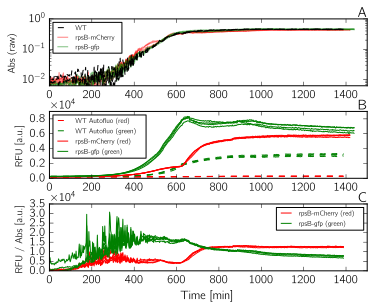
\includegraphics[scale=1]{./Fig/suppinfo_caract}
\caption{
\textbf{Growth curves in M9~0.2\% glucose for the \textit{rpsB-gfp} and \textit{rpsB-mCherry} strains.}
Growth and measurements were performed in a 96-well microplate placed in a Tecan infinite 200 pro reader thermostated at 37$^\circ$C.
We monitored 4 wells inseminated with the WT strain, the \textit{rpsB-gfp} strain, and the \textit{rpsB-mCherry} strain, for a total of 12 wells each containing 150~$\mu$L of growth medium.
Curves were shifted in time to correct for pipetting variability in the insemination process (-50 min for WT, and -20 min for \textit{rpsB-mCherry}).
\textit{(A)}~The light absorbance as measured by the Tecan microplate reader, corrected for background by removing well containing clean M9.
The superposition of the curves indicates similar growth rates between the WT and the modified strains.
\textit{(B)}~The fluorescence measured in the wells, expressed in Relative Fluorescence Units (RFU).
Green fluorescence (485nm excitation, 535nm reception) is measured for the WT (dashed lines) and the \textit{rpsB-gfp} (solid lines) strains.
Red fluorescence (560nm excitation, 635nm reception) is measured for the WT (dashed lines) and the \textit{rpsB-mCherry} (solid lines) strains.
As can be seen, fluorescence levels of the modified strains (solid lines) are far above the autofluorescence measured on the WT strain.
\textit{(C)}~The ratio of fluorescence over absorbance, a proxy for the fluorescence concentration in the cells.
Autofluorescence background was corrected by removing the autofluorescence measured on the WT wells.
We observe a strange increase in fluorescence concentration for the \textit{rpsB-mCherry} strain at stationary phase, something that is not visible on the \textit{rpsB-gfp} strain.
Before each measurement cycle, the following procedure was applied: shaking (Orbital 6mm) for 30~s, shaking (Linear 6mm) for 30~s, waiting for 5~s.
}
\label{fig:suppinfo_caract}
\end{figure}

\clearpage
\subsection{S7 Text -- Noise estimation in the microscopy experiment}
\manuallabel{S7_Text}{S7~Text}

We estimated the noise in the RFU/pixel/cell by using the data points just before upshift (Fig.~\ref{fig:noise_poi}).
Since they have been growing for 20~h on acetate in the microfluidic device, bacteria are assumed in balanced growth in this region of $\sim$2~hours (roughly 23-24 points depending on the well of interest).
For this reason, ribosome concentration, and so fluorescence concentration, are expected constant.
Fig.~\ref{fig:noise_poi} represents the distribution of points in this region for a particular cell, that can be approximated by a Gaussian distribution.

\begin{figure}[p]
\centering
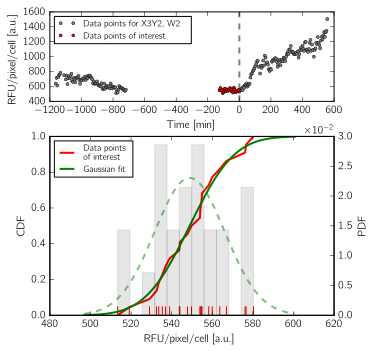
\includegraphics[scale=1]{./Fig/noise_poi}
\caption{
\textbf{Point of interest for the noise estimation.}
\textit{(Top graph)} RFU/pixel/cell data points for the cell at the bottom of the well labeled X3Y2,W2.
Noise estimation was performed on the points just before the upshift (red points), were the bacteria is assumed to grow at steady state.
\textit{(Bottom graph)} Cumulative density function (CDF, in red) and probability density function (CDF, in gray) of the points highlighted in red on the top graph.
They are visually compared with CDF (solid green line) and PDF (dashed green line) of a Gaussian fit with mean 548.88 and standard deviation 17.316.
}
\label{fig:noise_poi}
\end{figure}

Interestingly, as can be seen in Fig.~\ref{fig:noise_distrib_mean_std}, the mean and standard deviation of the distribution vary from cell to cell in a slightly correlated manner (Pearson R\textsuperscript{2}: $0.3213$, p-value: $4.923\cdot10^{-5}$).
We did not investigate if this heterogeneity between cells is the result of true biological variations or a bias due to the microfluidic device.
By looking at the points of Fig.~\ref{fig:noise_distrib_mean_std}, there are however no strong correlation of the mean and standard deviation with the acquisition field (XY), or the position of the well on the image (W).

\begin{figure}[tb]
\centering
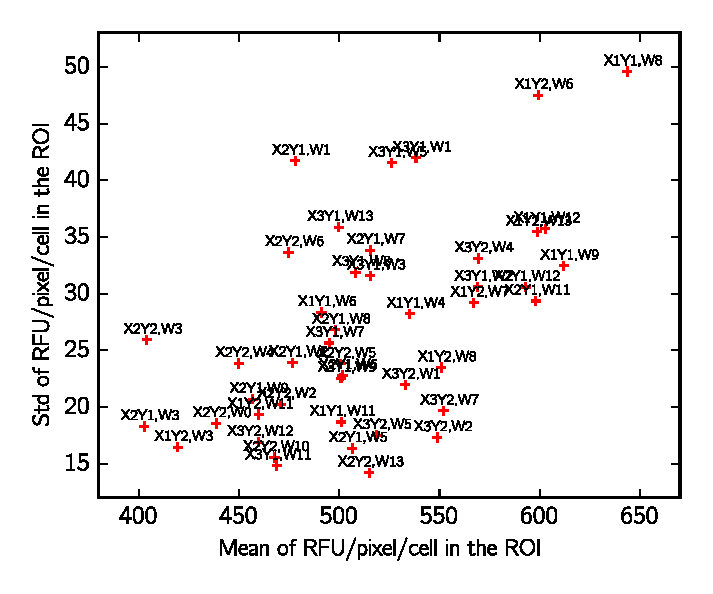
\includegraphics[scale=1]{./Fig/noise_distrib_mean_std}
\caption{
\textbf{Distribution of the means and standard deviations in the region of interest for the normal cells.}
The empirical mean and standard deviation were evaluated in the region before the upshift (red points on Fig.~\ref{fig:noise_poi}) for each of the 45 normal cells.
They appear to be slightly correlated (Pearson R\textsuperscript{2}: $0.3213$, p-value: $4.923\cdot10^{-5}$) which could indicate a multiplicative instead of an additive noise.
}
\label{fig:noise_distrib_mean_std}
\end{figure}

Noise characteristics were computed by normalizing and aggregating data for the 45 normal cells presented in Fig.~\ref{fig:noise_distrib_mean_std}.
Two scenarii were considered.
First, the noise model can be considered additive, which means we have the measurement model presented in Section~\ref{sec:estim_gr_ra}:
\begin{equation}
F(t_k) = \gamma r (t_k) + \eta_k,\\
\end{equation}
were $F(t_k)$ is the fluorescence measured at the time step $t_k$, $r (t_k)$ is the true ribosomal concentration at this time step, $\gamma$ is an unknown factor, and $\eta_k$ is the measurement noise.
In this scenario, for a time independent ribosome concentration $r$ (steady state), the ribosome concentration is constant and equal to its mean on the interval of interest (noted $m_k(\cdot)$).
Given that
\begin{equation}
m_k (F) = m_k (\gamma r) + m_k(\eta_k) = \gamma m_k (r),\\
\end{equation}
the noise residues are given by
\begin{equation}
\eta_k = F(t_k) - m_k (F). \label{eq:noise_add}
\end{equation}
In other words, we can normalize the data points of each cell by removing their mean in order to aggregate the noise residues and get an estimation of the noise level (Fig.~\ref{fig:noise_estim_add_mul}, top panel).

Secondly, the noise model can be considered multiplicative.
The noise model is than different than presented in Section~\ref{sec:estim_gr_ra}, and can be re-written:
\begin{equation}
F(t_k) = \gamma r (t_k) \cdot (1 + \lambda_k),
\end{equation}
were $\gamma r (t_k) \cdot \lambda_k$ is the measurement noise, proportional to the value measured.
In that scenario, with the same notations as above, the noise $\lambda_k$ is given by
\begin{equation}
\lambda_k = \frac{F(t_k)}{m_k (F)} - 1, \label{eq:noise_mul}
\end{equation}
which means we can normalize data points from different cells by dividing by the mean and removing 1 (Fig.~\ref{fig:noise_estim_add_mul}, bottom panel).

Both models were considered and are represented in Fig.~\ref{fig:noise_estim_add_mul}.
Despite the correlation identified in Fig.~\ref{fig:noise_distrib_mean_std}, the means of the residues in both models are very close to zero, and the distributions are well approximated by a Gaussian distribution.
For this reason, we decided in the main analysis to stick with an additive noise, the main reason being that the implementation used for the Kalman smoothing procedure are faster and more stable with an additive noise model.
We thus assumed an additive white Gaussian noise with mean 0 and standard deviation 28.29 for the simulation of the synthetic data and the signal reconstruction through the Kalman smoothing procedure.
As discussed in Section~\ref{sec:chap3_discussion}, the only way to decisively choose a noise model over the other would have been to obtain two different steady-state growths for the each cell.
Unfortunately, the presented time series were not long enough to obtain a new steady state on glucose, something that will be corrected in future instances of the experiment.

\begin{figure}[p]
\centering
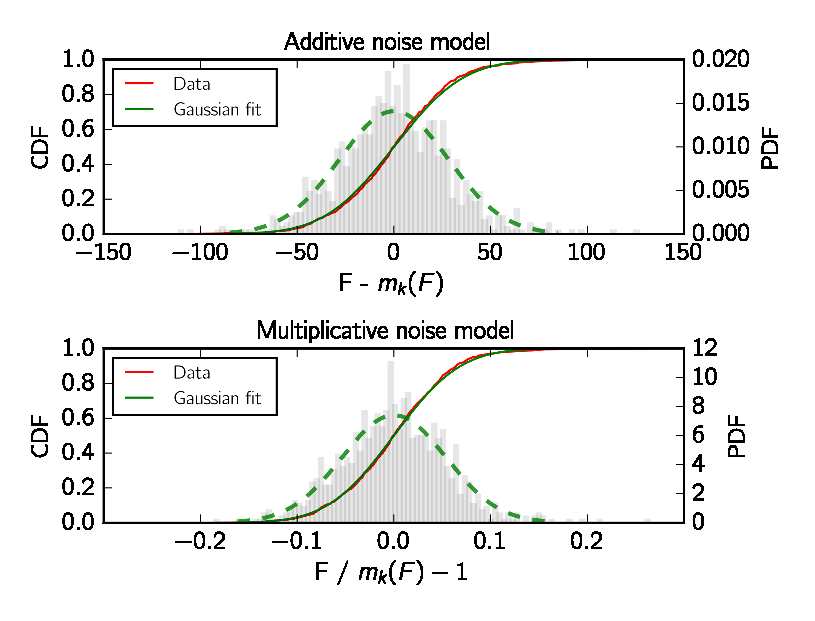
\includegraphics[scale=1]{./Fig/noise_estim_add_mul}
\caption{
\textbf{Distribution of the noise residues after normalization and aggregation for the 45 normal cells.}
Two noise models were considered for the normalization: either the temporal mean $m_k (\cdot)$ was removed from the measurements independently for each cell (additive noise model in Eq.~\ref{eq:noise_add}), or $1$ was removed from the ratio of the measurements with the temporal mean $m_k (\cdot)$ (multiplicative noise model in Eq.~\ref{eq:noise_mul}).
For the additive noise model, the fitted Gaussian distribution as a mean of $1.256\cdot 10^{-15}$ and a standard deviation of 28.29.
For the multiplicative noise model, the fitted Gaussian distribution as a mean of $2.666\cdot 10^{-18}$ and a standard deviation of 0.05383.
}
\label{fig:noise_estim_add_mul}
\end{figure}

\clearpage
\subsection{S8 Text -- Examples of complete analysis for 5 normal cells}
\manuallabel{S8_Text}{S8~Text}

To help the reader get a better idea on the analysis, we display below the complete reconstructions for 5 cells.
In Figs~\ref{fig:cell1}-\ref{fig:cell5}, the image on the left is the last image analyzed for the corresponding well.
The bacteria either at the top or the bottom (depending on the orientation in the device) was manually segmented by selecting two pixels at the poles on the fluorescence images (red cross).
A 6-pixel-wide rectangular mask was computed for each image, resulting in the masked image on the right.
In each of the graphs, the black and green points represents data points, while the red solid lines are the results of the signal reconstruction \textit{via} the Kalman smoothing procedure, the parameters of which are described in Material and Methods~\ref{sec:meth_kalman} and Figs~\ref{fig:growth_rate_estimation} and \ref{fig:gene_activity}.
Specific comments on each cell are given in the caption of Figs~\ref{fig:cell1}-\ref{fig:cell5}.

\begin{figure}[p]
\centering
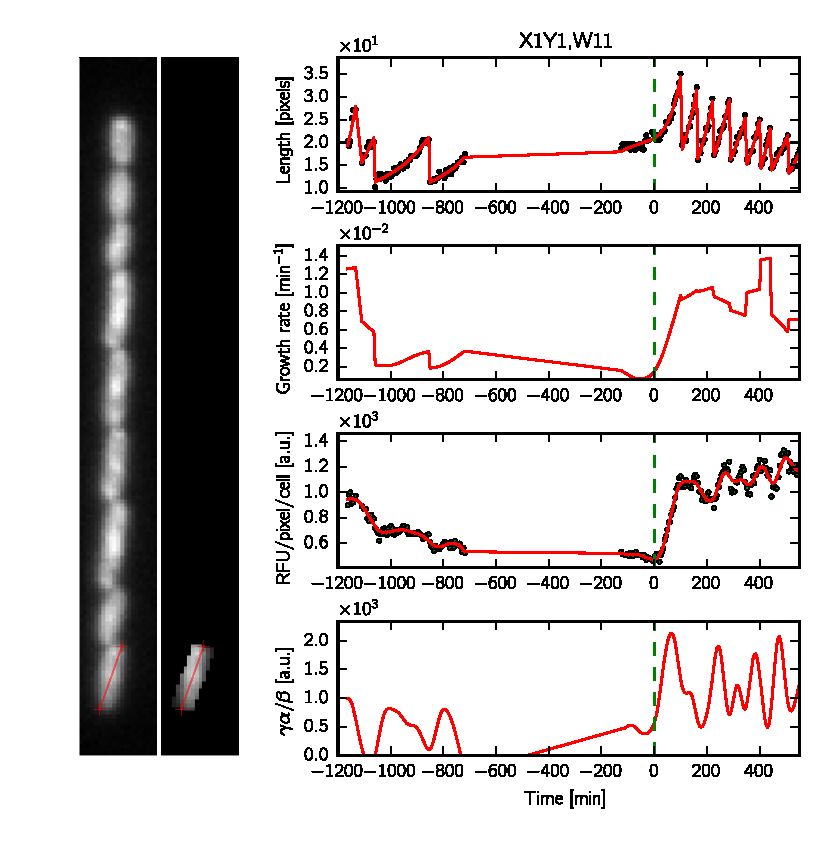
\includegraphics[scale=1]{./Fig/cell1}
\caption{
\textbf{Complete analysis for the cell located at the bottom of the well labelled "X1Y1, W11".}
(Figure description available in the introduction of \ref{S8_Text}.)\newline
Growth rate and resource allocation are particularly unstable at the beginning of the experiment, but seems to have stabilized before the upshift.
Oscillations in the RFU/pixel/cell signal are clearly visible, which results in oscillations in the resource allocation signal reconstruction, even though the smoothing factor seems a little too high for this particular cell.
}
\label{fig:cell1}
\end{figure}

\begin{figure}[p]
\centering
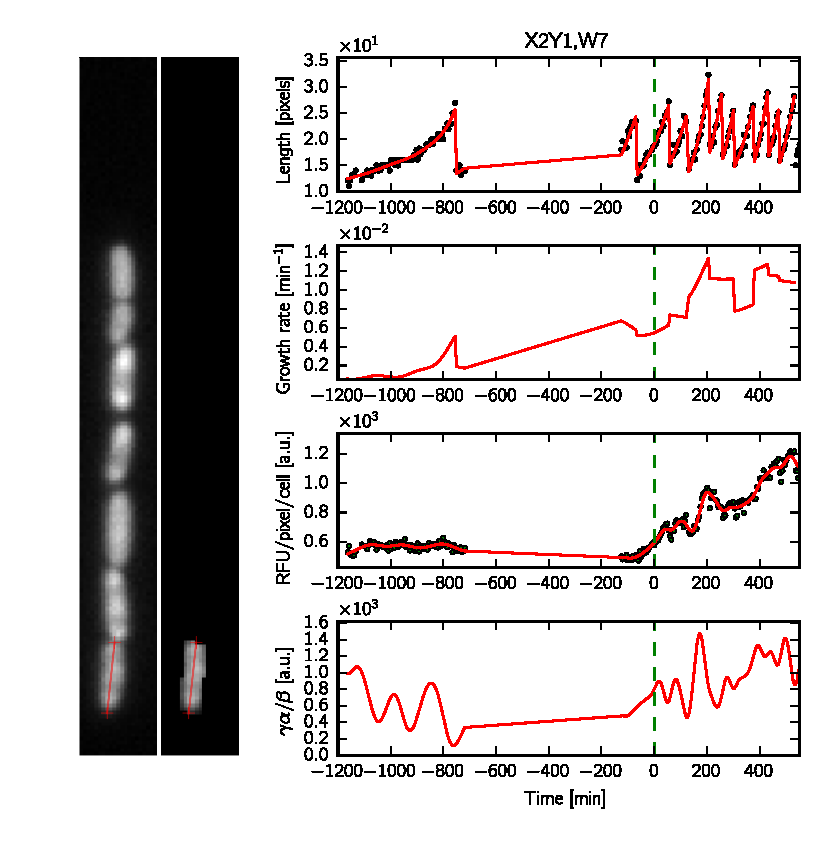
\includegraphics[scale=1]{./Fig/cell2}
\caption{
\textbf{Complete analysis for the cell located at the bottom of the well labelled "X2Y1, W7".}
(Figure description available in the introduction of \ref{S8_Text}.)\newline
Here, the resource is unstable at the beginning of the experiment despite the apparent regularity of the RFU/pixel/cell.
This could indicate a smoothing factor that is too low for this particular cell.
}
\label{fig:cell2}
\end{figure}

\begin{figure}[p]
\centering
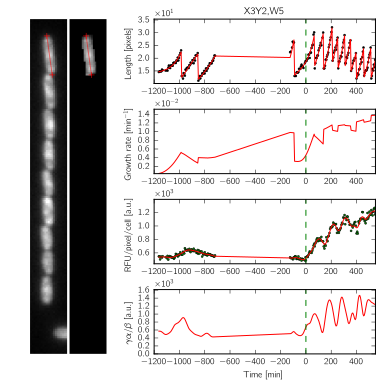
\includegraphics[scale=1]{./Fig/cell3}
\caption{
\textbf{Complete analysis for the cell located at the bottom of the well labelled "X3Y2, W5".}
(Figure description available in the introduction of \ref{S8_Text}.)\newline
We see for this cell that the reconstruction of the growth rate on the acetate medium (before 0) is affected by the huge gap in the acquisition, the increase before -150~min clearly being an artifact.
However, because the Kalman smoothing procedure we used allows for flexibility between the mother and the daughter cell, we quickly recover a more realistic growth rate before the upshift.
Despite an instability at the beginning of the experiment, the resource allocation reconstruction exhibits a remarkable stability during growth on the acetate medium, followed by oscillations after the upshift on glucose (also visible directly on the RFU/pixel/cell data).
}
\label{fig:cell3}
\end{figure}

\begin{figure}[p]
\centering
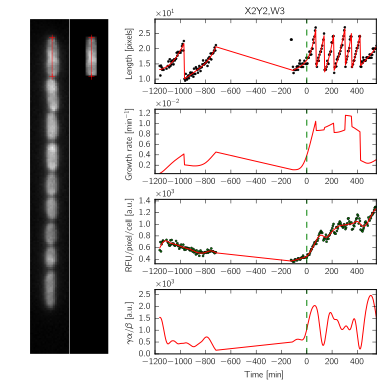
\includegraphics[scale=1]{./Fig/cell4}
\caption{
\textbf{Complete analysis for the cell located at the bottom of the well labelled "X2Y2, W3".}
(Figure description available in the introduction of \ref{S8_Text}.)\newline
The reconstruction on this cell is a good instance of what we aimed to obtain: the growth rate is stable on acetate, than quickly increases after the upshift on glucose.
The resource allocation is stable on a acetate (indicating a steady state) than starts to oscillate after the upshift on glucose.
}
\label{fig:cell4}
\end{figure}

\begin{figure}[p]
\centering
\includegraphics[scale=1]{./Fig/cell5}
\caption{
\textbf{Complete analysis for the cell located at the bottom of the well labelled "X1Y2, W6".}
(Figure description available in the introduction of \ref{S8_Text}.)\newline
The results on this cell are particularly terrible: we do not seem to get a good steady state on acetate since the reconstructed resource allocation appears either negative or oscillating.
The oscillations after the upshift are thus very hard to interpret.
}
\label{fig:cell5}
\end{figure}

\clearpage
\subsection{S2 Figure -- Cell categories identified in the microscopy analysis}
\manuallabel{S2_Figure}{S2~Fig}

\begin{figure}[h]
\centering
\includegraphics[scale=1]{./Fig/subcat_cells}
\caption{
\textbf{Cell categories identified in the microscopy analysis.}
As stated in Section~\ref{sec:estim_gr_ra}, the reconstruction of the growth rate for the 68 available cells motivated their classification in three categories: the dying cells (lowest graphs) stop growing, pausing cells (middle graph) present growth rate oscillations, and normal cells (highest graph) does not present any of the above}
\label{fig:subcat_cells}
\end{figure}

\clearpage
\subsection{S3 Figure -- Robust statistics for the cell categories}
\manuallabel{S3_Figure}{S3~Fig}

\begin{figure}[h]
\centering
\includegraphics[scale=1]{./Fig/subcat_median}
\caption{
\textbf{Robust statistics for the cell categories identified in the microscopy analysis.}
Each graph shows the 25\% (lower gray curve), 50\% (solid black curve) and 75\% (upper gray curve) quartiles, computed at each time step for the growth rate presented in~\ref{S2_Figure}.
The gray area represents the interquartile range.
}
\label{fig:subcat_median}
\end{figure}

\chapter{Discussion}
\label{chap:discussion}

\textit{"Apples fall onto the Earth because natural selection eliminated apples falling towards the sky."} -- @tomroud~\cite{tomroud_tom_2016}, original source unknown.

\selectlanguage{french}
\section*{Résumé en français}

Dans cette section... (env. 1 page)
\selectlanguage{english}

\begin{center}
\noindent\rule{4cm}{0.1pt}
\end{center}

Physics has yet to be reduced to a formula that will fit on a piece of clothing~\cite{falk_universe_2005}.
Biology is even more behind, but the extensive work on the mechanisms of evolution are helping to close this gap (the Price equation being the closer we have of such an elegant formula~\cite{frank_natural_2012}).
But evolution by itself is not sufficient to define life.
Even the less restrictive definition we have -- the one we use to look for life in the universe -- defines a living system as "a self-sustaining chemical system capable of Darwinian evolution"~\cite{deamer_origins_1994,benner_defining_2010}.
Self-sustainment appears to be as fundamental as evolution, and rely on the transformation of matter and energy from the environment, in other words, on growth.
But we are far from being as mathematically advanced on this question as we are on evolution.

Nevertheless, fundamental growth laws have been established by focusing on microorganisms.
They show that, regardless of the molecular implementations, microorganisms tend to follow the same empirical regularities when grown at steady state in different kind of environmental conditions~\cite{molenaar_shifts_2009,scott_emergence_2014,scott_interdependence_2010,scott_bacterial_2011}.
In particular, they change their inner composition, and do so by adjusting how they allocate resources from their environment in a way that appears to maximize their growth rate~(see in particular~\cite{molenaar_shifts_2009,scott_emergence_2014}).
Growth laws are a strong support for the theory of a modular organization of microorganisms~\cite{scott_emergence_2014,hartwell_molecular_1999,arkin_fast_2006,guido_bottom-up_2006}.
They represent a big step towards the general understanding of the process of growth.
They are, however, established at steady state, a state in which most microorganisms spend very little time~\cite{mcarthur_microbial_2006,menge_nitrogen_2012,
hobbie_microbes_2013,savageau_escherichia_1983,
savageau_demand_1998,blount_unexhausted_2015,vanelsas_survival_2011}.
Why would microorganisms be optimal for a state they rarely encounter?
Would known growth laws be specific cases of more general laws that implement the dynamics of the environment?

Our goal in this manuscript was to establish a theoretical and experimental framework that would help to extend growth laws in a dynamical context.
We focused on the growth law of resource allocation, describing how the ribosome abundance seems to adapt in different media as to maximize growth.
Applying the same criteria, what is the best way to allocate resources during a growth transition between two different environments?
In chapter~\ref{chap:theory}, we used a simple self-replicator model of resource allocation, and showed that the steady state is insensitive to the precise nature of the regulatory schemes: optimization of growth rate can be achieved by measuring either the environment or the cell variables.
Only the optimization of biomass production over a growth transition does truly require information about the inner state of the growing cell.
The steady-state growth laws suggested this information to be implemented into a precise control of the intensity of gene expression.
Interestingly, far from the steady state, we observe exactly the contrary.
The cell would rather take advantage of a strongly non-linear system that achieves on-off switches of the expression level.
Overall, when the biomass produced is at play, we observed a divergence between steady state and dynamical considerations of optimality, which does not mean that a single system cannot satisfy both.

The model developed here is an instance of proof-of-concept model~\cite{servedio_not_2014}.
It does not necessarily aim at predicting or controlling the behavior of microorganisms.
By using a simple and abstract representation, it provides a convenient and tractable way to evaluate the implications of dynamical optimality, in particular its divergence from steady-state optimality.
Is a dynamical perspective on growth laws necessary?
Do regulatory mechanisms need to differ in a dynamical context?
Those are the verbal hypothesis that were tested by this model.
To our surprise, it additionally provided a new way of seeing the regulatory systems controlling the ribosomal abundance in most bacteria.

Some readers might be skeptic about the simplicity of the model.
Given the profusion of knowledge and data available on biological systems, one is often tempted to introduce every known details about the molecular implementation of a system of interest.
One of the main drawbacks of such big models are that we can quickly lose track of their underlying hypothesis.
When modeled in details, biological systems also tend to become untractable, prohibiting the use of mathematical tools that are quickly overwhelmed by the size of a dynamical system (optimal control being one of them).
Besides, simple, abstract models make it easy for the modeler to state the critical, exploratory, and logistical assumptions that are made~\cite{servedio_not_2014}.
For instance, an exploratory assumption of our model was to consider that the proposed strategies had to be also optimal at steady state.
This was used as a necessary step to reduce the space of possible solutions, and make the comparison between different strategies time independent.
Relaxing this assumption would require to explore richer environments than the simple upshift, but could probably raise interesting considerations~\cite{geisel_constitutive_2011,lopez-maury_tuning_2008,lambert_memory_2014,kussell_phenotypic_2005}.

But the assumptions that need most to be discussed are the critical ones, \textit{i.e.} the ones that would invalidate the conclusions drawn if falsified.
In our case, it is the assumption that biomass production is the main fitness factor in stable or fluctuating environments.
Through the manuscript, we did not really challenge this hypothesis, but only provided arguments about why it is so accepted.
These arguments however are mostly based on research made on lab strains in lab conditions.
While it is clear that microorganisms can be cultivated, and even naturally found in conditions where maximizing growth rate ensure their persistence~\cite{edwards_silico_2001,ibarra_escherichia_2002,lewis_omic_2010,molenaar_shifts_2009}, we have no direct proof that biomass production is what allowed them to naturally persist on evolutionary time scales.
In addition, as illustrated by the quote at the beginning of this chapter, one must be excessively careful when explaining the behavior of living systems solely through natural selection considerations.
Such systems are embedded in the physical world, and evolutionary arguments are not always relevant to explain an empirically observed behavior.

The second part of this manuscript was dedicated to setting up an experimental benchmark to study growth transitions.
It was applied to the question of dynamical resource allocation to emphasize the limitations that affect the study of transitions, and to propose possible workarounds.
Fluorescent reporter proteins were used to cope with the need for \textit{in vivo} measurements with a high-frequency resolution.
Advances in microfluidics were exploited to perform steady-state-to-steady-state transitions from one medium to another, in order to temper the effect of pre-culturing history~\cite{ng_damage_1962,dufrenne_effect_1997,shaw_effect_1967}.
Finally, the signal of interest was reconstructed through the use of Kalman smoothing, a powerful signal processing algorithm that has, as we showed, many features that make it suitable for microscopy time series~\cite{kailath_linear_2000,jazwinski_stochastic_2007,kalman_new_1960}.
Overall, the set-up still needs many improvements, though most of them are experimental peculiarities that are just here to remind us that lab work is excessively harsh and merciless.

Chapter~\ref{chap:experiments} must not be taken as a test of the model in chapter~\ref{chap:theory}, but rather as a test of its assumptions (see box~2 in~\cite{servedio_not_2014}).
We apply the experimental set-up to empirically test the predictions of bang-bang expression during a growth transition.
This prediction followed directly from the critical assumption that microorganisms maximize their biomass production at steady state and over growth transitions.
While we were not able to conclude in this manuscript, we can project ourselves in the two possible scenarii that will arise from the future improvements of the experimental set-up.

The oscillatory nature of resource allocation during a growth transition could be confirmed.
This would be a strong argument in favor of an adaptation of microorganisms to changing environments, hence to the existence of more general dynamical growth laws.
As was performed to establish the steady-state growth laws, we would need measurements in broader environmental conditions.
The most straightforward would be to test additional upshift and downshift schemes (others sugars, amino-acids supplementation, azote instead of carbon limitation...).
The experimental set-up could also be slightly modified to enrich the conditions controlled for.
For instance, the strain could be modified to display an additional fluorescent protein that would report the abundance of a key enzyme of the metabolism.
Along with the ribosomal reporter, we could control for the expression in anti-phase of the metabolism and the gene expression machinery during the oscillations.

The other scenario, \textit{i.e.} the absence of oscillations, would definitively falsify the hypothesis of the model.
Generally in that case, the problem becomes to identify which critical assumptions are not met in nature.
We also cannot discard the possibility that an assumption that was originally identified as exploratory or logistical might be in fact critical for the predictions of the model.
Though unlikely, this could be the case of the expressions used for the macroreactions in the model (Eqs~\ref{eq:metaflux}-\ref{eq:machflux}), the definition of the volume as invariably proportional to the total mass of macromolecules (Eq.~\ref{eq:voldef}), or the fact that degradation is assumed negligible with respect to the rates of other reactions in the system.
More probably, the assumption regarding the cost of the regulatory system might prove more critical than initially thought.
By only comparing the regulatory schemes \textit{via} their benefits, we implicitly made the assumption that their cost are negligible, or at least comparable in regards of the difference in benefits.
The costs of regulatory schemes are actually difficult to model~\cite{shachrai_cost_2010,dong_gratuitous_1995,dekel_environmental_2005}.
All variables in the system are not equivalently costly to measure, and as we showed with the ppGpp system, their combinations do not make their cost necessarily additive.
Nevertheless, relaxation of this hypothesis would definitively need to be explored before concluding that microorganisms do not optimize their biomass production during transitions.

In any case, exploring the cost of the regulatory mechanisms might uncover a fundamental link between the complexity of the regulatory schemes and the dynamics of the environment.
As we illustrated in chapter~\ref{chap:theory}, complex regulatory schemes only prove beneficial in a dynamical context, far from the steady-state growth.
By projection, one could expect the benefits of complexity to saturate at a level that depends on how much \textit{dynamic} the environment is, a definition that as yet to be established.
On the contrary, the cost of complexity would probably not saturate, since acquiring more information is expected to require the production of more signaling molecules, diverting an ever growing part of the cell resources.
Overall, we could expect these two functions to cross at a point that would represent an evolutionary bottleneck, beyond which the costs outclass the benefits (see~\cite{short_flows_2006} for another example of such a bottleneck).
Interestingly, the position of the bottleneck would be environment-dependent, establishing a dynamic law that would link the complexity of the regulations with the dynamics of the environment in which the organism has evolved.
In other words, while the current growth laws consider how the physiology of the cell vary with the nutrient quality of the medium, we could add another dimension that represents the actual availability of this nutrient in the natural environment.

\bibliography{references}

\end{document}

